\section{Krypto}
\label{Krypto}
Die Krypto-Architektur ergibt sich aus der Anforderung, Bitcoin \ac{TX} automatisiert durchführen zu können und gleichzeitig ein hohes Sicherheitsniveau zu gewährleisten.
Die besondere Schwierigkeit besteht darin, dass das Hot-Wallet direkt auf das Internet zugreifen können muss und dementsprechend als internet-exponiertes System einem erhöhten Risiko durch Remote-Angriffe ausgesetzt ist.
Dieses gilt es ausreichend vor Kompromittierung zu schützen, da in eben diesem Fall potenziell unmittelbar auf kryptographische Schlüssel zugegriffen und der Wallet-Inhalt transferiert werden könnte.
Im Zuge dessen wird es ebenfalls von den oben beschriebenen Services vor den aus dem Gefahrenmodell bekannten Angriffen geschützt (siehe \ref{sec:gefahrenmodell}) und weist so bereits eine erhöhte technische Sicherheit auf.
Um diesen Gedanken fortzuführen, wurde sich für eine besonders sichere konzeptionelle und architektonische Ausarbeitung entschieden. Dementsprechend wurde ein Hot-/Cold-Wallet-Architekturmodell gewählt, wie es im institutionellen und betrieblichen Umfeld als Best Practice eingesetzt wird \cite{knowingbitcoin_hotcold,nadcab_custodial_arch,riskpublishing_hotcold}. Dieses Modell kombiniert operative Verfügbarkeit mit Schlüsseltrennung und stellt die nötige Sicherheitsfunktion zur Anforderung des Mandanten dar.

Bevor die einzelnen Komponenten im Detail betrachtet werden, sei das Gesamtszenario kurz umrissen: Ein Mandant benötigt eine selbst-gehostete Infrastruktur, die eingehende Zahlungsaufträge automatisiert als Bitcoin-Transaktionen ausführt, ohne dass kryptographisches Schlüsselmaterial einem internet-exponierten System dauerhaft ausgeliefert ist. Die Lösung teilt sich daher in drei logisch getrennte Zonen, die ebenfalls in Abbildung \ref{fig1:krypto_zonen} nachvollzogen werden können und im produktiven Setup physisch zu trennen sind.
\begin{itemize}
    \item ein permanent online betriebenes \emph{Hot-Wallet} (Basis-System) für den automatisierten Zahlungsverkehr
    \item eine ebenfalls online, aber gehärtete \emph{Signer-\ac{VM}} (Key~A), die das Hot-Schlüsselmaterial isoliert hält
    \item ein vollständig vom Netz getrenntes, air-gapped \emph{Cold-Wallet} \seqsplit{(Key~B/Key~C)} als 2-aus-3-Multi-Signatur-Tresor
\end{itemize}

\subsection{Hot- und Cold-Wallet Architektur}

Im Sinne einer klassischen Hot- und Cold-Wallet-Architektur hält das Hot-Wallet lediglich einen begrenzten Anteil der monetären Mittel (ca.\ 5\,\%) \cite{nadcab_custodial_arch,riskpublishing_hotcold}, während der überwiegende Teil der Mittel im Cold-Wallet unter höheren Sicherheitsvorkehrungen verwahrt wird. Dieses Modell reduziert den potenziellen Schaden bei einer Kompromittierung des Online-Systems erheblich, da nur ein kleiner Teil des Gesamtwertes extrahiert werden kann (siehe Abbildung~\ref{fig1:krypto_zonen}).

\begin{figure}[htbp]
    \centering
    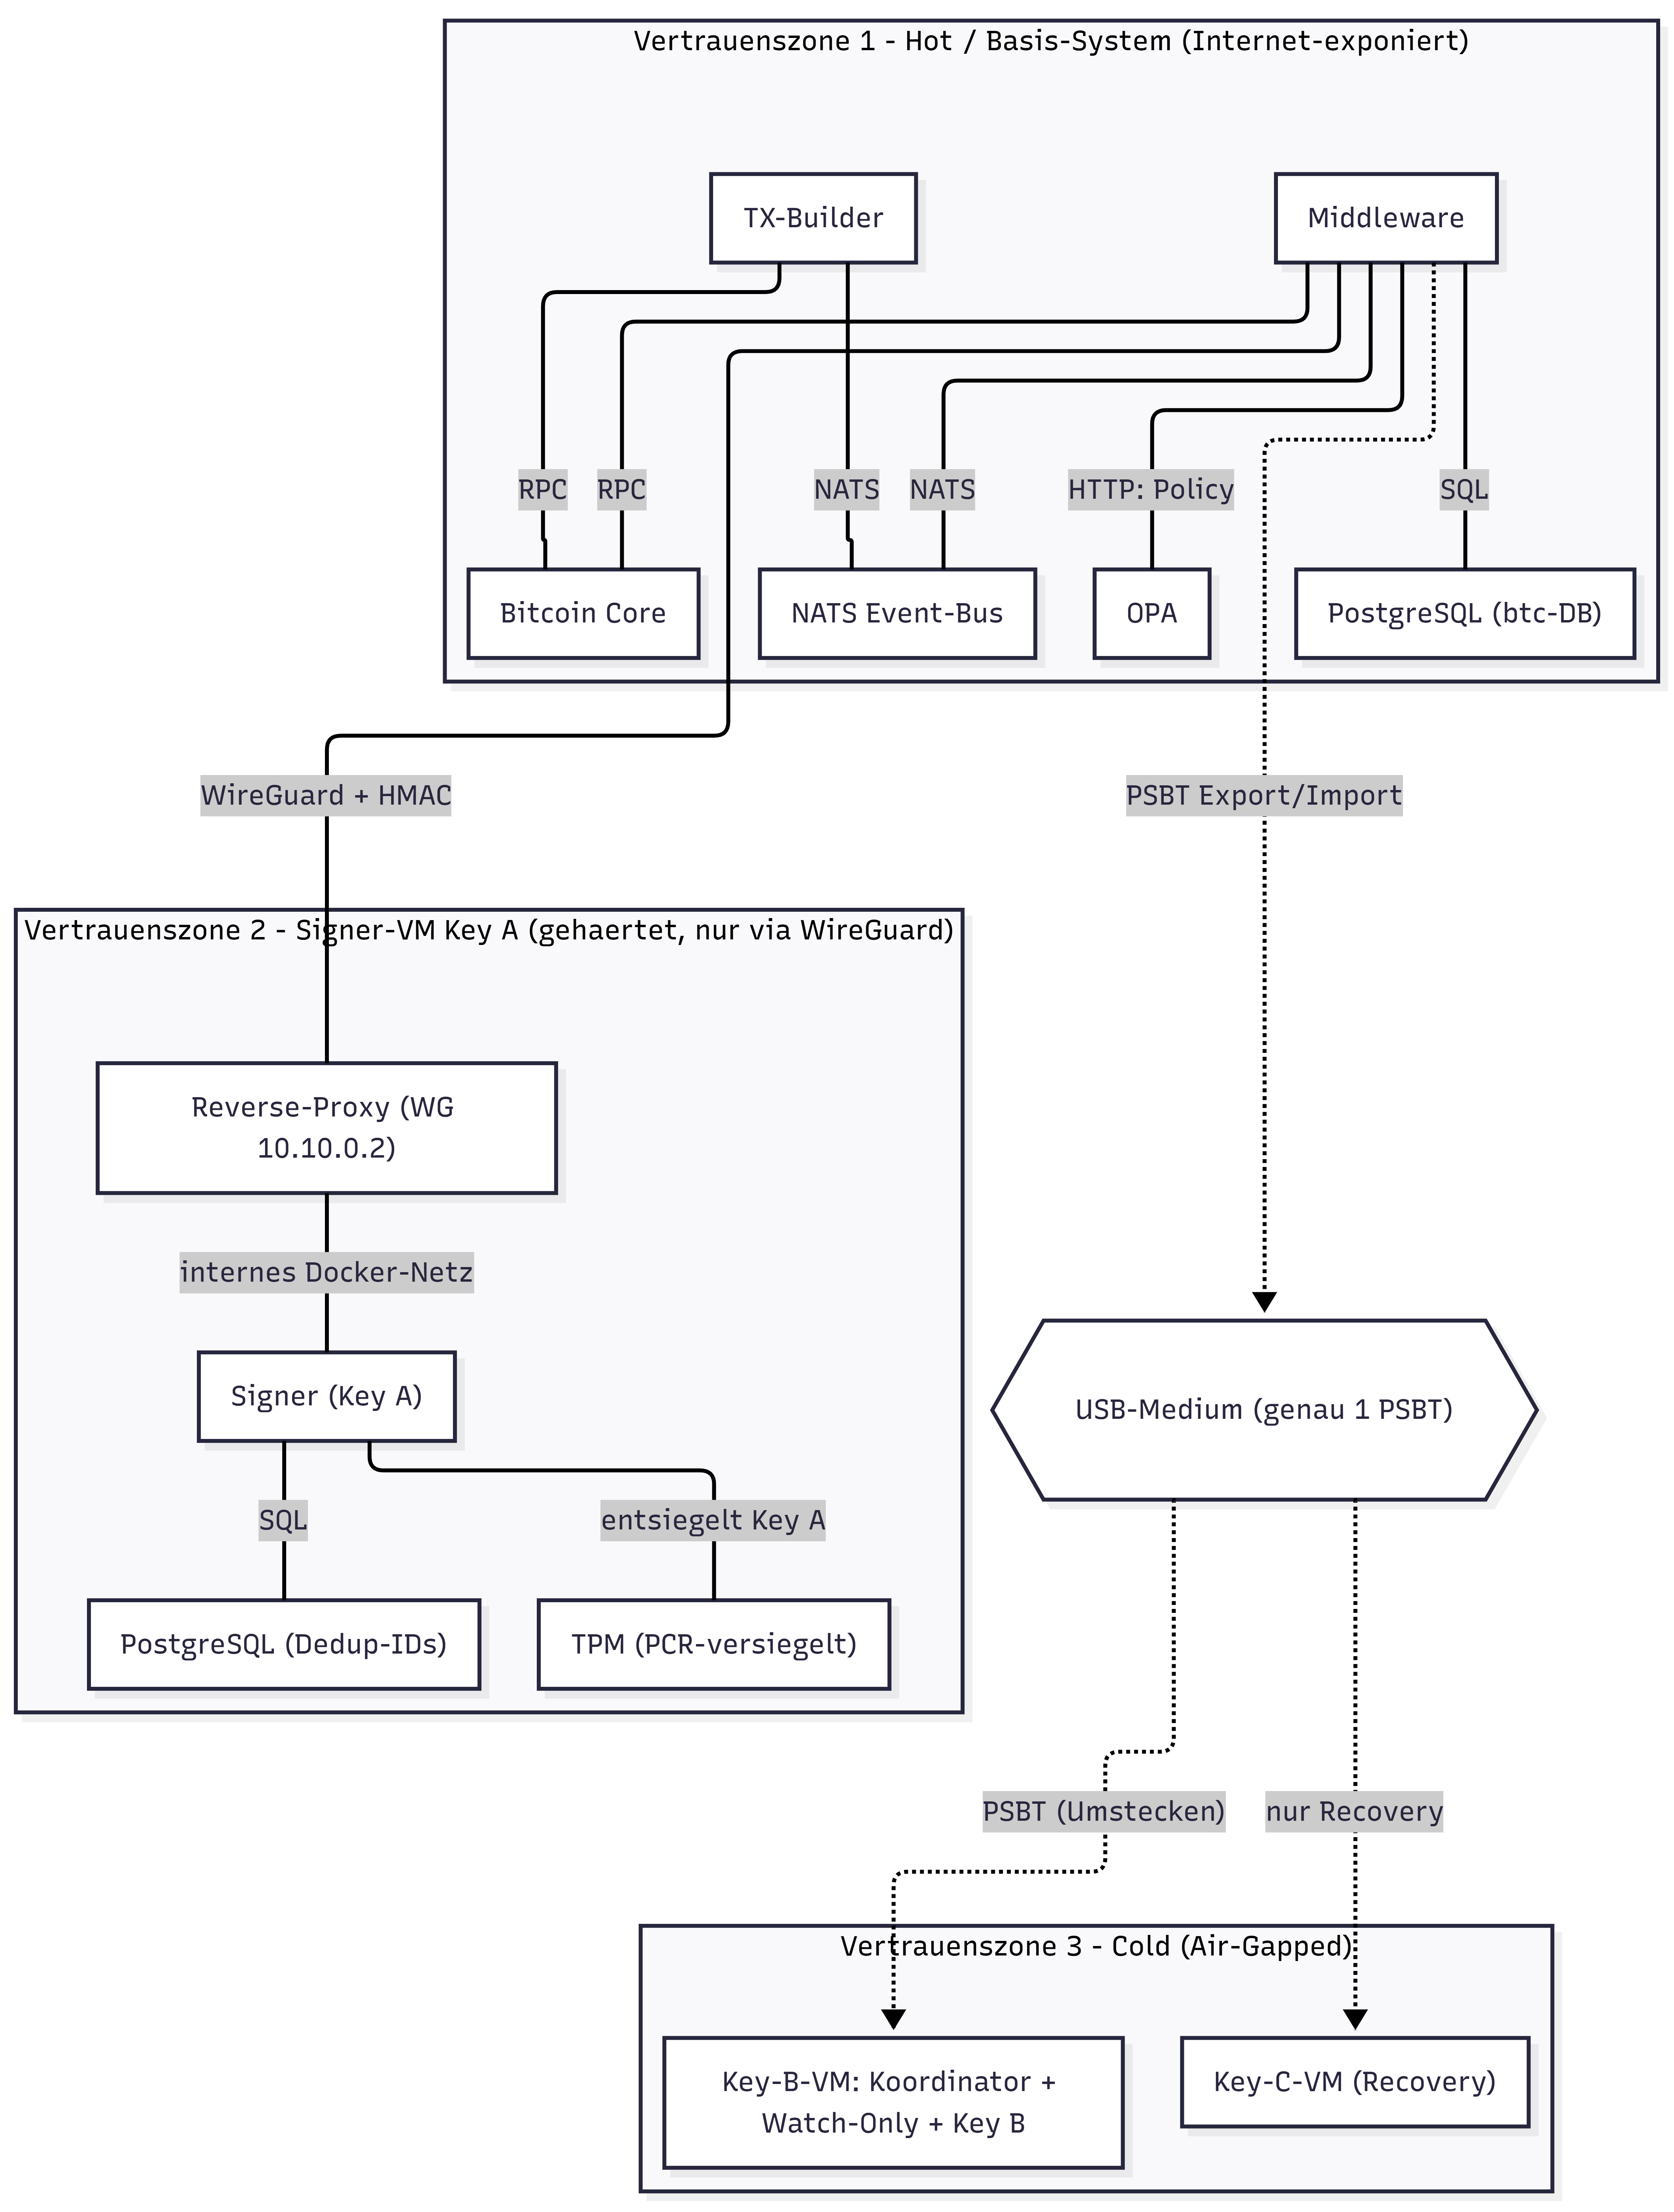
\includegraphics[width=0.8\textwidth]{Doku/Abbildungen/Krypto_Vertrauenszonen.png}
    \caption{Darstellung der PSBT-Vertrauenszonen als Hardwarekomponenten und ihrer gehosteten Services. Quelle: Eigene Darstellung.}
    \label{fig1:krypto_zonen}
\end{figure}

\paragraph{\ac{PSBT}} \mbox{}\\
Als \ac{BIP}~174 wurde das \ac{PSBT}-Format als Standard veröffentlicht und bildet die Grundlage des gesamten Signierprozesses
Ein \ac{BIP} ist ein standardisiertes Dokument des offenen Bitcoin-Entwicklungsprozesses, über das technische Erweiterungen, Formate und Konventionen vorgeschlagen, diskutiert und bei Annahme durch die Community als einheitlicher Standard etabliert werden. \acp{BIP} sind fortlaufend nummeriert und stellen sicher, dass unabhängige Implementierungen (Wallets, Nodes, Bibliotheken) interoperabel bleiben.

\ac{BIP}~174 beschreibt ein einheitliches Austauschformat für eine noch unvollständig signierte \ac{TX}, das alle zur Prüfung und Signierung nötigen Informationen wie Inputs, \acp{UTXO}, Ableitungspfade und Outputs mitführt, ohne private Schlüssel zu enthalten. Dies ermöglicht die Realisierung unseres Ansatzes, eine \ac{TX} über mehrere getrennte Systeme wie Hot-Signer und air-gapped Cold-Signer hinweg schrittweise zu signieren, ohne dass Schlüsselmaterial die jeweilige Zone verlässt. Da alle beteiligten Werkzeuge denselben \ac{BIP}-174-Standard umsetzen, ist die \ac{PSBT} über den gesamten Weg interoperabel verarbeitbar.

Die in \ac{BIP}~174 definierten Rollen wie Creator, Updater, Signer, Combiner,
Input Finalizer und Transaction Extractor beschreiben logische
Verarbeitungsschritte und nicht zwingend getrennte Akteure. Die Spezifikation
sieht ausdrücklich vor, dass eine einzelne Instanz mehrere Rollen gleichzeitig
übernehmen darf \cite{bip174}. Tabelle~\ref{tab:psbt_roles} zeigt die
Zuordnung in der vorliegenden Architektur. Entsprechend ist es zulässig, dass
das Hot-System eine \ac{PSBT} nicht nur erstellt, sondern unmittelbar auch
teilweise signiert, bevor sie an weitere Signierer übergeben wird.

\begin{table}[htbp]
\centering
\footnotesize
\renewcommand{\arraystretch}{1.3}
\begin{tabularx}{\linewidth}{@{} l >{\RaggedRight}X >{\RaggedRight}X @{}}
\toprule
\textbf{\ac{BIP}-174-Rolle} & \textbf{Hot-Pfad} & \textbf{Cold-Pfad} \\
\midrule
Creator / Updater & Bitcoin Core (\texttt{\seqsplit{walletcreatefundedpsbt}}), angestoßen durch den TX-Builder & wie Hot-Pfad \\
\addlinespace
Signer & Key~A (Signer-\ac{VM}, automatisch) & Key~A (1/3, automatisch), Key~B/Key~C (Sparrow, manuell) \\
\addlinespace
Combiner & entfällt (nur eine Signatur) & Sparrow Wallet (Cold-\ac{VM}) \\
\addlinespace
Input Finalizer & Bitcoin Core (\texttt{finalizepsbt}) & Sparrow Wallet \\
\addlinespace
Transaction Extractor & Bitcoin Core (Basis-System) & Sparrow (\path{.txn}-Export), Broadcast über das Basis-System \\
\bottomrule
\end{tabularx}
\caption{Zuordnung der \ac{BIP}-174-Rollen zu den Systemkomponenten}
\label{tab:psbt_roles}
\end{table}

Durch dieses Vorgehen kann die Authentizität der Transaktion bereits vor der Koordination im Cold-Wallet nachgewiesen werden. Dies zeigt, dass sie vom Basis-System verifiziert und nicht im Transit modifiziert wurde. Die nachgelagerten Cold-Signaturen durch Key~B und Key~C ergänzen diese initiale Signatur gemäß dem \ac{PSBT}-Prozess \cite{bip174,sparrow_multisig,learnmeabitcoin_psbt}.

Durch die ausschließliche Nutzung von \acp{PSBT} wird sichergestellt, dass sensitives Schlüsselmaterial das air-gapped System niemals verlässt und keine Signaturschritte außerhalb der expliziten Benutzerinteraktion erfolgen \cite{bip174,psbt_dcentral,nist_zero_trust}.

Zur Gewährleistung einer erhöhten Sicherheit wurde zudem ein Multi-Signatur-Verfahren für das Cold-Wallet etabliert, das sich Schlüssel~A als Single Key mit dem Hot-Wallet teilt (siehe Abbildung~\ref{fig6:cold_signing}).
Dies erhöht die Sicherheit des Cold-Wallets drastisch und bildet einen Kompromiss zur Operationalität des Systems.

\begin{figure}[htbp]
    \centering
    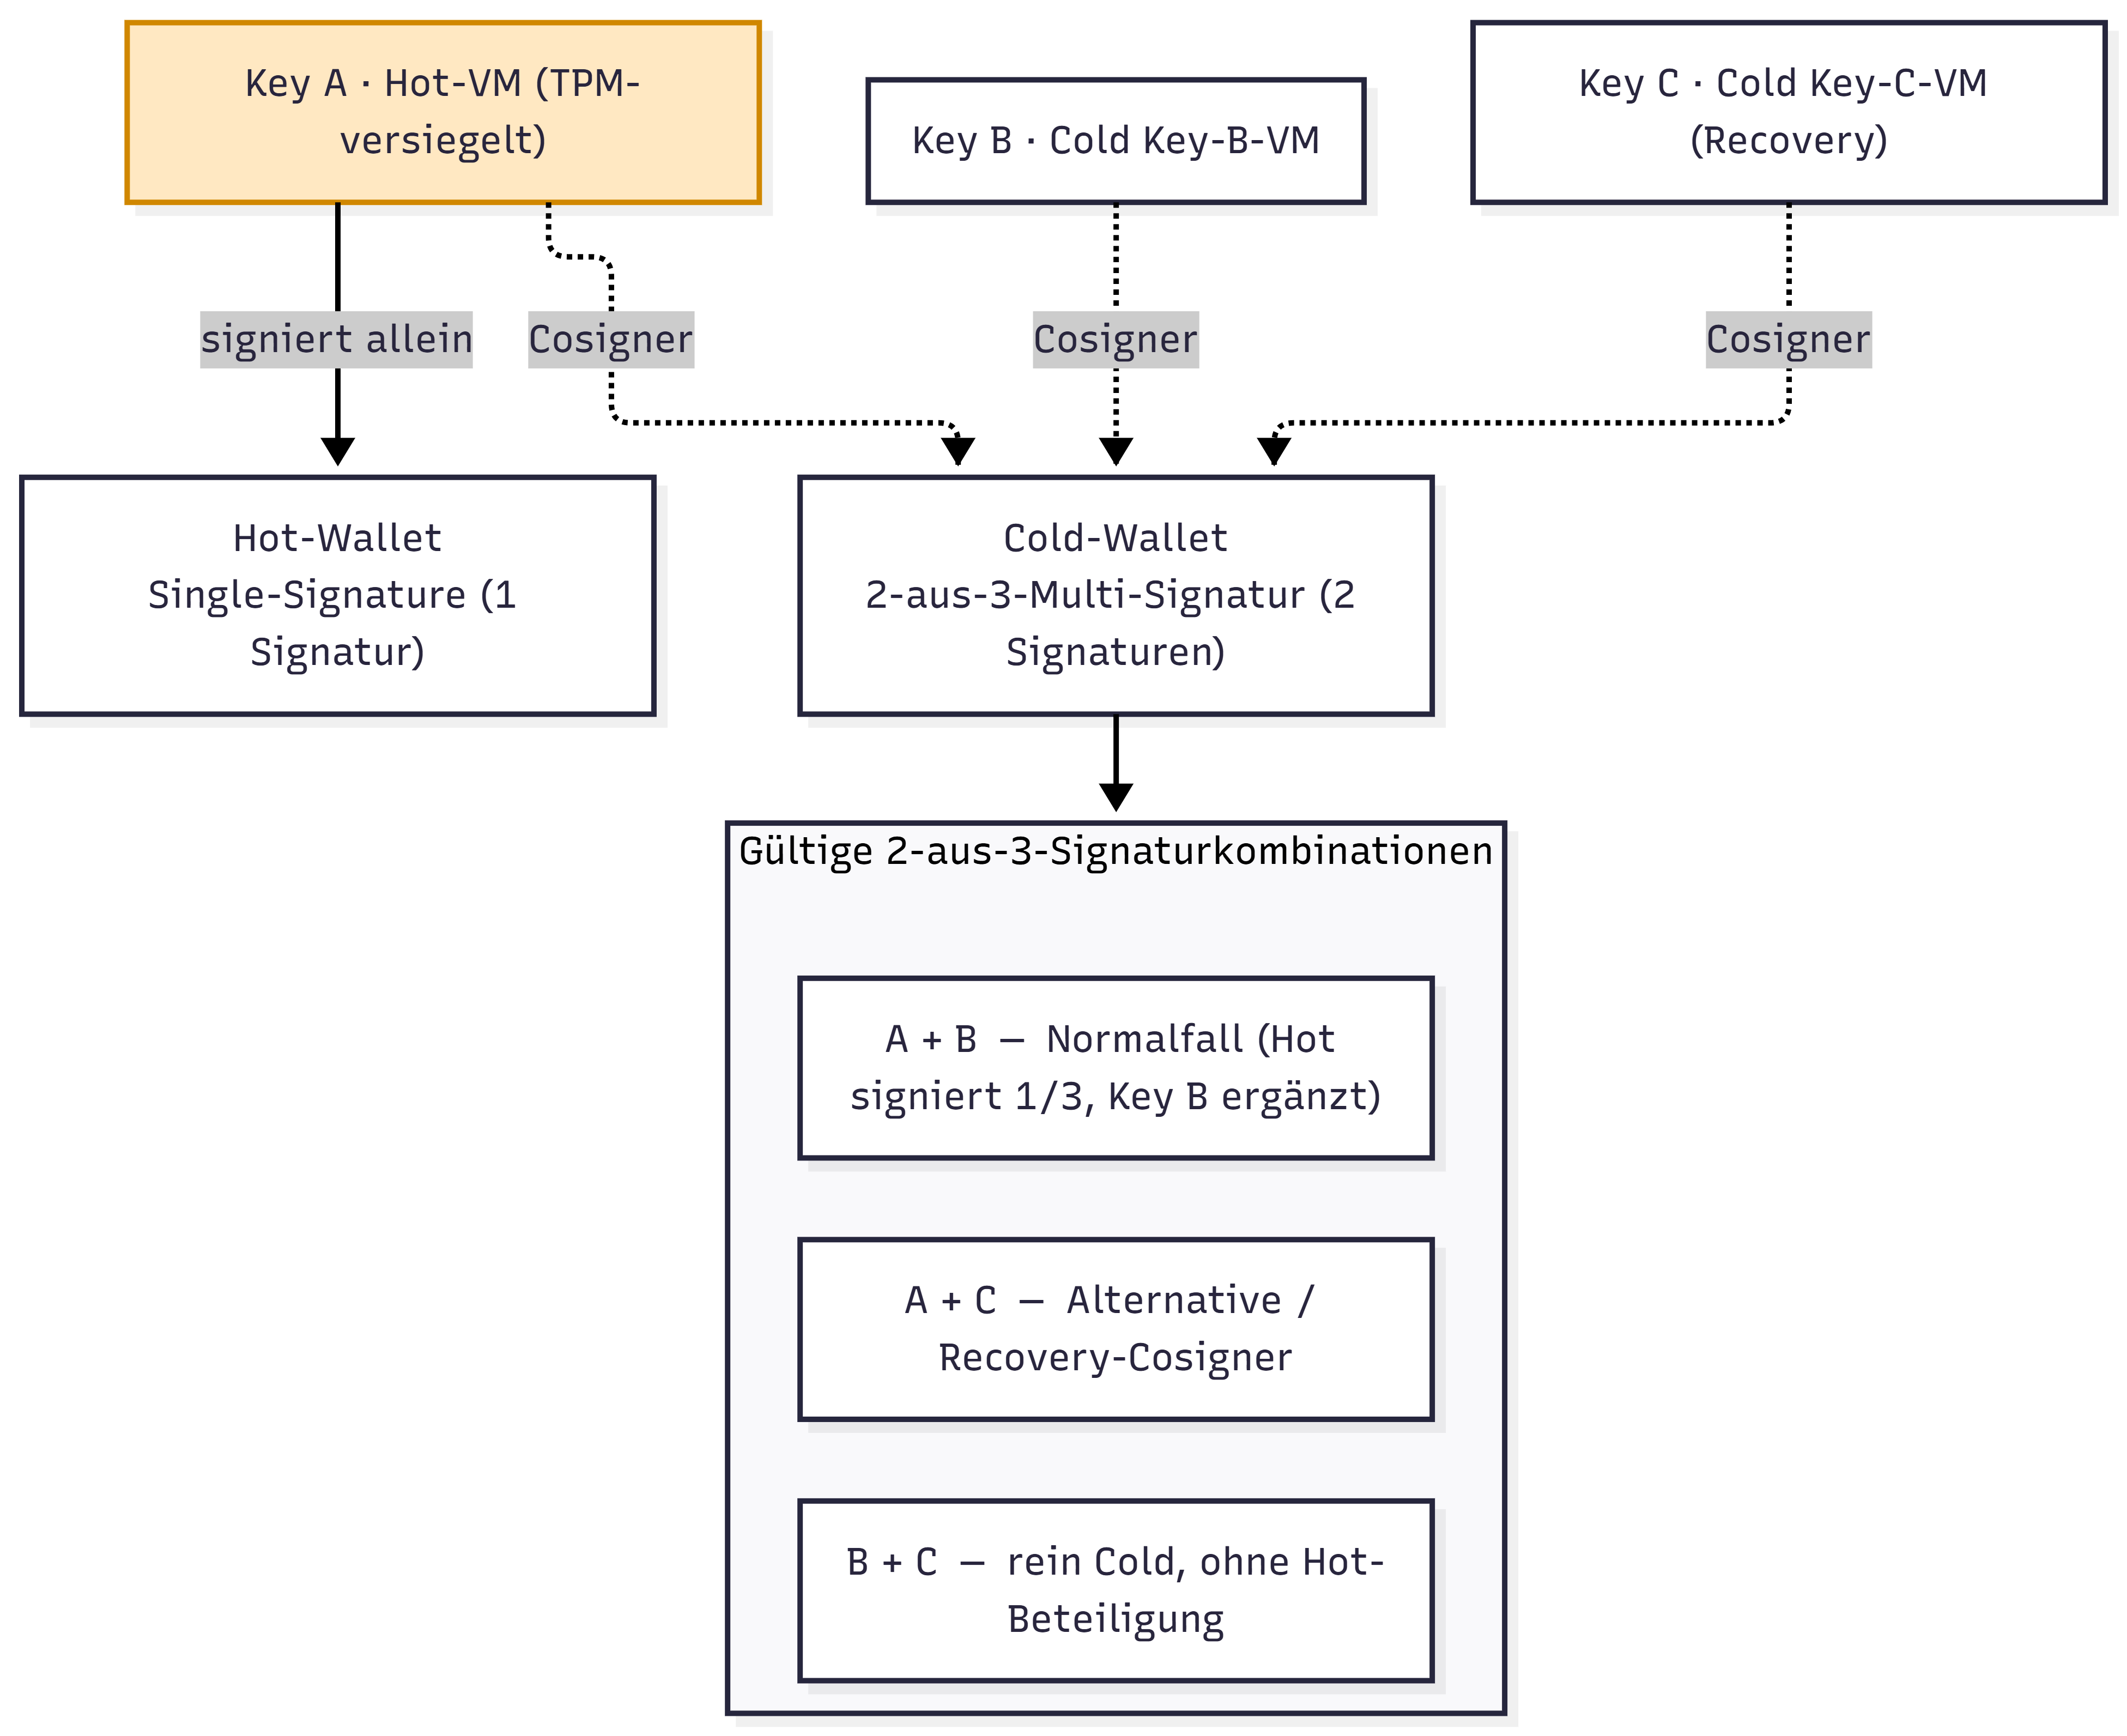
\includegraphics[width=0.8\textwidth]{Doku/Abbildungen/key_Architecture.png}
    \caption{Darstellung der Schlüsselverwendung im Signierprozess. \\Quelle: Eigene Darstellung.}
    \label{fig2:key_architecture}
\end{figure}

Abbildung~\ref{fig1:krypto_zonen} stellt diese Aufteilung als Vertrauenszonen dar.
Jede Hardware-Komponente bestehend aus Hot-Wallet-Basis-System, Signierer-\ac{VM} und den beiden Cold-\acp{VM} bildet eine eigene Zone mit den darauf gehosteten Diensten. Die Abstufung kennzeichnet das Expositionsniveau, von der stark exponierten Online-Zone des Hot-Wallets über die gehärtete, nur per \ac{WG} erreichbare Signierer-Zone bis zur vollständig isolierten, air-gapped Cold-Zone. Zwischen den Zonen werden ausschließlich \acp{PSBT} ausgetauscht, niemals Schlüsselmaterial.

Während das Hot-Wallet für automatisierte Transaktionen genutzt wird, erfolgen Transfers aus dem Cold-Wallet ausschließlich kontrolliert und bewusst nicht vollautomatisiert mit manueller Freigabe \cite{knowingbitcoin_hotcold, Wallets, Hot_VS_Cold-Wallet, psbt_dcentral}.
Da sich Hot- und Cold-Wallet einen Schlüssel teilen, kann der Cold-Wallet-Prozess bis zur Benachrichtigung des Mandanten parallel zum Hot-Wallet teilautomatisiert ablaufen (siehe Abbildung~\ref{fig2:key_architecture}).

\subsubsection{NixOS}

\paragraph{Deklarative Systemhärtung} \mbox{}\\
Die Schlüsselhalter-\acp{VM} werden über NixOS deklarativ gehärtet, um eine Basis Sicherheit gegen Angreifer gewährleisten zu können.
Die exakt getroffenen Maßnahmen können im Anhang in der Tabelle \ref{tab:nixos_hardening} nachvollzogen werden.

Die schlüsselhaltende Hot-\ac{VM} (Key~A) wird analog gehärtet, ist jedoch nicht vollständig air-gapped, sondern ausschließlich über einen einzelnen, per WireGuard authentifizierten \ac{UDP}-Port erreichbar. Sämtlicher übriger Verkehr wird per \texttt{nftables} verworfen.

\paragraph{Warnung bei der NixOS-Installation} \mbox{}\\
Bei der Installation von NixOS werden die folgenden Warnmeldungen ausgegeben:
\begin{itemize}
    \item \enquote{Mount point '/boot' which backs the random seed file is world accessible, which is a security hole! ...}
    \item \enquote{Random seed file '/boot/loader/.\#bootctlrandom-seedc5706ea22f8895b0' is world accessible, which is a security hole! ...}
\end{itemize}

Diese rühren daher, dass die gesetzten Berechtigungen für die vfat-Boot-Partition nicht erkannt werden.
Diese Warnung wurde recherchiert, ist der Community bekannt und wird als fälschlich ausgelöst und damit unbedrohlich eingestuft \cite{nixOS_warnung}.

\paragraph{Dockerhärtung}

Wie bereits in Abschnitt \ref{sec:apphost-container} erwähnt werden gewisse Härtungen für die Docker-Container im Basis-System vorgenommen.
Diese wurden ebenfalls für die Härtung der separaten Signierer~\ac{VM} von Key~A vorgenommen und schließen sich so dem Sicherheitskonzept an.

\subsection{Hot-Wallet}

Da das Hot-Wallet dauerhaft mit dem Internet verbunden ist, stellt es die am stärksten exponierte Komponente der Architektur dar. Entsprechend wird dieses System besonders gehärtet und folgt strikt dem Prinzip der \emph{Segregation of Duties}. Ziel ist es, zu verhindern, dass ein einzelner Dienst \acp{TX} eigenständig aufbauen, autorisieren und signieren kann \cite{nadcab_custodial_arch, nist_sp800_53}.

Aufgrund dessen wurde die Hot-Bitcoin-Architektur in einzelne Microservices unterteilt, wobei jeder Service eigene Sicherheitsanker und Autorisierungen besitzt.
Dadurch wird sichergestellt, dass die Kompromittierung eines einzelnen Services nicht zu einer vollständigen Übernahme des Systems führt.
Die Infrastruktur teilt sich in Microservices für die direkte \ac{TX}-Verarbeitung und unterstützende Komponenten:

\textbf{Microservices zur Transaktionsverarbeitung}
\begin{itemize}
    \item Bitcoin Core (Blockchain-Zustand und Transaktionsvalidierung),
    \item Middleware (Orchestrierung und interne und externe Kommunikation),
    \item \ac{OPA} (Deklarative Policy-Engine, die \acp{TX} anhand von Regeln autorisiert (im Detail siehe \ref{sec:opa})),
    \item TX-Builder (Transaktionskonstruktion),
    \item Signierer .
\end{itemize}
\textbf{Unterstützende Komponenten}
\begin{itemize}
    \item PostgreSQL (Persistenz von Wallet- und Transaktionsdaten),
    \item \ac{NATS} (Event-basierte Kommunikation zwischen Services),
    \item WireGuard (verschlüsselte Kommunikation zwischen Systemen),
    \item ntfy (Push-Benachrichtigungen an den Operator, siehe \ref{sec:apphost-monitoring}),
    \item Loki / Prometheus (Logging und Monitoring).
\end{itemize}

\subsubsection{Unterstützende Komponenten}
Als unterstützende Komponenten wird die Basis-Infrastruktur bezeichnet, die nicht speziell auf \ac{BTC}-\acp{TX} zugeschnitten ist und so auch von den anderen Services des Self-Hosted-Setups verwendet werden kann beziehungsweise wird.

Wie bei den deklarativ gehärteten Schlüsselhalter-\acp{VM} (siehe Tabelle~\ref{tab:nixos_hardening}) kommt auch im Hot-Wallet für Key~A NixOS zum Einsatz, wodurch eine Vielzahl an Sicherheitsvorkehrungen direkt deklarativ im Betriebssystem vorgenommen werden kann.

\paragraph{Bitcoin Core Node} \mbox{}\\
Bitcoin Core wird verwendet, um eine wesentliche Vereinfachung von Bitcoin-Operationen zu erreichen. Betrieben als Full Node ohne aktivierte Wallet-Funktion übernimmt dieser Service sowohl die Validierung von Blöcken und Transaktionen, die Mempool-Verwaltung als auch Gebührenschätzungen, besitzt jedoch keine kryptographischen Schlüssel \cite{bitcoin_core_docs,Sparrow_Wallets_Node_Connect}.
Stattdessen können Wallets direkt auf Bitcoin Core durch Import von internen und externen öffentlichen Deskriptoren registriert werden, ohne dass geheimes Schlüsselmaterial preisgegeben werden muss. Anhand dieser Information kann der Service die Adressen- und \ac{PSBT}-Generierung für die Bitcoin-Wallet übernehmen.

Im produktiven Umfeld würde Bitcoin Core als Node mit dem Mainnet verbunden, um reale \acp{TX} und \acp{UTXO} zu verfolgen. Zur Entwicklung und Validierung der Architektur simuliert die Node zudem ein lokales \enquote{Regtest}-Netzwerk. Dieses bietet volle Kontrolle über die Blockchain und stellt ein isoliertes, privates Testnetz ohne Verbindung zu externen Peers dar. Coins können dementsprechend lokal erzeugt werden und verursachen keine Kosten.
Für die spätere produktive Nutzung durch den Mandanten ist eine Umstellung von Regtest auf das Mainnet sowohl in Bitcoin Core als auch in der angebundenen Sparrow Wallet erforderlich. Die vollständigen Migrationsschritte sind in \ref{sec:mainnet_migration} beschrieben.

Die Nutzung der automatischen Blockchain-Verwaltung ersetzt einen zuvor evaluierten Ansatz auf Basis eines \ac{ZMQ}-Listeners. Dieser würde Ereignisse für ausgewählte Wallets überwachen und könnte eine Referenz der \acp{UTXO} in deren Besitz extrahieren. Diese Lösung würde eine separate persistierende Logik erfordern, sodass gefundene \acp{UTXO} in eine weitere Datenbank geschrieben werden müssten. Eine besondere Herausforderung stellt dabei die Blockchain-Reorganisation dar, bei der bereits verarbeitete Blöcke einer sogenannten Fork verworfen und bei der Reintegration in die Blockchain durch alternative Ketten ersetzt werden können. Eine korrekte Behandlung dieser Problematik hätte eine komplexe und fehleranfällige Logik mit Betrachtung verschiedener Edge Cases erfordert. Daneben gestaltet sich das Berechnen der Gebühren einer \ac{TX} ebenfalls als sehr aufwendig, da diese dynamisch auf Basis von Mempool-Zuständen, Blockhöhe, Chain-Tips und Netzwerk-Auslastung über mehrere Berechnungen stabilisiert werden müssten.

Durch die Nutzung von Bitcoin Core können diese Aspekte vollständig ausgelagert werden.
Insbesondere ermöglicht die Kombination aus Deskriptor-Import und dem \ac{RPC}-Befehl \texttt{{walletcreatefundedpsbt}} eine einfache Erstellung von Transaktionen \cite{bitcoincore_walletcreatefundedpsbt}.

Zudem erlaubt Bitcoin Core, dynamisch generierte Zieladressen einem registrierten Wallet zuzuordnen, ohne auf statische Adressen angewiesen zu sein, was die Problematik aus \ref{sec:dyn_adress} auflöst. Auf diese Weise wird die Nachvollziehbarkeit von \acp{TX} sichergestellt, während gleichzeitig datenschutzrelevante Anforderungen des Mandanten erfüllt werden.
Dies stellt einen relevanten Aspekt zur Umsetzung der vollautomatischen Partner-Kommunikation dar. Ankommende Anfragen müssen vor Ausführung autorisiert werden, wobei verschiedene Möglichkeiten bestehen. Eine lässt sich in einer engen Absprache mit dem Partner durch den Austausch eines gemeinsamen Geheimnisses (siehe \ref{sec:partner_auth}) oder in der Verwendung von statischen Adressen finden.
Eine einfachere und ebenfalls sichere Möglichkeit wird durch das Vertrauen der Partner-Wallets in Form eines Whitelistings dieser dargestellt. Dabei kann Bitcoin Core diese Wallets über den Import des externen Deskriptors als eigene Wallet registrieren und anschließend die Adresszugehörigkeit zu einer bestimmten Wallet mit \path{getaddressinfo} verifizieren und so freigeben.

Ein zusätzlicher privater Electrum-Server wurde aufgrund des erhöhten Betriebsaufwands und des begrenzten Mehrwerts innerhalb des Projektumfangs, wie bereits in \ref{sec:electrum_serv} erwähnt, nicht implementiert.

\paragraph{PostgreSQL} \label{sec:btc_db} \mbox{}\\
Wie bereits beschrieben, wird PostgreSQL als Datenbank verwendet, um verschiedene Daten über System- oder Docker-Neustarts hinaus zu persistieren.
Hierzu wird eine dedizierte Datenbank \texttt{btc} betrieben, die alle Wallet- und \ac{PSBT}-Informationen umfasst.
Gespeichert werden:
\begin{itemize}
    \item Wallet-Metadaten für Hot-, Cold- und whitelisted externe Wallets,
    \item \ac{PSBT}-Daten und Lebenszykluszustände,
    \item Entscheidungsdaten aus der \ac{OPA}-Policy-Auswertung,
    \item archivierte Transaktionen nach erfolgreichem Broadcast.
\end{itemize}

Der Zugriff auf die \texttt{btc}-\ac{DB} wird ausschließlich über den Middleware-Microservice administriert, um eine einzige Source of Truth darstellen zu können. Dementsprechend werden auf diesem Service verschiedene \acp{API} zum Adressieren der Datenbank bereitgestellt.

\label{sec:wallet_import}
Neben den Hot- und Cold-Wallets werden die Namen externer, whitelisted Wallets in der Wallet-\ac{DB} eingetragen. Dafür wurden die Skripte \path{wallet_import.sh} und \path{whiteWallet.sh} eingerichtet, sodass relevante Informationen wie Registrierungs-Name, Schlüssel-Fingerprint und Deskriptoren für die einzelnen Wallets kontrolliert aus dem Dateiverzeichnig (oder einem\ac{USB}-Medium im Falle eines stand-alone Ansatz des Krypto Sub-System) extrahiert werden können.
Die Registrierung selbst erfolgt nicht über einen \ac{HTTP}-Endpunkt, sondern ereignisgesteuert über \ac{NATS}, da sich eine nicht-internet exponierte Schnittstelle als sicherer erweist.
Die Setup-Identität veröffentlicht \texttt{\seqsplit{wallet.import.requested}}, woraufhin die Middleware das Wallet in Bitcoin Core und PostgreSQL einträgt und den Ausgang über \texttt{\seqsplit{wallet.import.done}} bzw.\ \texttt{\seqsplit{wallet.import.failed}} zurückmeldet.

Zusätzlich zu den für den Betrieb notwendigen Daten werden ebenfalls der vollständige Statusverlauf jeder \ac{PSBT} sowie die Entscheidungen des \ac{OPA} samt Begründung und Input gespeichert, und die \ac{PSBT} wird nach dem Broadcast als Artefakt archiviert.
Nach dem Broadcast am Ende des \ac{PSBT}-Prozesses wird die verwendete \ac{PSBT} im Sinne einer Archivierung in der Tabelle \path{btc.psbt_archive} gespeichert. Die Tabelle \path{btc.psbt}, welche die einzelnen Status nach den Microservice-Schritten enthält, soll dementsprechend eher als Runbook zum Nachvollziehen des operationellen Verlaufs der \ac{TX} verstanden werden und kann nach einer gewissen Zeit gelöscht werden.
Der vollständige Lebenszyklus einer \ac{PSBT} mit allen Zustandsübergängen ist in Abbildung~\ref{fig8:psbt_states_visual} grafisch dargestellt, während die exakten Beschreibungen der einzelnen Zustände im Anhang in Tabelle~\ref{tab:psbt_states} nachgelesen werden können.

\begin{figure}[htbp]
    \centering
    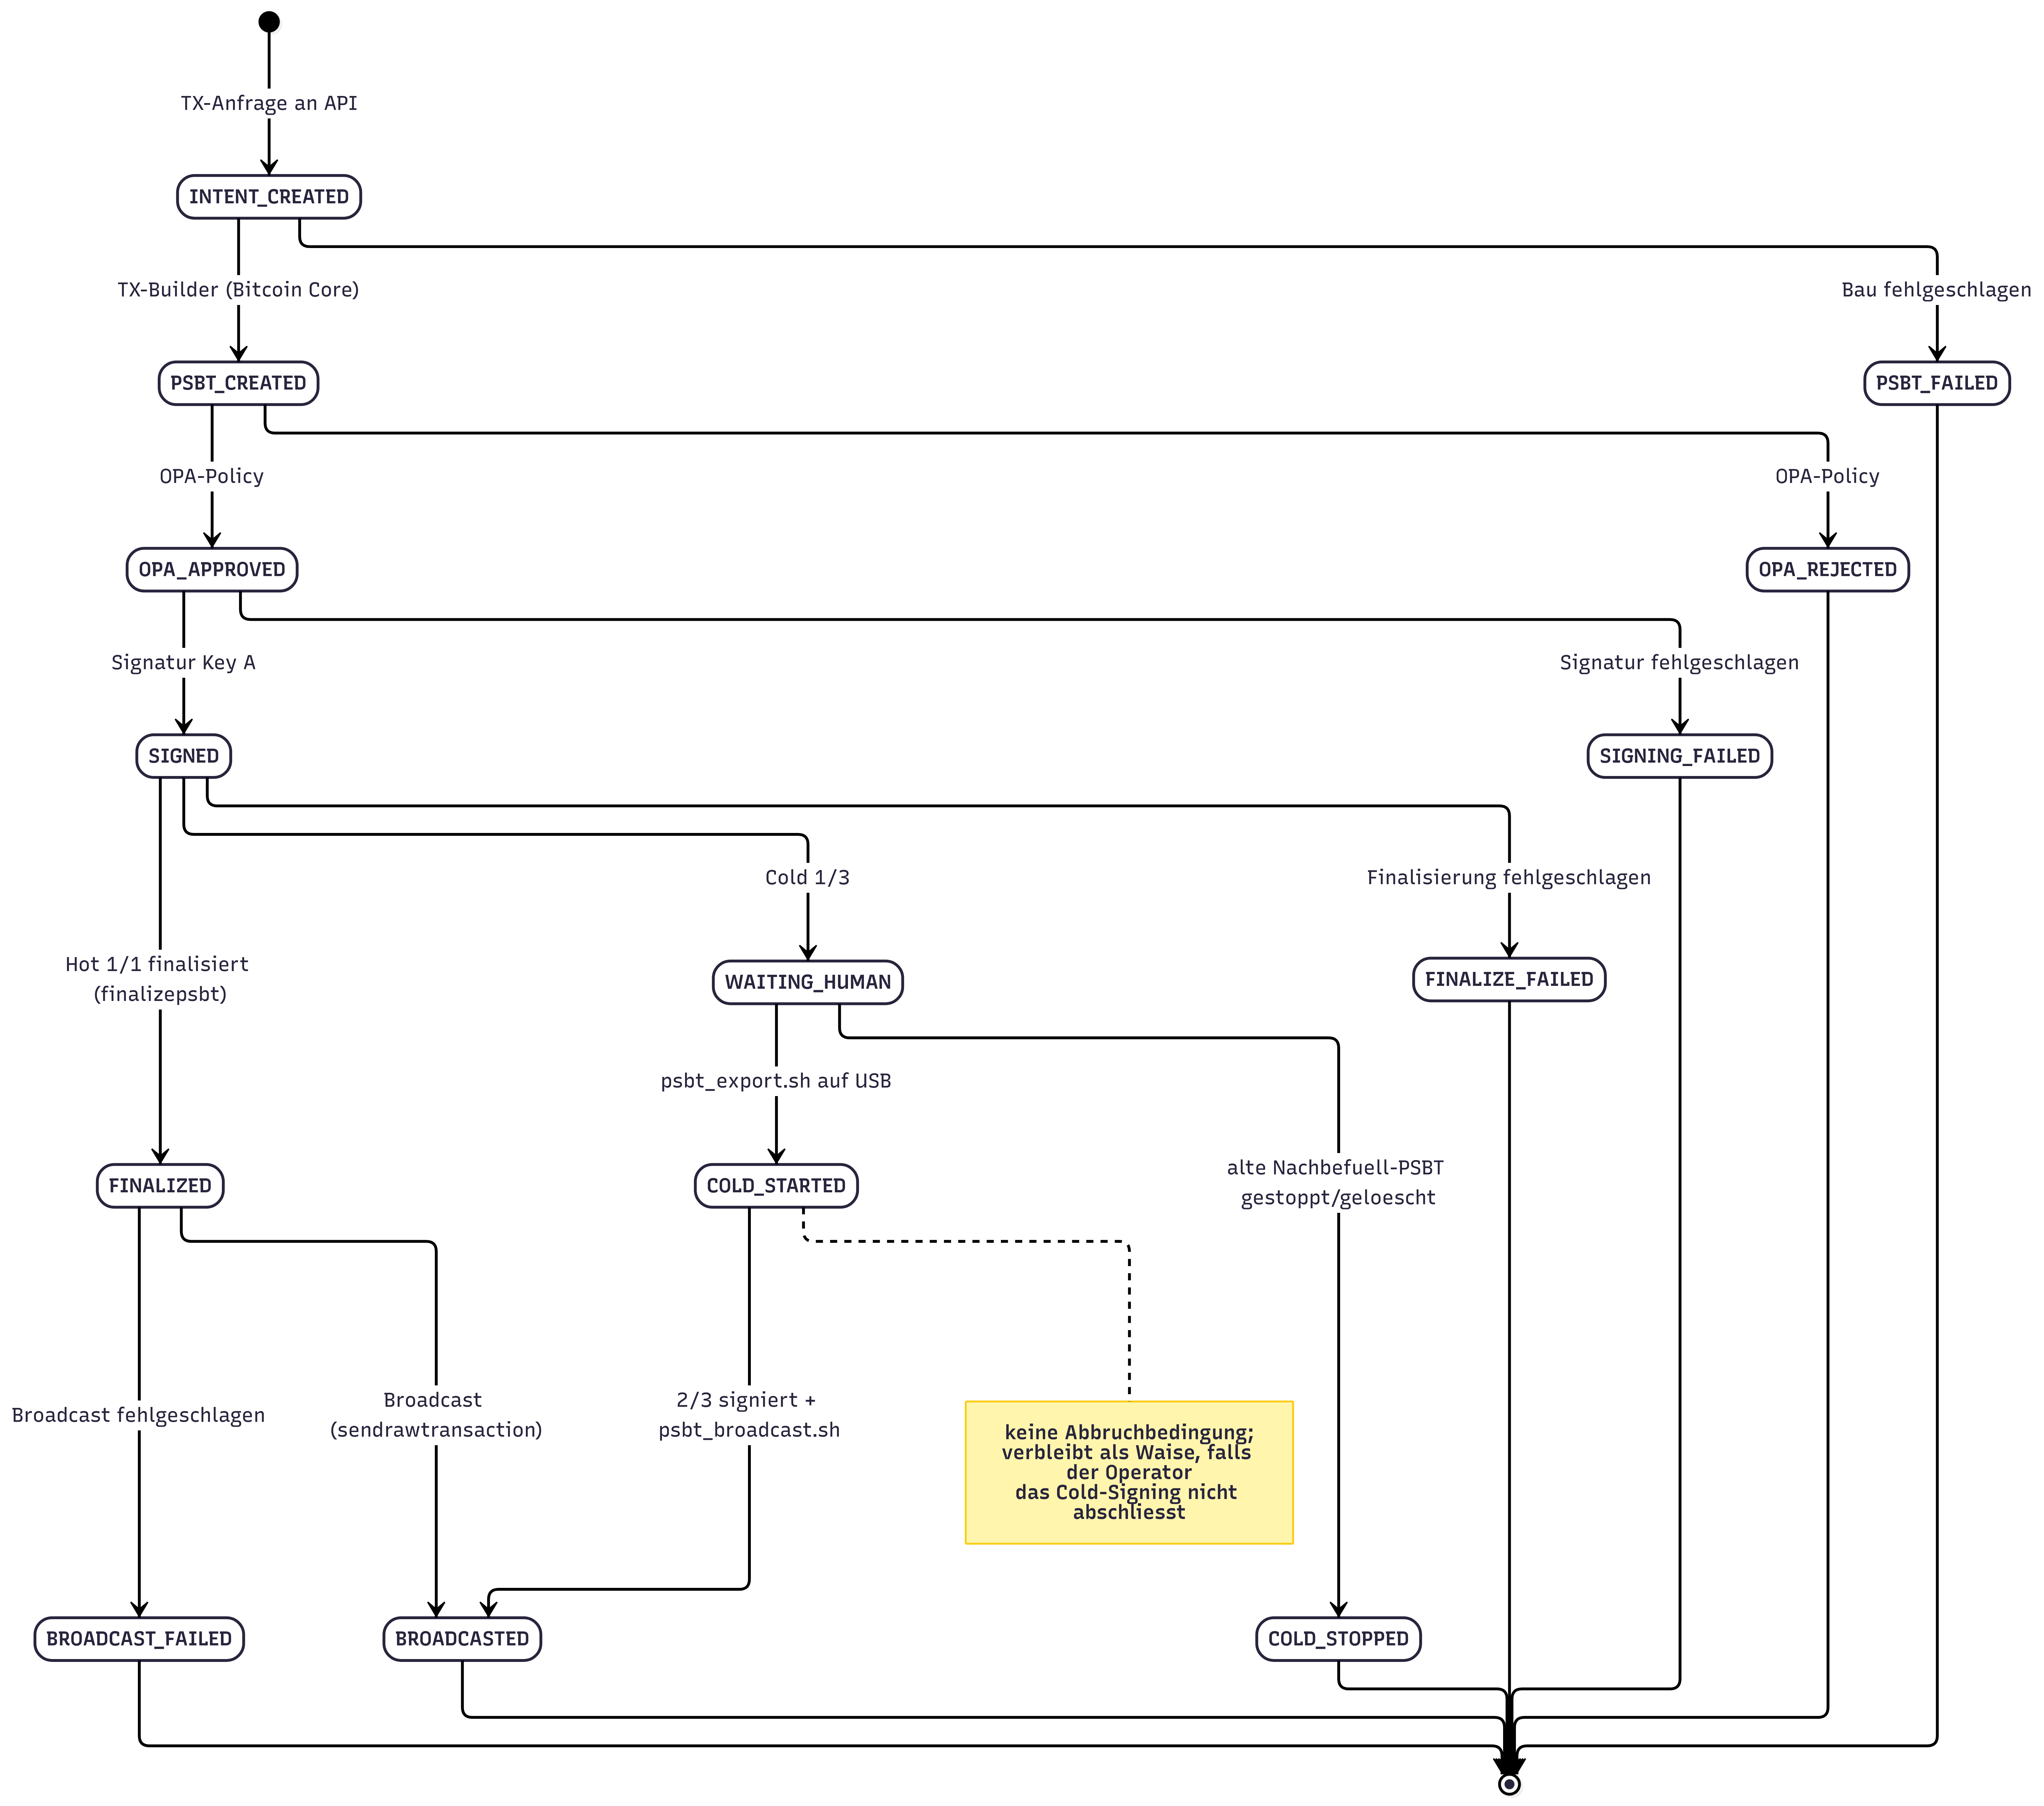
\includegraphics[width=1.0\textwidth]{Doku/Abbildungen/PSBT_state.png}
    \caption{PSBT-Lebenszyklus und Statusübergänge. Quelle: Eigene Darstellung.}
    \label{fig8:psbt_states_visual}
\end{figure}

\paragraph{\ac{NATS}} \mbox{}\\
Die Event-basierte Kommunikation zwischen den Microservices wird über den Messaging-Service \ac{NATS} realisiert. \ac{NATS} implementiert ein Publish-Subscribe-Modell, bei dem Nachrichten auf sogenannten Subjects veröffentlicht und von mehreren Empfängern empfangen werden können. Durch eine besonders geringe Latenz eignet sich \ac{NATS} gut für Echtzeitkommunikation, wie sie für unseren Anwendungsfall beispielsweise zur Wahrung der Aktualität von Gebühren einer \ac{TX} benötigt wird.

Um die Eskalationsmöglichkeit bei Kompromittierung eines einzelnen Dienstes weiter zu verringern, wurde sich für die Implementation eines Autorisierungs-Mechanismus entschieden.
Andernfalls könnte ein Angreifer aus einem Docker-Container heraus \ac{NATS}-Nachrichten fälschen und damit andere Services in Form eines Lateral Movement korrumpieren.
Als zusätzliche Härtung erhält jeder Microservice eine eigene, dedizierte \ac{NATS}-Identität mit einer explizit definierten Publish- und Subscribe-Berechtigung (siehe Tabelle~\ref{tab:nats_permissions}), die exakt der im Applikationscode bereits bestehenden Verantwortungstrennung entspricht. Die zulässigen Subjects je Dienst ergeben sich unmittelbar aus dem Nachrichtenfluss des Systems.
\begin{table}[htbp]
\centering
\begin{tabular}{|l|p{6.0cm}|p{6.0cm}|}
\hline
\textbf{Service} & \textbf{Publish} & \textbf{Subscribe} \\
\hline
Middleware & \texttt{intent.created}, \texttt{psbt.build.requested}, \texttt{psbt.created}, \texttt{wallet.import.done}, \texttt{wallet.import.failed} & \texttt{intent.created}, \texttt{psbt.created}, \texttt{psbt.failed}, \texttt{refill.export.done}, \texttt{refill.broadcast.requested}, \texttt{psbt.submit.requested}, \texttt{wallet.import.requested} \\
\hline
TX-Builder & \texttt{psbt.created}, \texttt{psbt.failed} & \texttt{psbt.build.requested} \\
\hline
Operator & \texttt{refill.export.done}, \texttt{refill.broadcast.requested}, \texttt{psbt.submit.requested} &  \\
\hline
Setup & \texttt{wallet.import.requested} & \texttt{wallet.import.done}, \texttt{wallet.import.failed} \\
\hline
\end{tabular}
\caption{Subject-Berechtigungen je Microservice}
\label{tab:nats_permissions}
\end{table}

Entscheidend ist dabei nicht die vollständige Symmetrie der Matrix, sondern die gezielte Einschränkung des nachgelagerten Dienstes: Der TX-Builder erhält ausschließlich das Recht, Ergebnis-Events zu veröffentlichen und Bau-Aufträge zu empfangen. Das Veröffentlichen von \texttt{\seqsplit{intent.created}} ist ihm verwehrt. Eine Kompromittierung des TX-Builders bleibt dadurch auf das Einschleusen fehlerhafter \acp{PSBT} beschränkt. Dieser Angriffsvektor, der durch die nachgelagerte \ac{OPA}-Autorisierung und die Whitelist-Prüfung der Zieladresse ohnehin abgefangen wird, kann den Prozess nicht zusätzlich an seinem Ursprung manipulieren.

Die Zugangsdaten der einzelnen \ac{NATS}-Identitäten werden, analog zu den bereits beschriebenen Datenbank-Zugangsdaten, nicht statisch in der versionierten Konfiguration hinterlegt. Stattdessen werden sie bei der Initialisierung der Key~A \ac{VM} erzeugt und in einer restriktiv berechtigten Laufzeitdatei außerhalb der Versionskontrolle gehalten, auf die ausschließlich die beteiligten lokalen Prozesse Zugriff besitzen. In Verbindung mit der Netzwerkisolation, durch welche der \ac{NATS}-Server keinen nach außen gerichteten Port besitzt, werden so sowohl ein direkter externer Zugriff als auch eine dienstübergreifende Rechteausweitung über den Event-Bus ausgeschlossen \cite{NATS_Auth}.

Eine weitergehende Ausbaustufe besteht in der Umstellung von der statischen, passwortbasierten Autorisierung auf ein dezentrales, auf NKeys und JSON Web Token basierendes Account-Modell. Dieses würde eine kryptografisch verankerte Identität je Dienst sowie eine signierte Rechtevergabe ermöglichen und die Verwaltung der Berechtigungen von der Server-Konfiguration entkoppeln. Aufgrund des erhöhten Verwaltungsaufwands und des für den aktuellen Projektumfang bereits hinreichenden Schutzniveaus der statischen Variante wurde diese Ausbaustufe als optionale Erweiterung eingestuft.

In Kombination mit \ac{NATS} wird \ac{HTTP} als \ac{API} für gezielte GET-Abfragen zwischen Containern verwendet, wenn Informationen für den weiteren Prozessverlauf abgefragt statt Ereignisse ausgelöst werden. Die Transportwege sind dabei klar getrennt, sodass über \ac{HTTP} ausschließlich die externen Eingänge (\texttt{BIP21}/\texttt{PSBT}, siehe Tabelle~\ref{tab:tx_rails}), der Signier-Aufruf an die Key~A \ac{VM} (\texttt{POST /sign}) sowie die Health- und Metrics-Endpunkte laufen. Alle betreiberausgelösten internen Abläufe wie die manuelle \ac{PSBT}-Einreichung, der Abschluss des Wechselmedium-Exports und der Broadcast der signierten Cold-\ac{PSBT} werden hingegen über \ac{NATS} unter der Operator-Identität ausgelöst (\texttt{\seqsplit{psbt.submit.requested}}, \texttt{\seqsplit{refill.export.done}}, \texttt{\seqsplit{refill.broadcast.requested}}) und besitzen bewusst keinen nach außen gerichteten \ac{HTTP}-Endpunkt. Eine frühere \ac{HTTP}-Variante dieser Operator-Aufrufe wurde zugunsten dieser einheitlichen, über die \ac{NATS}-Berechtigungen abgesicherten Ereignissteuerung entfernt.

\paragraph{\ac{WG}} \mbox{}\\
\ac{WG} beziehungsweise sein gebildeter Tunnel stellt den einzigen Kommunikationspfad zwischen dem Hot-Basis-System (Middleware) und der Signierer-\ac{VM} (Key~A) dar, wodurch die Signierer-\ac{VM} von keinem anderen System erreichbar ist. Übertragen werden ausschließlich die zu signierenden \acp{PSBT} vom Basis-System zur Signierer-\ac{VM} und zurückgegeben werden die signierten \acp{PSBT}. Das geheime Schlüsselmaterial wird nicht ausgetauscht und verlässt zu keinem Zeitpunkt die \ac{VM} von Key~A (siehe \ref{sec:in_transit_vault}).

Der Tunnel bildet damit eine eigenständige Authentifizierungs- und Verschlüsselungsschicht für die \ac{API}-Verbindung und erfüllt die Aufgaben:
\begin{itemize}
    \item Absicherung der Datenübertragung durch Transportverschlüsselung zwischen den beiden Peers,
    \item Einschränkung der Kommunikationspfade auf definierte, kryptographisch identifizierte Peers,
    \item Reduktion der Angriffsfläche durch Blockierung aller nicht notwendigen Ports.
\end{itemize}

Die Verbindung basiert auf einem schlanken \ac{UDP}-Protokoll und nutzt moderne kryptographische Verfahren zur Authentifizierung und Schlüsselvereinbarung.
Diese Konfiguration erfolgt zum einen deklarativ per oneShot über NixOS und zum anderen als automatisiertes Skript, sodass reproduzierbare und gehärtete Netzwerkkonfigurationen ermöglicht werden.
Für das besonders kritische Schlüsselmaterial auf NixOS können so alle Ports außer dem \ac{UDP}-Port für den WireGuard-Handshake und -Datenpakete blockiert werden \cite{wireguard}.

Die Peer-Einrichtung und der HMAC-Austausch erfolgen über beiliegende Setup-Skripte auf beiden Systemen. Deren Verwendung ist in den READMEs der Repositories dokumentiert \cite{NixOsHot_github, Krypto_Basis_github}. Eine Kurzübersicht aller Skripte bietet Tabelle~\ref{tab:skripte} im Anhang.

Ergänzend zur Tunnel-Verschlüsselung wird jede Anfrage an die Signierer-\ac{VM} mit einem \ac{HMAC} über ein gemeinsames Geheimnis signiert. Dieses \ac{HMAC}-Geheimnis wird einmalig über das Wechselmedium ausgetauscht und bildet eine zweite, von WireGuard unabhängige Schicht, die Authentizität und Integrität jedes einzelnen Signierauftrags nachweist (siehe \ref{sec:HMAC}). Es genügt somit nicht, in den Tunnel zu gelangen, denn ohne Kenntnis des \ac{HMAC}-Geheimnisses wird eine Anfrage abgewiesen.


\paragraph{Monitoring} \mbox{}\\
Ein zentrales Monitoring überwacht den vollständigen \ac{TX}-Lifecycle sowie den Zustand des Hot-Wallets.
Erfasst werden unter anderem Wallet-Balance, ausstehende Transaktionen und definierte Überweisungsentscheidungen, persistiert in den PostgreSQL-Tabellen des Systems (siehe \ref{sec:btc_db}).
Eine eigene Monitoring-Infrastruktur betreibt der Krypto-Stack dabei bewusst nicht, sondern schließt sich an den im Apphost-Kapitel beschriebenen Stack aus
Prometheus, Loki und Grafana an (siehe \ref{sec:apphost-monitoring}). Dazu exponiert die Middleware unter \path{/metrics} Lifecycle-Metriken im
Prometheus-Format und stellt unter anderem Zähler für eingehende Intents, \ac{PSBT}-Bau, \ac{OPA}-Entscheidungen, Whitelist- und Limit-Ablehnungen sowie
Signier- und Broadcast-Ergebnisse bereit, die der zentrale Prometheus pull-basiert abholt.
Sämtliche Services schreiben zudem strukturierte JSON-Logs, die von Promtail eingesammelt und in Loki abgelegt werden, sodass Metriken und Logs in
Grafana gemeinsam auswertbar sind. Auffälligkeiten oder Grenzwertverletzungen werden automatisiert gemeldet und ermöglichen eine schnelle operationelle
Reaktion. Für deren Zustellung wird ebenfalls der dort beschriebene, selbst gehostete ntfy-Dienst mitgenutzt.

Ebenfalls wird Sparrow als Watch-Only-\ac{GUI} integriert, um einem menschlichen Operator das Verfolgen der \acp{TX} und Wertgegenstände zu ermöglichen \cite{Sparrow_Wallets_Features}.


\subsubsection{Microservices zur Transaktionsverarbeitung}

\paragraph{Middleware} \mbox{}\\
Die Kommunikation und Koordination der einzelnen Services erfolgt über eine dedizierte Orchestrierungskomponente, welche den gesamten Transaktionsprozess steuert (siehe Abbildung~\ref{fig1:krypto_zonen}, woebi der Ablauf selbst wird in \ref{sec:hot_flow} beschrieben).
Die Middleware stellt neben dem \ac{NATS}-Event-Manager sowohl interne als auch externe Schnittstellen bereit und übernimmt die direkte Kommunikation über \ac{HTTP} und \ac{NATS}. Ihre Aufgaben sind:
\begin{itemize}
    \item Entgegennahme externer und operatorseitiger Eingänge (Übersicht in Tabelle~\ref{tab:tx_rails}),
    \item interne Schreib- und Lesebefehle für die PostgreSQL-\ac{DB},
    \item Weiterleitung von Events über \ac{NATS} an interne Services,
    \item Import und Verteilung von Wallet-Metadaten,
    \item Kommunikation mit der Signer-\ac{VM} über eine abgesicherte \ac{HTTP}-Schnittstelle.
\end{itemize}

Der Empfang einer externen Anfrage startet den vom Mandanten geforderten automatisierten Transaktionsprozess (siehe \ref{sec:hot_flow}). Der Umfang der implementierten Schnittstellen aus der realen Welt beschränkt sich bewusst auf \ac{BIP}21-\acp{URI} sowie \ac{PSBT}-basierte Anfragen. Erweiterungen wie das Lightning Network oder Smart-Contract-basierte Ansätze wurden als Erweiterungen des Bitcoin-Netzwerks und damit als außerhalb des aktuellen Anspruchs des Mandanten betrachtet. Weitere Schnittstellen zur Kommunikation mit externen Partnern liegen im Ermessen des Mandanten und können durch Transformation der Eingabe und Auslösen des korrespondierenden \ac{NATS}-Events implementiert werden.
Für die integrierten Schnittstellen gilt:
\begin{itemize}
    \item \ac{BIP}21-Anfragen durchlaufen den vollständigen Prozess inklusive \ac{PSBT}-Erstellung,
    \item bereits vorliegende \acp{PSBT} werden direkt im nächsten Schritt durch \ac{OPA} evaluiert.
\end{itemize}

Nach dem Auslösen der \ac{BIP}21-Schnittstelle wird geprüft, ob der Partner eine Identifikation über das Code-Wort \texttt{id} mitgeliefert hat. Anschließend wird in der Datenbank abgefragt, ob ein Intent mit dieser \ac{ID} bereits bekannt ist. Dadurch werden Duplikate, beispielsweise als Resultat einer Race Condition, vermieden und die Stabilität des Systems durch eine eindeutige Identifikation der Partner-Anfragen erhöht. Zu beachten ist ebenfalls, dass mit den unterschiedlichen Partnern eine hinreichende Nomenklatur ausgehandelt werden muss, sodass diese weder eigene noch fremde \ac{ID}-Räume wiederverwenden. Sollte keine \ac{ID} festgelegt sein, wird eine neue, in der \ac{DB} noch unvergebene UUIDv4 ausgewählt und als \ac{API}-Antwort zurückgegeben \cite{bip21}.

Jegliche Statusveränderung im Prozess wird in der \ac{PSBT}-\ac{DB} geloggt und kann darüber nachvollzogen werden. Zudem wird die Entscheidung des \ac{OPA} samt Begründung und Eingabe separat in \path{btc.opa_decision} persistiert.

Insgesamt lassen sich die Auslöser einer Transaktion in vier Rails einteilen: die beiden externen \ac{HTTP}-Eingänge \texttt{BIP21} und \texttt{PSBT}, den über \ac{NATS} ausgelösten manuellen Operator-Pfad \texttt{manual} sowie die intern durch \ac{OPA} erzeugten Austausch-Transaktionen \texttt{OPA\_hot} und \texttt{OPA\_cold} (siehe Tabelle~\ref{tab:tx_rails}).

\begin{table}[htbp]
\centering
\footnotesize
\setlength{\tabcolsep}{4pt}
\renewcommand{\arraystretch}{1.2}
\begin{tabularx}{\linewidth}{@{} l >{\RaggedRight}X c c c @{}}
\toprule
\textbf{Rail} & \textbf{Auslöser} & \textbf{Whitelist} & \textbf{\ac{OPA} Betrag/Fee} & \textbf{Daily-Cap} \\
\midrule
\texttt{BIP21}  & \ac{HTTP} \texttt{\seqsplit{/api/v1/request/bip21}} & ext & ja & ja \\
\texttt{psbt}   & \ac{HTTP} \texttt{\seqsplit{/api/v1/request/psbt}}  & ext & ja & ja \\
\texttt{manual} & \ac{NATS} \texttt{\seqsplit{psbt.submit.requested}} (Operator, fertige \ac{PSBT}) & Bypass & übersprungen & ja \\
\texttt{OPA\_hot}/\texttt{OPA\_cold} & interne Tauschlogik & interne Wallets & übersprungen & -- \\
\bottomrule
\end{tabularx}
\caption{Transaktions-Rails und ihre Prüfstufen}
\label{tab:tx_rails}
\end{table}

\paragraph{Operator-/Manual-Pfad} \mbox{}\\
Der in Tabelle~\ref{tab:tx_rails} aufgeführte manuelle Operator-Pfad erlaubt es dem Operator, eine eigene, bereits fertig erstellte \ac{PSBT} einzureichen. Es wird empfohlen, diese in einer weiteren Sparrow-Instanz mit dem Hot-Schlüssel als Watch-Only-Wallet zu bauen. Eingereicht wird sie über das Skript \path{scripts/ops/psbt_submit.sh}. Ausgelöst wird der Pfad nicht über \ac{HTTP}, sondern über das \ac{NATS}-Subject \texttt{\seqsplit{psbt.submit.requested}} unter der dedizierten Operator-Identität. Die eingereichte \ac{PSBT} wird unmittelbar als \texttt{\seqsplit{psbt.created}} in den Prüf- und Signierfluss übergeben und überspringt dabei den TX-Builder, da kein Aufbau der \ac{TX} mehr erforderlich ist.

\paragraph{TX-Builder} \mbox{}\\
Nach vollständiger Intent-Entgegennahme an der \ac{HTTP}-Schnittstelle wird dieser zum Bauen der \ac{PSBT} an den TX-Builder-Service weitergeleitet.
Wie bereits erwähnt, war ein vorheriger Ansatz, die \ac{PSBT} direkt im Code selbst zu konstruieren. Dies wurde durch das Extrahieren von \ac{UTXO}-Informationen über \ac{API}-Calls auf die \ac{DB} und über mehrere Stabilisierungs-Durchläufe für die Gebühren ermöglicht.

Dies wurde direkt ersetzt durch die Methode \path{walletcreatefundedpsbt} \cite{bitcoincore_walletcreatefundedpsbt}, welche automatisiert
\begin{itemize}
    \item die Auswahl geeigneter \acp{UTXO},
    \item die Erstellung von Change-Adressen,
    \item die automatische Gebührenschätzung,
    \item die Validierung der verfügbaren Mittel
\end{itemize}
übernimmt.

Für die Standard-Hot-Wallet-\ac{PSBT}-Erstellung überlässt das System die Gebührenwahl bewusst Bitcoin Core. 
Statt einer statischen Fee-Rate wird über
\texttt{conf\_target} eine Bestätigung innerhalb von circa sechs Blöcken ($\approx$ 1~Stunde) im sparsamen \texttt{economical}-Modus angestrebt und die
resultierende Gebühr wird anschließend durch \ac{OPA} validiert (siehe \ref{sec:opa}). 
Watch-Only-\acp{UTXO} und \ac{BIP}32-Ableitungspfade werden in die \ac{PSBT} aufgenommen, da die Signatur erst auf der Key~A \ac{VM} erfolgt.
Replace-by-Fee \cite{bip125} bleibt für reguläre Zahlungen deaktiviert und wird ausschließlich für interne Umschichtungen gesetzt, deren zügige Bestätigung systemkritisch ist. 
Sämtliche Vorgaben können vom Mandanten in der Applikationslogik angepasst werden.

Für Nachbefüllungs- und Sicherungs-Intents bestimmt der \ac{OPA} Bestätigungsziel und Gebühren-Modus dynamisch auf Basis eines Risk Scores.
Wie dieser Score aus dem Wallet-Saldo bestimmt wird und welche konkreten \ac{PSBT}-Parameter er festlegt, zeigt Tabelle~\ref{tab:OPA_fundSwitch}.

\paragraph{Open Policy Agent} \label{sec:opa} \mbox{}\\
Die autorisierende Entscheidung über Transaktionen erfolgt zentral über den Open Policy Agent. \ac{OPA} evaluiert Transaktionsanfragen anhand konfigurierbarer Regeln wie Betragslimits, Gebühren und dem Vorhandensein benötigter Eingaben. Die Policy-Logik und die Limits sind dabei vollständig von der Applikationslogik entkoppelt und können vom Mandanten frei bearbeitet werden \cite{opa_docs,opa_microservices}.

Policy-Entscheidungen werden, wie erwähnt, revisionsfähig protokolliert und von der Middleware bei Entgegennahme der Entscheidung in der PostgreSQL-Datenbank unter \path{btc.opa_decision} persistiert.
Diese Trennung erhöht die Wartbarkeit, Revisionssicherheit und Nachvollziehbarkeit sicherheitskritischer Entscheidungen.

Die vordefinierten \ac{OPA}-Policies, die im Zuge der \seqsplit{System-Operationalisierung} erstellt wurden, werden in der Datei \path{policies/hot.rego} gespeichert, wobei die dazugehörigen Limits in der Datei \path{data/data.json} verwaltet werden. Diese Regeln können durch Rego- und Json-Code zu den Vorstellungen und Budget des Mandanten angepasst werden. Die exakte aufgestellte Konfiguration kann im Anhang in Tabelle~\ref{tab:opa_hot} nachvollzogen werden.

\textbf{Tages-Abfluss (Daily-Cap)} \label{sec:OPA_vel}\\
Zusätzlich zur Einzeltransaktions-Grenze begrenzt \ac{OPA} den kumulierten Tages-Abfluss. Das Basis-System zählt dazu den in den letzten 24 Stunden bereits ausgeschütteten Betrag der Zahlungen exklusive der internen Hot-/Cold-Tauschtransaktionen in den \ac{OPA}-Input. Überschreitet dieser dynamische Wert aus der Summe bereits verbrauchtem und des aktuell angefragtem Betrag den statisch festgelegten Grenzwert \texttt{\seqsplit{max\_daily\_sats}}, wird die Transaktion mit der Begründung \texttt{daily limit exceeded} abgelehnt. Für die intern durch \ac{OPA} ausgelösten Austausch-Transaktionen (\texttt{OPA\_hot}/\texttt{OPA\_cold}) entfällt diese Prüfung, da deren Höhe von OPA bestimmt wird und deren Ausführung systemkritisch ist.
Sollte das Basis-System kompromittiert werden und dieser Test umgangen werden, greift zudem ein weiterer Velocity Test auf der Key~A VM direkt und senkt somit den maximal möglichen Schaden weiter (siehe \ref{sec:keyA_vel}).

Weitere Regeln können vom Mandanten definiert werden. Ebenfalls denkbar ist die Verwendung einer Tag-Regel, die das Vorhandensein vorbestimmter Texte als zusätzliche Authentifizierung kontrolliert.

Im \ac{BIP}21-Prozess erfolgt die Validierung der \ac{TX} erst nach der Erstellung im TX-Builder. Dieses Vorgehen wurde bewusst gewählt, um die \ac{PSBT}- und die \ac{BIP}21-Schnittstelle in ihren Prozessschritten auf dieselbe Folge anzugleichen. Zudem erfolgt die Validierung aller \ac{PSBT}-Parameter in einem einzelnen Schritt, weshalb Informationen wie Gebühren bereits gegeben sein müssen. Dieser Fall tritt dementsprechend erst nach dem Bau der \ac{PSBT} auf.

Darüber hinaus ist eine mögliche Erweiterung, wie bereits beschrieben, dass in der Beschreibung von \ac{BIP}21-Übertragungen Codes enthalten sind, welche die Validität der \ac{TX} weiter ausweisen. Da diese Informationen meist dynamisch oder kontextabhängig gebildet werden, genügt eine statische Validierung durch \ac{OPA} nicht. Entsprechend müsste eine ergänzende Validierungslogik im Approval-Gate implementiert werden. Dieser Ansatz wurde im Zuge dieser Ausarbeitung nicht umgesetzt, da er stark vom jeweiligen Partner abhängt und somit die nötigen Informationen zur Umsetzung fehlen.

Stattdessen wurde sich für das Whitelisting bestimmter externer Partner-Wallets entschieden. Deren operationeller Import wurde bereits zuvor beschrieben und bildet die Grundlage für die Zuordnung von dynamisch generierten Zieladressen zu registrierten Wallets.
Da sich diese Adressen typischerweise aus einem \ac{xpub} oder zugehörigen Deskriptoren ableiten und sich somit für jede Transaktion ändern, kann diese dynamische Beziehung nicht durch statische \ac{OPA}-Regeln abgebildet werden.
Aufgrund dessen wurde sich für eine separate Logik entschieden, die das Extrahieren aller externen (\enquote{ext}) Wallets aus der PostgreSQL-\ac{DB} ermöglicht und mit der Methode \path{getaddressinfo} die Adresszugehörigkeit überprüft.

Eine Möglichkeit, den \ac{OPA} in die Whitelisting-Verifizierung einzubeziehen, läge in der Verwendung statischer Zieladressen für Hot-Wallet-\acp{TX}. Aufgrund des erhöhten Datenschutzbestrebens des Mandanten und der zusätzlichen Anweisung an die Überweisungspartner wurde dieser Ansatz verworfen und außerhalb von \ac{OPA} implementiert.

Neben der Freigabe einzelner \acp{TX} evaluiert \ac{OPA} nach jedem Broadcast den Kontostand des Hot-Wallets unter der Schnittstelle \path{policy/hot/limits/output}, wobei die Grenzen ebenfalls in \path{data/data.json} angepasst werden können. Diese Grenzen sind wie folgt definiert und in Abbildung \ref{fig:balance_zonen} visualisiert.
\begin{itemize}
    \item Wird die obere Grenze von 2~\ac{BTC} überschritten, erfolgt automatisch eine Transfer-Transaktion zum Cold-Wallet: \texttt{hot\_to\_cold}.
    \item Wird die untere Grenze von 0,5~\ac{BTC} unterschritten, wird ein Nachbefüllungs-Prozess initiiert, der eine Teiltransaktion vorbereitet und den Mandanten über den ntfy-Microservice (siehe \ref{sec:apphost-monitoring}) zum Cold-Wallet-Prozess auffordert: \texttt{cold\_to\_hot}.
    \item Befindet sich der Wallet-Stand im optimalen Bereich, wird keine Aktion vorgenommen: \texttt{hold}.
\end{itemize}

\begin{figure}[htbp]
\centering
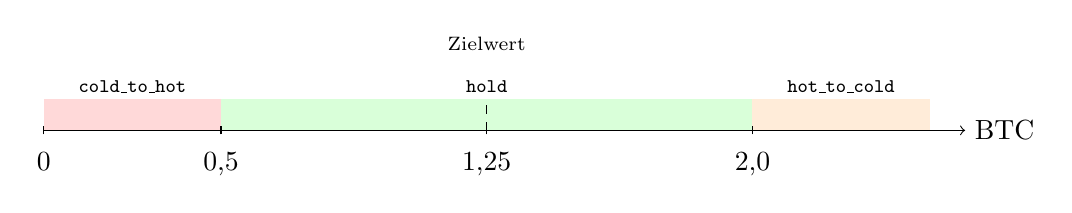
\begin{tikzpicture}[xscale=4.5]
  \fill[red!15]    (0,0)   rectangle (0.5,0.4);
  \fill[green!15]  (0.5,0) rectangle (2.0,0.4);
  \fill[orange!15] (2.0,0) rectangle (2.5,0.4);
  \draw[->] (0,0) -- (2.6,0) node[right] {\ac{BTC}};
  \foreach \x/\l in {0/0, 0.5/{0{,}5}, 1.25/{1{,}25}, 2.0/{2{,}0}}
    \draw (\x,-0.05) -- (\x,0.05) node[below=6pt] {\l};
  \node at (0.25,0.55) {\scriptsize\texttt{cold\_to\_hot}};
  \node at (1.25,0.55) {\scriptsize\texttt{hold}};
  \node at (2.25,0.55) {\scriptsize\texttt{hot\_to\_cold}};
  \draw[dashed] (1.25,0) -- (1.25,0.4) node[above=14pt] {\scriptsize Zielwert};
\end{tikzpicture}
\caption{Balance-Zonen des Hot-Wallets und resultierende \ac{OPA}-Aktionen.\\Quelle: Eigene Darstellung.}
\label{fig:balance_zonen}
\end{figure}

Beide Austausch-Transaktionen stellen ein Risiko für das Gesamtsystem dar. Wird ein \texttt{hot\_to\_cold}-Intent ausgelöst, lagert das Hot-Wallet zu viele Geldmittel und stellt einen höheren Schaden bei Kompromittierung dar. Bei einem \texttt{cold\_to\_hot}-Austausch besitzt das Hot-Wallet nur geringe Geldmittel, und die Operationalität des automatischen Transaktionssystems, also das Schutzziel der Verfügbarkeit, ist gefährdet.

Basierend auf der Aktion werden daraufhin die Ziel- und Ursprungsadresse festgelegt. Die Höhe der zu sendenden Mittel wird in Relation zum Mittelwert des optimalen Bereichs bestimmt, sodass möglichst wenige Austausch-Transaktionen zwischen Hot- und Cold-Wallet ausgeführt werden müssen.

Zudem wird ein Risk Score auf Basis des Abstands zur äußeren Grenze des optimalen Bereichs bestimmt, welcher verwendet wird, um die \ac{PSBT}-Parameter auf Basis einer gewissen Wichtigkeit oder Risikos zu bestimmen. (siehe Tabelle~\ref{tab:OPA_fundSwitch}).
\begin{table}[htbp]
\centering
\begin{tabular}{l c c c}
\toprule
\textbf{\ac{PSBT}-Parameter} & \textbf{Score $\le 30$} & \textbf{$30 <$ Score $\le 70$} & \textbf{Score $> 70$} \\
\midrule
Confirmation Blocks & 6 & 3 & 1 \\
Estimate Mode & economical & conservative & conservative \\
\bottomrule
\end{tabular}
\caption{\ac{OPA}-Kontostand-Evaluation (Parameter nach Risk Score)}
\label{tab:OPA_fundSwitch}
\end{table}

Da diese Transaktionen einen abnormalen Zustand des Basis-Systems revidieren sollen und die Parameter selbst vom System gewählt werden, wird von einer weiteren Bestätigung von \ac{PSBT}-Parametern wie \ac{BTC}-Anzahl und Gebühren durch den \ac{OPA}, wie bei normalen \acp{TX}, abgesehen. Nichtsdestotrotz wird das korrekte Funktionieren des Systems über das Vorhandensein der obligatorischen Parameter der \ac{PSBT} validiert (siehe oben).


\paragraph{Signierer} \mbox{}\\
Die gebaute und bestätigte \ac{PSBT} wird anschließend über die Middleware an den Key-Holder weitergeleitet.
Da das Schlüsselmaterial selbst die sicherheitskritischste Komponente darstellt, wurde dieser auf eine weitere \ac{VM} ausgelagert.

Wie die übrigen Schlüsselhalter-\acp{VM} basiert diese auf NixOS mit der beschriebenen Härtung (siehe Tabelle~\ref{tab:nixos_hardening}), ist jedoch im Unterschied zu den nachfolgend vorgestellten Cold-\acp{VM} weiterhin mit dem Internet verbunden.
Diese Entscheidung dient nicht dem Beobachten der Blockchain oder anderen Bitcoin-Operationen, sondern dem Aufbau einer Kommunikationsbrücke zum Haupt-System. Im realen Nachbau durch den Mandanten kann diese durch ein \ac{USB}- oder \ac{LAN}-Kabel ersetzt werden. Eine Substitution durch eine Hardware-Wallet bietet sich nicht an, da die Automatisierung des Signierungsprozesses verloren ginge.

\textbf{Internet-Verbindung} \\
Eine besondere Härtung der Internet-Verbindung wurde durch die Regeln einer nftables-Konfiguration und die Verwendung von WireGuard erreicht. Dabei werden alle Ports außer \ac{UDP} 51820 für \ac{WG} geblockt und aller Verkehr über den verschlüsselten WireGuard-Tunnel geleitet. Dieser Tunnel wird für die \ac{HTTP}-\ac{API}-Kommunikation zwischen Basis-System und Key~A verwendet.
Zudem wird \texttt{egress} während des \texttt{\seqsplit{docker compose build}}-Befehls über die nftables-Konfiguration \texttt{\seqsplit{nftables-setup.conf}} erlaubt, nach dem Build jedoch final über \texttt{\seqsplit{nftables-locked.conf}} wieder entfernt und gehärtet.

Die Erreichbarkeit der Key~A \ac{VM} ausschließlich über WireGuard wird nicht allein durch die \texttt{nftables}-Regeln auf Betriebssystemebene sichergestellt, sondern zusätzlich auf Ebene der Container-Orchestrierung erzwungen. Da Docker für veröffentlichte Ports eigene \ac{NAT}-Weiterleitungsregeln anlegt, die unabhängig von der \texttt{input}/\texttt{output}-Policy der Firewall wirken, publiziert kein Container einen Port nach außen. Stattdessen übernimmt ein dedizierter, schlanker Reverse-Proxy-Container die externe Anbindung und bindet sich ausschließlich an die statische WireGuard-Interface-Adresse \texttt{10.10.0.2}. Die Container kommunizieren ausschließlich über das interne, nicht nach außen exponierte Docker-Netzwerk und adressieren sich dabei weiterhin gegenseitig über ihre jeweiligen Service-Namen. Auf der physischen Netzwerkschnittstelle existiert dadurch zu keinem Zeitpunkt ein Dienst, der unabhängig vom WireGuard-Pfad erreichbar wäre.

\label{sec:HMAC}
Neben der In-Transit-Verschlüsselung wird ebenfalls ein privater \ac{HMAC}-Schlüssel beim \ac{HTTP}-Call eingesetzt, um die Integrität und Authentizität der Kommunikation zwischen den Systemen sicherzustellen.
Jede Anfrage an die Signier-Schnittstelle führt dazu neben der eigentlichen \ac{PSBT} drei zusätzliche Header mit: einen Zeitstempel, eine Nonce sowie die \ac{HMAC}-Signatur \cite{HMAC, rfc2104}.
Die Signatur wird über die Kombination aus Zeitstempel, Nonce und Request-Body gebildet, sodass jede nachträgliche Veränderung an einem dieser Bestandteile zur Ungültigkeit der Signatur führt.
Der Zeitstempel ist nur für einen kurzen Zeitraum gültig, sodass ältere Anfragen abgewiesen werden. In Verbindung mit der nachgelagerten Eindeutigkeitsprüfung der \ac{PSBT} (siehe Deduplizierung) wird so das Zeitfenster für ein etwaiges Wiedereinspielen abgefangener Anfragen stark eingegrenzt und die Authentizität jedes einzelnen Signierauftrags sichergestellt.

Zudem wird die Kompromittierungsgefahr für den Schlüssel-Halter weiter reduziert, da ausschließlich \acp{PSBT} angenommen werden.
Bevor eine empfangene \ac{PSBT} signiert wird, durchläuft sie eine strukturelle Policy-Prüfung, welche sicherstellt, dass ausschließlich wohlgeformte und plausibel aufgebaute Transaktionen den Signiervorgang erreichen. Geprüft wird dabei, ob die \ac{PSBT} überhaupt eine Transaktion enthält und mindestens einen Input besitzt, ob jeder Input über ein \texttt{witness\_utxo} sowie die zugehörigen \ac{BIP}32-Ableitungspfade verfügt und ob jeder Output einen gültigen Betrag größer Null aufweist.
Schlägt eine dieser Prüfungen fehl, wird die Signierung abgebrochen und die \ac{PSBT} zurückgewiesen.
Diese Prüfung ersetzt keine vollständige fachliche Transaktionsprüfung, welche im Basissystem durch Bitcoin Core und den Open Policy Agent erfolgt, verhindert aber bereits auf dem Signierer strukturell ungültige oder unvollständige \acp{PSBT} und reduziert damit die Angriffsfläche des sicherheitskritischen Signiervorgangs.

\textbf{Deduplizierung} \\
Zur Verhinderung einer mehrfachen Verarbeitung identischer Transaktionen wird jede \ac{PSBT} über ihre eindeutige \ac{PSBT}-\ac{ID} erfasst. Diese \ac{ID} wird in der Datenbank des Signers als eindeutiger Schlüssel geführt, sodass das System bereits gesehene Signiervorgänge zuverlässig erkennt. Trifft eine \ac{PSBT} mit einer bereits bekannten \ac{ID} ein, wird sie nicht erneut signiert, sondern mit der Statusmeldung \texttt{\seqsplit{ALREADY\_PROCESSED}} quittiert. Dieser Mechanismus stellt den eigentlichen, zustandsbehafteten Schutz gegen das Wiedereinspielen vollständiger Signieraufträge dar und ergänzt die zeitfensterbasierte Prüfung aus Zeitstempel und Nonce um eine dauerhafte, nachvollziehbare Eindeutigkeitsgarantie. Die Nonce jeder Anfrage wird dazu für die Dauer des Gültigkeitsfensters in einem Redis-Speicher als verwendet vermerkt, sodass eine erneut eingespielte Anfrage mit identischer, noch gültiger Nonce bereits vor der Signierung abgewiesen wird.

\textbf{Velocity-Cap (zweistufige Abflussbegrenzung)} \label{sec:keyA_vel} \\
Der maximale Geldabfluss des Hot-Wallets ist an zwei voneinander unabhängigen Punkten begrenzt. Die erste Schranke bildet das oben beschriebene tägliche Limit des \ac{OPA} im Basis-System (siehe \ref{sec:OPA_vel}). Die zweite Schranke ist ein harter, vom Basis-System unabhängiger Velocity-Cap auf der Key~A \ac{VM}.
Der Signierer führt in einem Redis-Speicher ein rollierendes Zeitfenster (Standard 24\,Stunden, \texttt{\seqsplit{VELOCITY\_WINDOW\_SEC}}) über den bereits signierten Abfluss. Dementsprechend weist dieser eine Anfrage mit \ac{HTTP}~429 ab, sobald die Summe den konfigurierten Grenzwert (Standard 40\,000\,000~\ac{SATS}, \texttt{\seqsplit{VELOCITY\_CAP\_SATS}}) überschreiten würde.

Gezählt wird ausschließlich der Nicht-Change-Abfluss über Single-Signatur-Inputs.
\acp{PSBT} mit Multi-Signatur-Input (\texttt{cold\_to\_hot}-Nachbefüllungen) werden am Witness-Script herausgerechnet, während Wechselgeld-Rückgaben an die eigene Wallet über den Master-Fingerprint erkannt werden.

Die Beweggründe und Sicherheitsbetrachtung der gestaffelten Schranken und ihr Wertverhältnis werden weiter in der Sicherheitsbetrachtung diskutiert (siehe \ref{sec:doppelter_velocity}).

\textbf{In-Transit-Tresor} \label{sec:in_transit_vault} \\
Das System verwendet einen sogenannten \emph{In-Transit-Signer}-Ansatz, bei dem ausschließlich über \acp{PSBT} kommuniziert wird und das Schlüsselmaterial das System zu keinem Zeitpunkt verlässt.
Vorhandene Alternativen für den Signierer als selbstgebauten Microservice lassen sich in \texttt{Web3Signer} von ConsenSys und \texttt{HashiCorp Vault} finden. \texttt{HashiCorp Vault} unterstützt in seiner eingebauten Signier-Engine die secp256k1-Kurve des Bitcoin-Algorithmus nicht nativ und könnte nur mit einer Erweiterung durch Plug-ins für unsere Anforderung verwendet werden \cite{vault_plugin_ethsign, vault_issue3846, sec2}.
\texttt{Web3Signer} unterstützt die secp256k1-Kurve zwar nativ, ist jedoch ausschließlich auf das Signieren von Ethereum-Transaktionen und Validator-Daten ausgelegt und kennt das für Bitcoin verwendete \ac{PSBT}-Format nicht. Eine Nutzung hätte somit eine vollständig eigene Übersetzungsschicht zwischen Bitcoin-Transaktionsformat und generischem Signieren erfordert \cite{web3signer_docs}.
Andere proprietäre Lösungen, die Bitcoin nativ unterstützen, wie \texttt{AWS KMS} oder \texttt{Google Cloud KMS} \cite{gcp_kms_algorithms}, standen nicht zur Verfügung, da das System als eigenständige, nicht an einen externen Cloud-Dienst gebundene Lösung konzipiert ist. Aufgrund dessen wurde sich für ein eigenes System entschieden. Außerdem hätte das Verwenden einer vorgefertigten Lösung die Idee des Selbstentwurfs eines besonders sicheren Systems im Zuge der Aufgabenstellung zunichtegemacht.

\textbf{TPM} \\
Das Schlüsselmaterial wird zudem besonders gesichert und nur über das \ac{TPM} entschlüsselt. Diese Technologie speichert das Geheimnis in einem speziellen Hardware-Chip und verspricht dadurch Auslese-Sicherheit \cite{TPM}.
Das \ac{TPM} wird zudem über \ac{PCR} in einem speziellen sogenannten \texttt{measured boot} versiegelt. Diese sind spezielle, zur Laufzeit nicht frei beschreibbare Register im \ac{TPM} und werden während des Boot schrittweise mit kryptographischen Hashes der geladenen Komponenten wie Firmware, Bootloader, Kernel und Konfiguration \enquote{erweitert}. Jeder neue Messwert wird mit dem bisherigen Registerinhalt verkettet und neu gehasht, sodass der Endzustand eines Registers den gesamten gemessenen Boot-Pfad eindeutig abbildet. Ein Geheimnis lässt sich an bestimmte \ac{PCR}-Werte binden und darüber versiegeln. Das \ac{TPM} gibt es nur frei, wenn dieselben Register zum Entsiegelungszeitpunkt exakt denselben Zustand aufweisen.
In einer Autorisierungs-Session wird ein während des Boots gebildetes Abbild dieses Maschinenzustands für die Versiegelung des Geheimnisses verwendet. Der Chip kann dementsprechend nur durch Verifizierung desselben Systemzustands in einer weiteren Auth-Session entsiegelt werden, was eine Kompromittierung des Schlüsselmaterials über den Schlüssel selbst ausschließt.

Die konkrete Belegung der Register wurde nicht angenommen, sondern auf der Signierer-\ac{VM} mit \texttt{systemd-analyze pcrs} empirisch erhoben (siehe Abbildung \ref{fig:PCR_belegung} im Anhang). Dabei zeigte sich, dass \ac{PCR}~8 und~11 auf dem eingesetzten Boot-Stack unerweitert bleiben (Wert \texttt{0x00\dots{}0}) und daher keine Schutzwirkung entfalten. \ac{PCR}~8 wird nur vom GRUB-Bootloader belegt, während das hier verwendete \texttt{systemd-boot} die Kernel-Befehlszeile in \ac{PCR}~12 misst. Dazu setzt \ac{PCR}~11 ein Unified Kernel Image voraus, das im Labor nicht eingesetzt wird. Die Bindung der Entsiegelung erfolgt daher an die real belegten und über Neustarts stabilen Register \ac{PCR}~4, 9 und~12:
\begin{itemize}
    \item \textbf{\ac{PCR}~4 (Boot Manager Code):} Misst den verwendeten Bootloader sowie das geladene Kernel-Image und verhindert, dass ein Angreifer einen modifizierten Bootloader oder Kernel unterschiebt.
    \item \textbf{\ac{PCR}~9 (Kernel Image und Initrd):} Speichert die kryptografischen Hashes des Linux-Kernel-Images und der initialen RAM-Disk und stellt unter NixOS sicher, dass exakt die über die Systemkonfiguration definierte Kernel-Umgebung geladen wurde.
    \item \textbf{\ac{PCR}~12 (Kernel Command Line / Boot-Konfiguration):} Erfasst unter \texttt{systemd-boot} die vollständige Kernel-Befehlszeile und die gewählte Boot-Eintrags-Konfiguration; dadurch werden manipulierte Boot-Parameter, etwa zur Umgehung der Härtung, erkannt.
\end{itemize}

Die Entsiegelung erfordert eine analoge Policy-Session, in der das \ac{TPM} die aktuellen Registerwerte prüft und das versiegelte Geheimnis \emph{in Form der 32-Byte-Entropie} nur bei exakter Übereinstimmung freigibt. Zu beachten ist, dass \acp{PCR} ausschließlich beim Systemstart gemessen und zur Laufzeit eingefroren werden, wobei eine veränderte Konfiguration erst erkannt wird, sobald sie durch einen Neustart wirksam wird. Der Schutz richtet sich damit gezielt gegen zwei Angriffe. Zum einen ist das versiegelte Geheimnis kryptografisch an den Storage-Root-Key des konkreten \ac{TPM} gebunden und lässt sich auf keinem anderen \ac{TPM} laden, sodass ein Aus- und Wiedereinbau der Hardware in ein fremdes System das Schlüsselmaterial nicht preisgibt (siehe Abbildung~\ref{fig9:tpm_pcr}). Zum anderen führt eine nachträgliche Schwächung der Härtung, etwa über ein \texttt{nixos-rebuild switch}, das Kernel oder Boot-Parameter verändert, beim nächsten Boot zu abweichenden \ac{PCR}-Werten. Daraufhin würde die Entsiegelung fehlschlagen und der Seed bleibt versiegelt. Gegen einen Angreifer, der bereits zur Laufzeit über Root-Rechte auf dem provisionierten System verfügt, schützt die \ac{PCR}-Bindung hingegen nicht. Auf dieser Ebene greifen die Netzwerkisolation und die Prozess-Härtung des Signers \cite{TPM_PRC_NixOS, tcg_tpm2}.

Da dieselbe Bindung auch legitime Änderungen an Kernel oder Boot-Konfiguration erfasst, muss der Seed nach einem bewussten System-Update erneut versiegelt werden. Dieser Schritt ist fester Bestandteil des Update-Vorgehens der Signierer-\ac{VM}.

\begin{figure}[htbp]
    \centering
    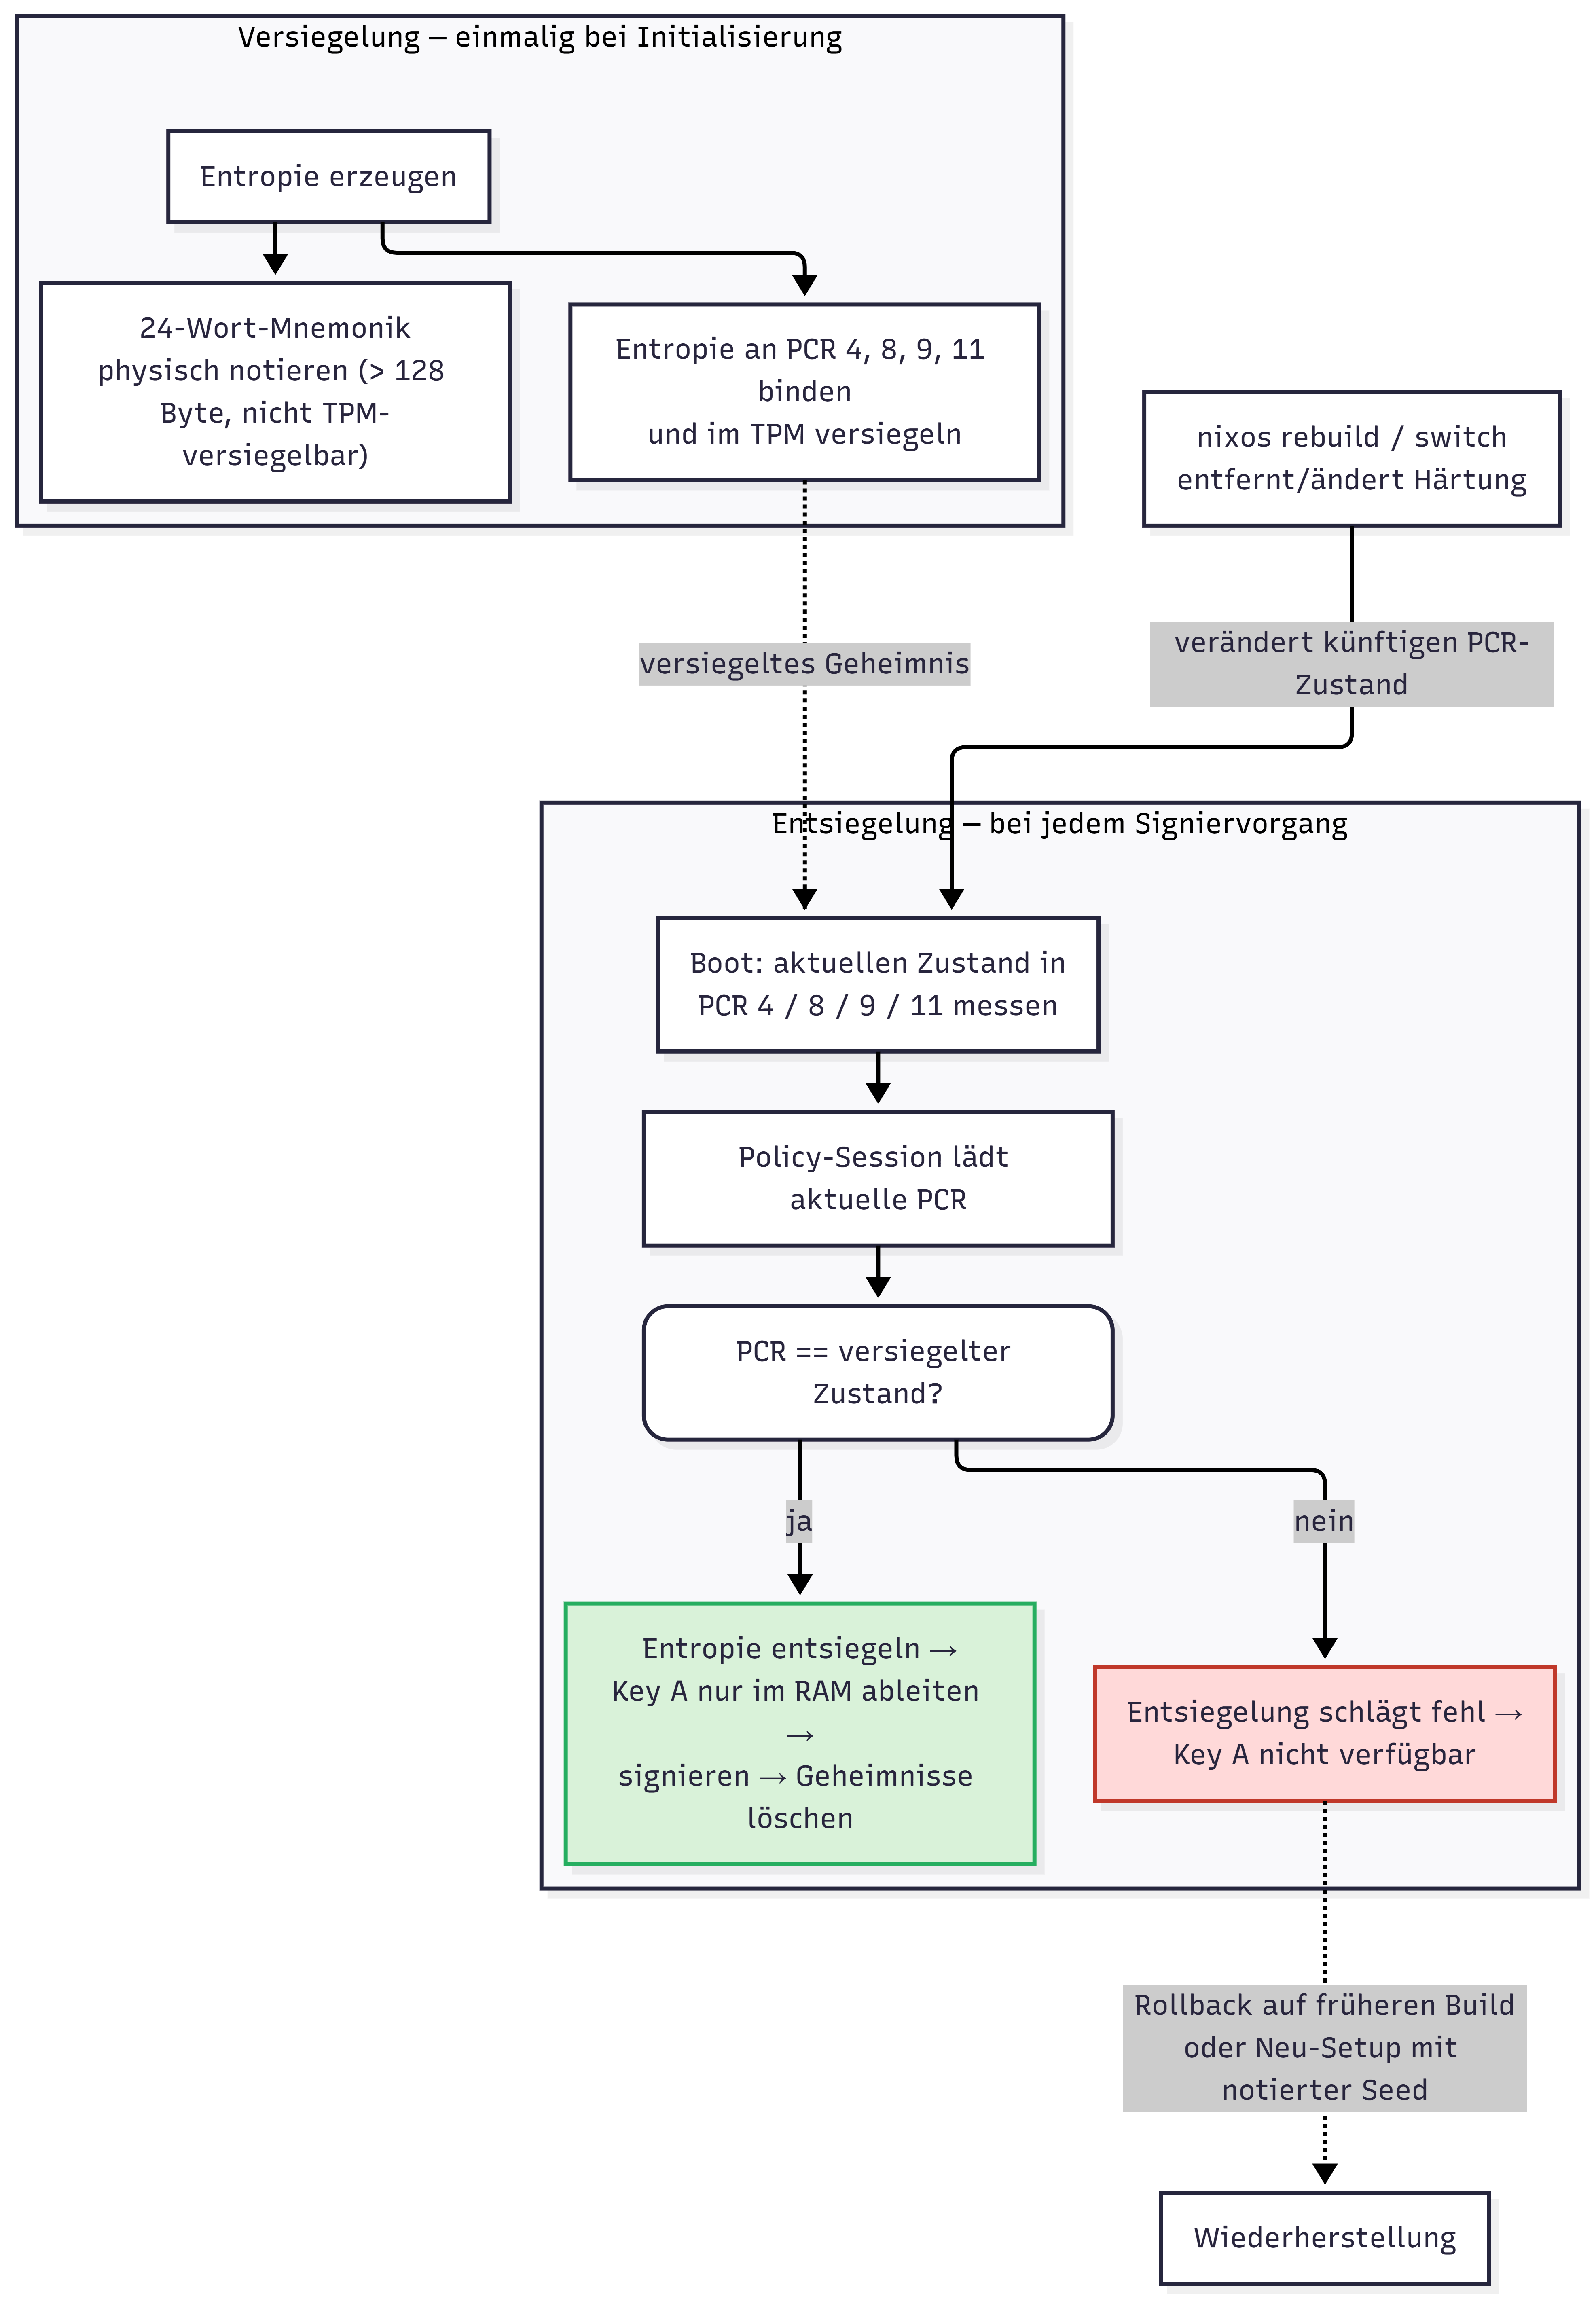
\includegraphics[width=0.98\textwidth]{Doku/Abbildungen/TPM_PCR.png}
    \caption{Darstellung der TPM-Sicherungslogik. Quelle: Eigene Darstellung.}
    \label{fig9:tpm_pcr}
\end{figure}

Die Durchsetzung der Bindung wurde geprüft, indem ein gebundenes Register zur Laufzeit künstlich mit \texttt{tpm2\_pcrextend} verändert und anschließend die Entsiegelung versucht wurde; diese schlug erwartungsgemäß fehl. Ein vollständiger \texttt{nixos-rebuild}-Test entfällt, da die Signierer-\ac{VM} bewusst keinen ausgehenden Netzzugang für den Bezug der Build-Abhängigkeiten besitzt.

Das Schlüsselmaterial bildet sich in diesem Ansatz aus der Entropie, welche als Seed im \ac{TPM} versiegelt und deren 24 mnemonische Wörter zur Sicherung in eine Datei auf dem Desktop ausgegeben werden. Diese 24 Wörter müssen für eine spätere Wiederherstellung vom Mandanten sicher notiert und die Datei anschließend über das automatisierte Skript \path{scripts/delete_seed.sh} kontrolliert entfernt werden. Empfehlungen wurden bereits in Abschnitt \ref{sec:seed_notieren} gegeben. Dementsprechend muss bei jedem Signierungsprozess die Entropie entschlüsselt und der private Schlüssel zum Signieren abgeleitet werden. Dabei wurde exakt auf die Löschung nicht benötigter Geheimnisse geachtet. Die Schlüssel selbst werden nur in den \ac{RAM} geladen und niemals auf der Festplatte gespeichert.
Eine andere Möglichkeit, dies zu realisieren, wäre, das \ac{TPM} anzuweisen, das Schlüsselmaterial intern zu generieren und nur private Schlüssel zum Signieren auszugeben, wodurch das Root-Schlüsselmaterial maximal geschützt wäre. Diese Implementation war leider nicht möglich, da das auf Proxmox virtualisierte \ac{TPM} die secp256k1-Kurve des Bitcoin-Algorithmus nicht unterstützte. Da dies ebenfalls im Fall der Hardware des Mandanten nicht garantiert werden kann, wurde sich gegen diese Umsetzung entschieden.

\textbf{Docker-Härtung} \\
Der Signer-Container, welcher als einziger Dienst unmittelbar mit angreiferkontrollierten \ac{PSBT}-Daten in Berührung kommen könnte, wurde zusätzlich auf Prozessebene gehärtet. Der Containerprozess wird unter einer dedizierten, nicht privilegierten Benutzerkennung ausgeführt und besitzt keine erweiterten Linux-Capabilities, da für den Betrieb des Signers keine davon benötigt wird: Der Zugriff auf den \ac{TPM}-Chip erfolgt über gewöhnliche Dateioperationen auf das Gerät. Die hierfür erforderliche Gerätegruppen-Zugehörigkeit wird beim Start automatisiert anhand des tatsächlichen Systemzustands ermittelt und dem Container zugewiesen. Ergänzend ist dem Prozess die Rechteausweitung über privilegierte Programmbits untersagt, und das Wurzeldateisystem des Containers ist unveränderlich eingebunden. Schreibvorgänge sind ausschließlich innerhalb der ohnehin für Wallet- und \ac{TPM}-Daten vorgesehenen, separat eingebundenen Datenverzeichnisse sowie eines flüchtigen Arbeitsspeicherbereichs für temporäre Dateien möglich. Eine erfolgreiche Kompromittierung des Signiervorgangs, etwa über einen Fehler beim Parsen einer \ac{PSBT}, bliebe dadurch auf die minimalen Rechte eines einzelnen, nicht privilegierten Prozesses beschränkt und führte nicht zu einer Rechteausweitung auf Betriebssystemebene.

Ein automatisiertes Skript \path{wgHMAC_export.sh} zum Extrahieren der Wallet-Informationen samt \ac{xpub}, Public-Deskriptor und \seqsplit{Meta-Informationen} auf einen \ac{USB}-Stick wurde implementiert und hilft dem Mandanten beim Aufsetzen des Whitelistings auf der Hot-Wallet-\ac{VM} sowie beim Hinzufügen des \ac{xpub} im Multi-Signatur-Verfahren des Cold-Wallets.
Dieses Skript schreibt gleichzeitig das \ac{HMAC}-Geheimnis und die WireGuard-Konfiguration samt Public Key~Auf diesen \ac{USB}-Stick. 
Diese Informationen können daraufhin per \ac{SSH} in das Dateiverzeichnis des Basis-Systems geladen werden und anschließend  per automatisiertem Skript auf der Hot-Wallet eingespielt werden, was das Laden der Deskriptoren in die PostgreSQL-\ac{DB} und das Pflegen der Geheimnisse in die \path{env.runtime} des Middleware-Docker-Containers umfasst (siehe~\ref{sec:SSH}).

Die für die Datenbankanbindung notwendigen Zugangsdaten werden nicht statisch vorgegeben, sondern bei der Erstinitialisierung der Key~A \ac{VM} automatisiert und zufällig erzeugt. Sie verbleiben dabei außerhalb der versionierten Konfiguration in einer separaten, restriktiv berechtigten Laufzeitdatei, auf welche ausschließlich die beteiligten lokalen Prozesse Zugriff erhalten. In Verbindung mit der bereits beschriebenen Netzwerkisolation, durch welche die Datenbank ebenfalls keinen nach außen gerichteten Port mehr besitzt, wird damit ausgeschlossen, dass über einen direkten Datenbankzugriff von außen die \ac{ID}-basierte Eindeutigkeitsprüfung bereits verarbeiteter \acp{PSBT} umgangen werden könnte.

Ausgegeben werden nach den beiden Abläufen \acp{PSBT} für den Nachfüll-Prozess sowie finalisierte Hot-\acp{TX} für das vollautomatisierte Hot-Wallet.

Eine tiefere Beschreibung der Konfiguration und des gesamten Setup- und Signierungsprozesses kann in der \path{README.md} des NixOsHot- und Basis-System-GitHub nachgelesen werden \cite{NixOsHot_github, Krypto_Basis_github}. Eine Kurzübersicht aller Skripte bietet Tabelle~\ref{tab:skripte} im Anhang.

\subsection{Cold-Wallet}

Das Cold-Wallet ist vollständig air-gapped und besitzt keinerlei Netzwerkverbindung. Die Systeme werden auf dedizierten virtuellen Maschinen in der Proxmox-Umgebung betrieben, deren Netzwerkfunktionen sowohl auf Betriebssystem- als auch auf Hypervisor-Ebene deaktiviert sind \cite{airgap_psbt_guide, Wallets}.

Das vom Internet isolierte Cold-Wallet bildet den architektonischen Kern des Systems und verwaltet ca.\ 95\,\% der Bitcoin-Bestände. Diese gilt es dementsprechend besonders zu schützen, weshalb sich für ein Air-Gap und ein 2-aus-3-Multi-Signatur-Wallet entschieden wurde. Die Isolierung des Systems reduziert die Angriffsfläche gegenüber netzwerkbasierten Angriffen erheblich und verhindert direkte Remote-Kompromittierungen.

Unter der Voraussetzung eines sicheren Perimeters am Standort des Mandanten verbleiben als Bedrohungen im Wesentlichen der operationelle Signierprozess selbst, der Datentransfer über das Wechselmedium sowie die Software-Lieferkette der eingesetzten Komponenten. Diese werden in der Sicherheitsbetrachtung
(siehe \ref{sec:sicherheitsbetrachtung}) einzeln bewertet.
Um den operationellen Prozess sicher zu gestalten, wurde sich für einen 2-aus-3-Multi-Signatur-Prozess entschieden, wobei über einen \ac{USB}-Stick \acp{PSBT} transferiert werden können \cite{riskpublishing_hotcold,bip174,Sparrow_Wallets_Best_Practices,knowingbitcoin_hotcold,psbt_dcentral,airgap_psbt_guide}.
Dieser Multi-Signatur-Prozess wird besonders für hohe Geldsummen und professionelle Architekturen empfohlen und findet dementsprechend Verwendung \cite{Sparrow_Wallets_Best_Practices}. Ein Hinzufügen weiterer benötigter Signaturen durch einfaches Ergänzen zusätzlicher Cold-\acp{VM} und das Erhöhen des Reglers bleibt im Ermessen des Mandanten.

\subsubsection{Architektur}

\paragraph{Hardware und Betriebssystem} \mbox{}\\
Die Aufteilung auf zwei getrennte \acp{VM} (Key~B und Key~C) ergibt sich unmittelbar aus dem 2-aus-3-Multi-Signatur-Modell. Zusammen mit dem im Hot-System gehaltenen Key~A bilden sie drei unabhängige Cosigner, von denen zwei zur Freigabe einer Cold-Transaktion genügen. 
Die physische Trennung auf zwei Maschinen verhindert, dass die Kompromittierung eines einzelnen Cold-Systems bereits zwei Schlüssel preisgibt. Key~C dient zusätzlich als Recovery-Schlüssel (siehe~\ref{sec:backup}), sodass, wenn eine Maschine ausfällt, die Spend-Fähigkeit über die verbleibenden zwei Schlüssel erhalten bleibt und die gesamten Assets auf ein neues Wallet transportiert werden können. Der Mandant kann die beiden \acp{VM} an getrennten, physisch gesicherten Orten betreiben oder das Verfahren durch weitere Cold-Signer auf ein 3-aus-4-Schema verschärfen.

Als air-gap-fähiger Multi-Signatur-Koordinator und Schlüsselhalter der Cold-\acp{VM} wurde Sparrow Wallet gewählt. Ausschlaggebend waren die vollständige Offline-Fähigkeit, die transparente Darstellung der Zieladressen, \ac{TX}- und \ac{UTXO}-Details für die manuelle Verifikation (siehe \ref{sec:sparrow_signierung}) sowie die native Unterstützung von Deskriptoren und dem \ac{PSBT}-Prozess. Die konkrete Abwägung gegen die Alternativen folgt im Anschluss (siehe \ref{sec:alt_sparrow}).

Das Multi-Signatur-Wallet selbst enthält auf jeder \ac{VM} je einen geheimen kryptographischen Schlüssel und je zwei öffentliche Schlüssel (siehe \ref{sec:cold_setup}). Jeder einzelne Schlüssel bleibt isoliert, und eine manuelle Verifikation durch den Mandanten bleibt als Voraussetzung für den Broadcast bestehen.

Für die sicherheitskritische Komponente des kryptographischen Schlüsselmaterials wird NixOS als Betriebssystem verwendet. Dies ermöglicht reproduzierbare, deklarative und minimalistische Konfigurationen. Eine besondere Härtung der Hardware- und Netzwerk-Schicht sichert gegen unbeabsichtigtes Mounten von \ac{USB}-Medien und Zugriff über offene Ports ab \cite{nixos_funktionsweise}.

Auf diesem System wird NixOS bewusst so konfiguriert, dass bestimmte nutzerfreundliche Funktionen bereitgestellt werden, die nicht Teil einer Standard-NixOS-Installation sind. Ziel ist es, sicherheitskritische Skripte kontrolliert und dennoch einfach nutzbar zu machen.
Darunter fallen ein deklarativer Desktop-Mount sowie automatisierte Skripte. Zudem führt der \ac{XFCE}-Dateimanager (Thunar) Shell-Skripte nicht standardmäßig per Doppelklick aus. Diese Einschränkung wird explizit aufgehoben, um dem Nutzer für bestimmte Skripte eine einfachere Nutzung zu ermöglichen.

\paragraph{Sparrow Wallet} \mbox{}\\
Sparrow Wallet ist eine quelloffene Desktop-Bitcoin-Wallet mit Fokus auf Self-Custody, Sicherheit und Transparenz, womit sie die inhaltlichen Anforderungen des Mandanten unterstützt. Sie unterstützt Single- und Multi-Signatur, Output-Deskriptoren und
den vollständigen \ac{PSBT}-Prozess nach \cite{bip174}. 
Außerdem wird eine Anbindung an einen eigenen Bitcoin Core Node ermöglicht, welche wir nicht nutzen, jedoch als Alternative anerkennen (siehe \ref{sec:alt_Sparrow_broadcast}). 
Es unterstützt zudem die Besonderheit der Cold-Wallet \acp{VM}, sodass es offline Signierung sowohl über Dateien, \ac{USB} als auch animierte \ac{QR}-Codes ermöglicht. Daneben zeichnet es sich ebenfalls durch eine breite Hardware-Wallet-Integration und eine Vielzahl an Konnektoren und Wallet Formaten aus, welche als weitere Alternativen beschrieben wurden und dem Mandanten offenstehen (Siehe \ref{sec:alt_alg}).
Ein besonderes Merkmal ist die transparente Darstellung aller Transaktions- und \ac{UTXO}-Details, die die manuelle Verifikation im Cold-Prozess erst sicher und praktikabel macht und dementsprechend fest eingeplant ist (siehe \ref{sec:sparrow_signierung}) \cite{sparrow_docs,Sparrow_Wallets_Features}.

In unserer Integration fungiert Sparrow Wallet als Multi-Signatur"=Koordinator"=, \ac{PSBT}-Handler und Key Holder. Eine Instanz darf diese Rollen, wie oben bereits erwähnt, gleichzeitig halten \cite{sparrow_docs,sparrow_multisig}.
Zudem verwaltet die Applikation keine vollständige Blockchain, da sie keine Netzwerkverbindung besitzt. Private Schlüssel verbleiben ausschließlich auf den jeweiligen Cold-Key-Systemen, während allein der interne und externe Multi-Signatur-Deskriptor des Cold-Wallets auf Bitcoin Core registriert wird \cite{sparrow_multisig, airgap_psbt_guide}.

Sparrow übernimmt im Cold-Bereich folgende Aufgaben:
\begin{itemize}
  \item Import und Anzeige freigegebener \acp{PSBT},
  \item Koordination der Multi-Signatur-Signaturen,
  \item Überprüfung der Skript- und Adressstruktur,
  \item Zusammenführung und Finalisierung der Signaturen.
\end{itemize}

Anzuführen ist ebenfalls, dass sich Sparrow während der Entwicklung durch einen Fehler im stable-Release auszeichnete. Nach dem Download aus dem Nix-Store und dem Ausführen des Programms ergaben sich Probleme mit der JavaFX-Bibliothek, und verschiedene Fenster mit dem Fehler \emph{\textbf{Panes omitted}} konnten nicht angezeigt werden.
Aufgrund dessen wurde sich während der Entwicklung für die unstable-Version entschieden, die Java~25 nativ unterstützt und diese Probleme behob. Während der Entwicklung wurde zudem NixOS 26.05 veröffentlicht, welche Java~25 direkt umfasst, weshalb der unstable-channel während der Entwicklungsperiode wieder aufgehoben werden konnte.
Die Channels \texttt{nixos-stable} und \texttt{nixos-unstable} sind beide offizielle, von den NixOS-Maintainern betreute Zweige desselben Repositories. \texttt{unstable} ist dabei nicht schlechter gepflegt, sondern lediglich der schneller aktualisierte Rolling-Zweig mit neueren Paketversionen (hier Java~25), der kürzer stabilisiert wurde. Die zwischenzeitliche Nutzung von \texttt{unstable} war daher eine bewusste, temporäre Wahl zur Behebung des JavaFX-Fehlers.

Zusätzlich wird die Wallet-Anwendung deklarativ in NixOS integriert: Installation über den Nix Store, definierte Startparameter (Netzwerkmodus \texttt{-{}-regtest}) und Bereitstellung einer Desktop-Datei, welche den Start per Doppelklick auf das Desktop-Icon ermöglicht.

\label{sec:dyn_adress}
Eine Besonderheit von Bitcoin, die extra beachtet werden musste, stellt die Adressierung von Wallets dar.
Während für jede \ac{TX} dieselbe statische Empfangsadresse verwendet werden kann, stellt dies nicht den Standard dar.
Zur Verringerung der Nachvollziehbarkeit von \ac{TX}-Abläufen und damit Erhöhung des Datenschutzes werden oft Zieladressen dynamisch aus dem öffentlichen externen Deskriptor nach der \ac{BIP}32-Hierarchie gebildet.
Dies ist ebenfalls für den internen Deskriptor und die Quell-Adresse der Fall, wobei diese bereits im Signierprozess als von dieser Wallet stammend verifiziert wird und kein größeres Problem darstellt.

Dieser Sachverhalt stellt ein Problem für die manuelle Verifikation von \ac{PSBT}-Details wie im Signierungsprozess (siehe \ref{sec:cold_sign}) beschrieben dar, da die Zieladresse als zugehörig zur Hot-Wallet von Key~A verifiziert werden soll.
Dafür sollte der externe Deskriptor von Key~A als Watch-Only-Wallet integriert werden, sodass Sparrow die dynamische Adresse zu dem hinterlegten Wallet vollautomatisch auflösen kann. Der Mandant kann so direkt verifizieren, dass die Cold-Wallet-\ac{PSBT} Geld nur an das Hot-Wallet sendet. 

Die Wahl des Koordinators ist eine architektonische Grundsatzentscheidung und wird der Implementierung bewusst vorangestellt: Erst wenn feststeht, welche Software die Rollen Koordinator, \ac{PSBT}-Handler und Schlüsselhalter air-gapped vereinen kann, ergibt der konkrete Setup- und Signierprozess Sinn.
\textbf{Alternativen zu Sparrow Wallet} \label{sec:alt_sparrow} \\
Als air-gap-fähige Koordinatoren kämen ebenfalls \texttt{Electrum}, \texttt{Specter Desktop}, \texttt{Nunchuk}, \texttt{Caravan} sowie \texttt{Bitcoin Core} selbst in Frage. Diese decken jedoch jeweils nur Teile der benötigten Funktionalität netzunabhängig ab und fanden aufgrund dessen keine Verwendung.

\begin{table}[htbp]
\centering
\footnotesize
\renewcommand{\arraystretch}{1.3}
\begin{tabularx}{\linewidth}{@{} l c c >{\RaggedRight}X @{}}
\toprule
\textbf{Kandidat} & \textbf{Offline-} & \textbf{Air-gapped} & \textbf{Ausschlussgrund} \\
                  & \textbf{fähig}    & \textbf{Key-Halter} & \\
\midrule
\texttt{Electrum} & teilw. & nein
  & Online-Variante benötigt öffentlichen Electrum-Server (Metadaten-Leak),
    offline keine Wallet-übergreifende Adressauflösung, nicht Deskriptor-native
    Konventionen erschweren \path{wsh}-Interoperabilität. \\
\addlinespace
\texttt{Bitcoin Core} & ja & ja (nur Keys)
  & Kein für die manuelle Verifikation optimiertes \ac{GUI}
    (Zieladresse, Betrag, \ac{UTXO}-Flüsse). \\
\addlinespace
\texttt{Specter Desktop} & ja & nein
  & Reiner Koordinator ohne eigenes Schlüsselmaterial, nur gekoppelt mit
    Bitcoin Core nutzbar, dann größere Codebasis/Angriffsfläche und geringere
    \ac{PSBT}-Detailtiefe. \\
\addlinespace
\texttt{Nunchuk} & ja & nein
  & Auf externe Signer (Hardware/Tapsigner) ausgelegt, eigene Software-Keys
    vom Hersteller als testweise/unsicher deklariert. \\
\addlinespace
\texttt{Caravan} & ja & nein
  & Zustandslose Web-App, nur Watch-Only-Koordinator, keine Persistenz der
    Wallet-Konfiguration, rudimentäre \ac{TX}-Darstellung. \\
\midrule
\textbf{Sparrow (gewählt)} & \textbf{ja} & \textbf{ja}
  & Vereint Koordinator, \ac{PSBT}-Handler und Key-Halter offline, transparente
    \ac{TX}-/\ac{UTXO}-Anzeige für die manuelle Verifikation, native
    Deskriptor- und \ac{PSBT}-Unterstützung. \\
\bottomrule
\end{tabularx}
\caption{Bewertung air-gap-fähiger Multi-Signatur-Koordinatoren gegenüber Sparrow Wallet}
\label{tab:sparrow_alternativen}
\end{table}


\subsubsection{Sicherheitsmodell}

\paragraph{Backup und Wiederherstellung} \label{sec:backup} \mbox{}\\
Für die Wiederherstellbarkeit des Systems sind drei Artefakte relevant, die
getrennt und redundant zu sichern sind:
\begin{itemize}
    \item \textbf{Seeds:} Die 24-Wort-Phrasen aller drei Schlüssel (Key~A bis Key~C) werden ausschließlich analog verwahrt (siehe \ref{sec:seed_notieren}), idealerweise an räumlich getrennten, physisch gesicherten Orten.
    \item \textbf{Wallet-Deskriptor:} Der \path{wsh(sortedmulti(...))}-Deskriptor samt der \ac{xpub}-Fingerprints ist für die Wiederherstellung des Multi-Signatur-Wallets funktional zwingend erforderlich: Zwei Seeds allein genügen nicht, um die Wallet-Struktur und die Ableitungspfade zu rekonstruieren. Da der Deskriptor kein Geheimnis darstellt, kann er mehrfach kopiert und gemeinsam mit jedem Seed-Backup abgelegt werden.
    \item \textbf{Systemkonfiguration:} Die deklarativen NixOS-Konfigurationen samt gepinntem Flake erlauben den identischen Neuaufbau jeder \ac{VM}.
\end{itemize}
Auf dieser Grundlage sind alle relevanten Ausfallszenarien abgedeckt:
\begin{itemize}
    \item \textbf{Ausfall einer Cold-\ac{VM} (Key~B oder Key~C):} Durch das 2-aus-3-Modell bleibt die Spend-Fähigkeit über die verbleibenden zwei Schlüssel erhalten. Die ausgefallene Maschine wird aus der Konfiguration neu aufgebaut und der Schlüssel aus dem Seed-Backup wiederhergestellt. Alternativ werden die Bestände auf ein neu aufgesetztes Wallet transferiert.
    \item \textbf{Ausfall der Key~A \ac{VM} (inklusive \ac{TPM}-Defekt):} Das \ac{TPM} versiegelt lediglich die lokal vorgehaltene Entropie. Die maßgebliche Sicherung ist die analog notierte Seed-Phrase. Auf einer neu aufgebauten \ac{VM} wird der Seed eingespielt und erneut im \ac{TPM} der neuen Maschine versiegelt.
    \item \textbf{Verlust oder Defekt des Wechselmediums:} Da sich pro Zeitpunkt höchstens eine \ac{PSBT} auf dem Medium befindet und deren Zustand in der \ac{PSBT}-\ac{DB} geführt wird, geht kein Schlüsselmaterial verloren. Der betroffene Vorgang wird verworfen und neu angestoßen.
    \item \textbf{Gleichzeitiger Verlust zweier Schlüssel:} Dieser Fall ist durch die räumlich getrennte Seed-Verwahrung abzufangen und markiert die Grenze des Modells. Er ist organisatorisch, nicht technisch zu verhindern.
\end{itemize}



\paragraph{Broadcast} \mbox{}\\
Eine zusätzliche Integritätssicherung der finalisierten \ac{TX} auf dem Rückweg zum Basis-System ist nicht erforderlich. Jede nachträgliche Veränderung an Inputs, Outputs oder Beträgen invalidiert die bereits geleisteten Signaturen, sodass eine derart veränderte \ac{TX} bei der Validierung durch das Bitcoin-Netzwerk zwangsläufig abgewiesen wird. 
Auch ein vollständiger Austausch der Datei gegen eine andere, in sich gültige
\ac{TX} gefährdet die Bestände nicht: Eine fremde Transaktion trägt keine Signaturen des Cold-Wallets und kann dessen \acp{UTXO} daher nicht bewegen.
Eine Kompromittierung dieses letzten Schrittes beträfe somit ausschließlich das Schutzziel der Verfügbarkeit und der Broadcast unterbliebe oder müsste
wiederholt werden. Es zöge keinen Verlust von Assets nach sich. Gleichwohl gilt es, diesen Zustand über das Monitoring zu erkennen und zu vermeiden.

Die operativen Abläufe des Cold-Wallets, welche das einmalige Setup sowie den manuelle Signierungs-Prozess beinhalten, umfassen Komponenten beider Systeme und werden daher nach der Vorstellung der Hot-Wallet-Services gesammelt in Abschnitt~\ref{sec:prozesse} beschrieben.





\subsection{Prozesse} \label{sec:prozesse}

Nachdem alle beteiligten Services beschrieben wurden, stellt dieser Abschnitt die operativen Abläufe des Gesamtsystems dar: das einmalige Setup, den vollautomatischen Hot-Transaktionsprozess, den manuellen Operator-Pfad sowie den asynchronen Cold-Prozess mit dem zugehörigen Lebenszyklus der
Nachbefüllungs-\ac{PSBT}. 
Der Datenaustausch zwischen Online- und Offline-Systemen erfolgt ausschließlich über ein dediziertes Wechselmedium. Pro Zeitpunkt befindet sich stets nur eine Transaktion auf dem Medium, wodurch Verwechslungen und Zustandsinkonsistenzen vermieden werden.


\subsubsection{Cold-Setup} \label{sec:cold_setup}

Vorausgesetzt wird das erfolgreiche Installieren der Cold- und Hot-Wallet-NixOS-Images. Dieses Setup lädt beim Installieren von NixOS, wie bereits erwähnt, durch deklarative Statements alle nötigen Programme und Skripte auf den Desktop.
Es wird empfohlen, für die \acp{VM} von Key~B und Key~C zuerst die \ac{LAN}-Bridge von der \ac{VM} auf Hypervisor- oder Hardware-Ebene zu entfernen und anschließend Sparrow auf dem Desktop zu öffnen. Das Programm startet im Regtest-Modus, und die Variable \texttt{\seqsplit{cold.sparrowNetwork}} sollte in der Datei \path{configuration.nix} bei produktiver Nutzung auf den Wert mainnet umgestellt werden. Zu beachten ist dabei außerdem, dass bei der Umstellung auf das Mainnet sämtliche Wallets neu aufgesetzt werden müssen (siehe \ref{sec:mainnet_migration}).

Anschließend muss je \ac{VM} ein Wallet importiert oder eine neue mnemonische Phrase festgelegt werden.
\label{sec:seed_notieren}
Zur Sicherung der Seed Phrase bestehend aus 24~mnemonischen~Wörtern empfiehlt sich eine ausschließlich analoge, offline gehaltene Aufbewahrung wie handschriftlich auf Papier oder dauerhafter als in Metall gestanztes Seed-Backup an einem physisch gesicherten Ort wie einem Tresor. Die Phrase ist notwendig, um das Wallet wiederherzustellen und kann zur Erhöhung der Ausfallsicherheit in Form mehrerer Kopien an räumlich getrennten Orten verwahrt werden. Eine digitale Speicherung wie beispielsweise als Foto, in der Cloud oder in einem Passwortmanager ist zu vermeiden, da sie das Air-Gap-Prinzip unterläuft. Der Mandant kann die Phrase zusätzlich durch eine \ac{BIP}39-Passphrase ergänzen oder nach \ac{SLIP}-39 auf mehrere Anteile aufteilen.
Ein weiteres Passwort für die Verschlüsselung der Wallet in Sparrow kann festgelegt werden und ist empfohlen.

Zuletzt müssen die \ac{xpub}-Schlüssel aus Key~A und Key~C extrahiert werden, unter der Prämisse, dass Key~B und der Multi-Signatur-Koordinator auf einer Maschine zusammengelegt wurden.
Das Skript \path{wgHMAC_export.sh} kann auf der \ac{VM} von Key~A ausgeführt werden, um eine automatische Ordnerstruktur anzulegen und die Wallet-Informationen in Form einer \path{meta.json} zu extrahieren.
Dabei werden die öffentlichen Deskriptoren für die \ac{BIP}84 Ableitung (Single-Signatur) und den \ac{BIP}48 Multi-Signatur Pfad gebildet.

Der Deskriptor für das Multi-Signatur Wallet muss auf beiden \ac{VM} der Key~B und C Wallet importiert und als eine der drei Signaturen in Form eines xpub samt Fingerprint eingetragen werden.
Um ein neues Wallet für Key~B und C zu erstellen, muss je \ac{VM} \emph{eine} neue (oder bekannte) Seed Phrase eingegeben werden. Durch das Eintragen der Seed-Phrase im Multi-Signatur-Wallet Kontext wird von dieser Seed-Phrase automatisch der richtige Ableitungskontext von \path{m/48h/1h/0h/2h} (\path{1h} = Coin-Type für Testnet/Regtest, im Mainnet \path{0h}, siehe \ref{sec:mainnet_migration}) gebildet.
Die Sparrow Konfiguration wird in Abbildung \ref{fig3:sparrow_multiSetup} dargestellt.
Diese muss als neue Datei in Form ihres xpubs und Fingerprints auf das Wechselmedium kopiert werden und wie Key~A als watch-only Bestandteil auf der je anderen \ac{VM} eingetragen werden.

\begin{figure}[htbp]
    \centering
    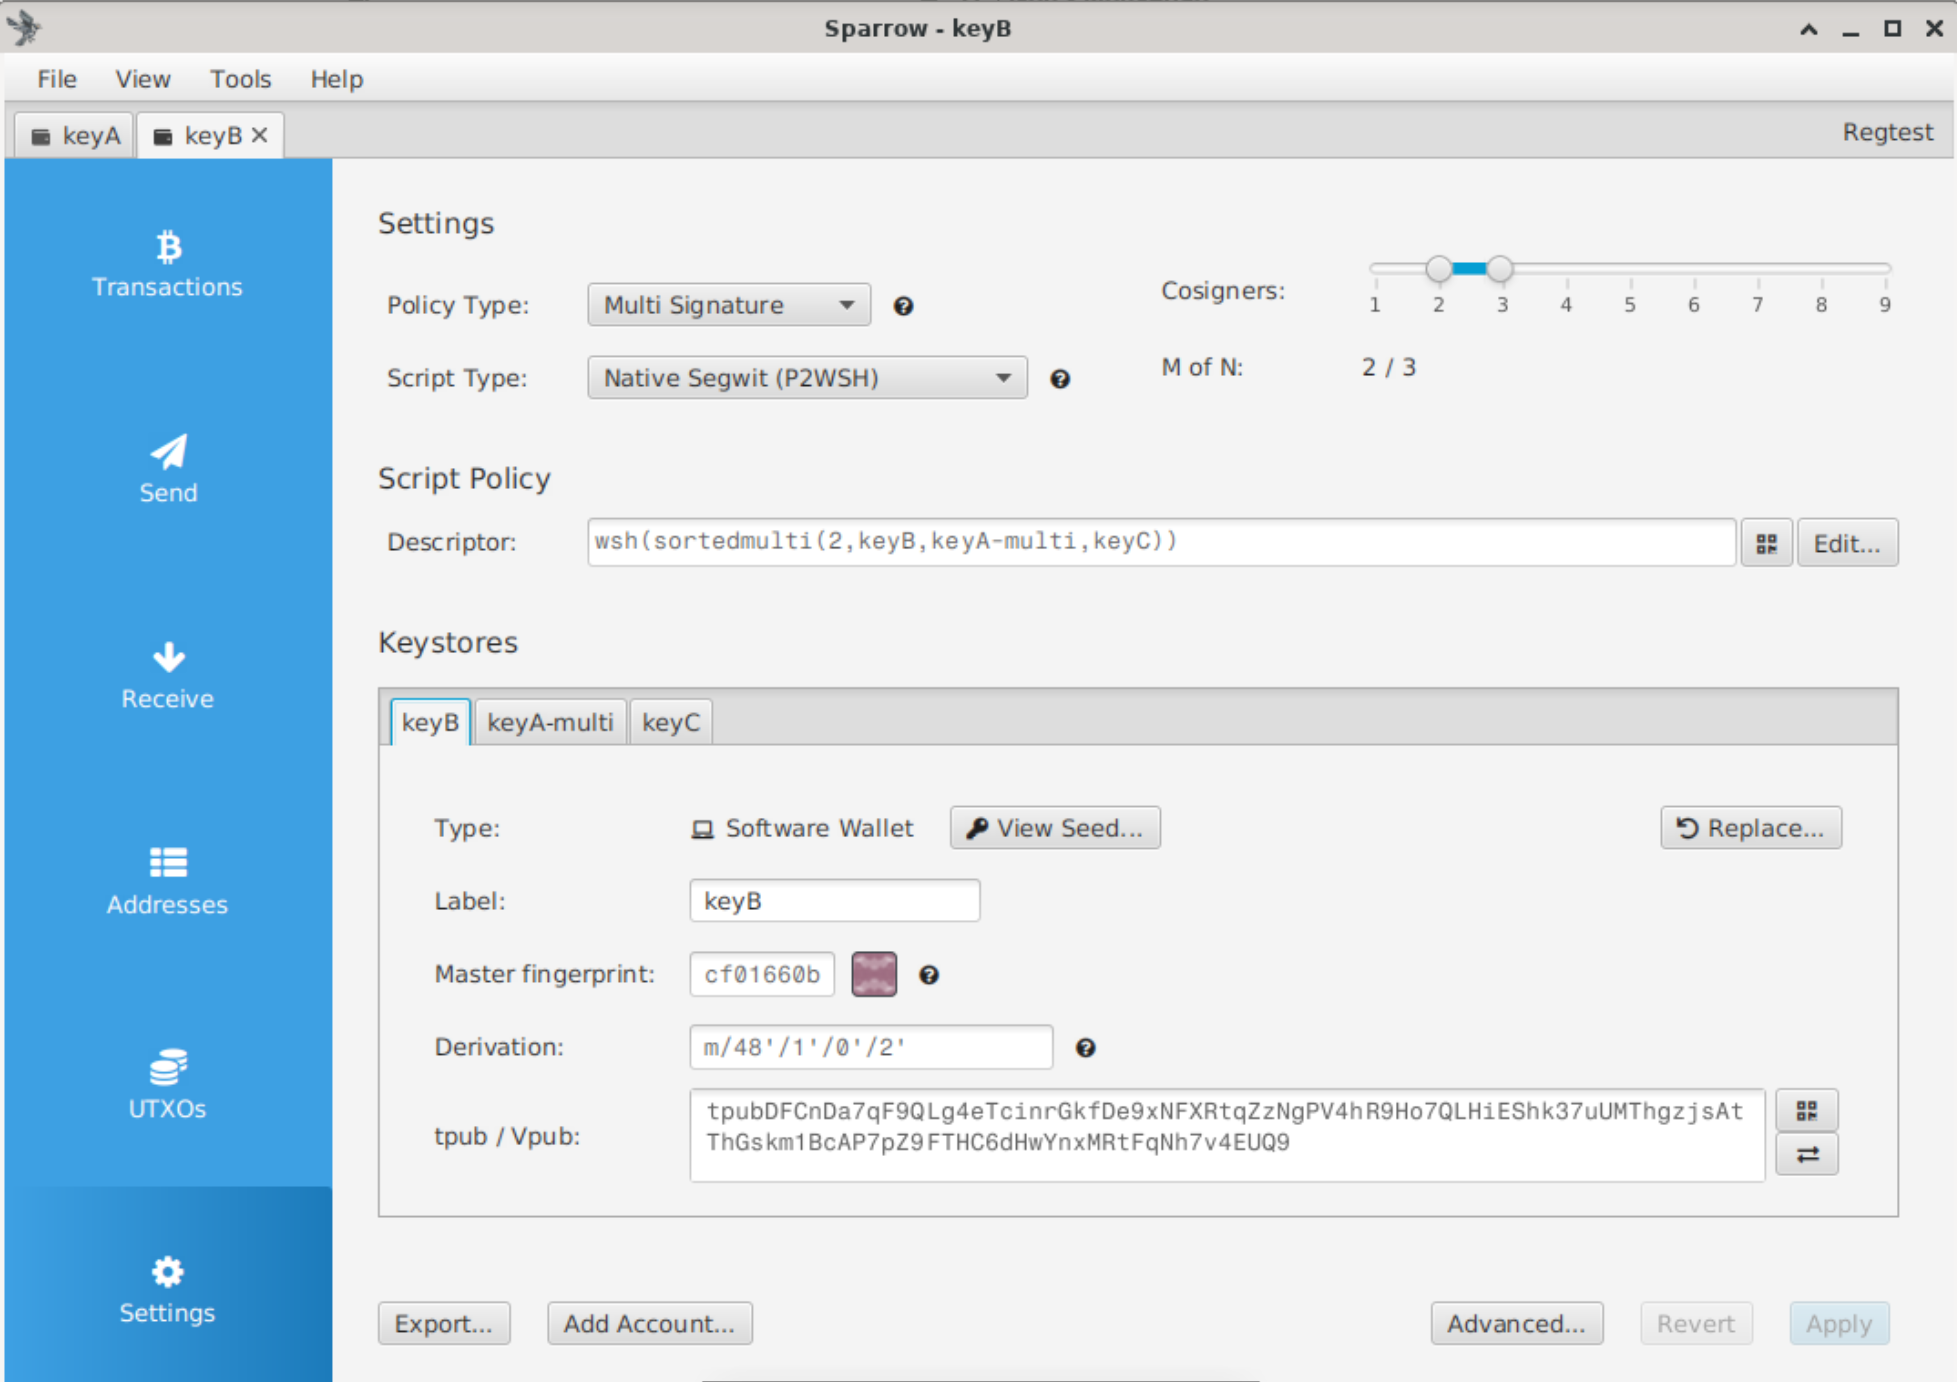
\includegraphics[width=0.8\textwidth]{Doku/Abbildungen/sparrow/sparrow_multiSetup.png}
    \caption{Sparrow Multi-Signatur - Einstellungen. Quelle: Eigenes Bildschirm-Foto aus Sparrow.}
    \label{fig3:sparrow_multiSetup}
\end{figure}

Der \ac{BIP}84 Schlüssel wird primär für das automatische Signieren für des Hot-Wallet verwendet. Es empfiehlt sich jedoch ebenfalls, diesen direkt in Sparrow als separate Watch-Only-Wallet zu registrieren. Dadurch werden dynamische Adressen, die zu diesem Wallet gehören, automatisch aufgelöst und als Zieladresse der Transaktion angezeigt. \label{sec:sparrow_keyA_load}

Der daraus generierte wsh-Deskriptor muss anschließend als separate Datei auf dem Wechselmedium unter \path{/wallets/cold} als \path{cold-signer.wsh} abgelegt werden. Durch diese Nomenklatur kann der Deskriptor im nächsten Schritt vollautomatisch auf dem Basis-System importiert werden (siehe \ref{sec:wallet_import}).

\begin{figure}[htbp]
    \centering
    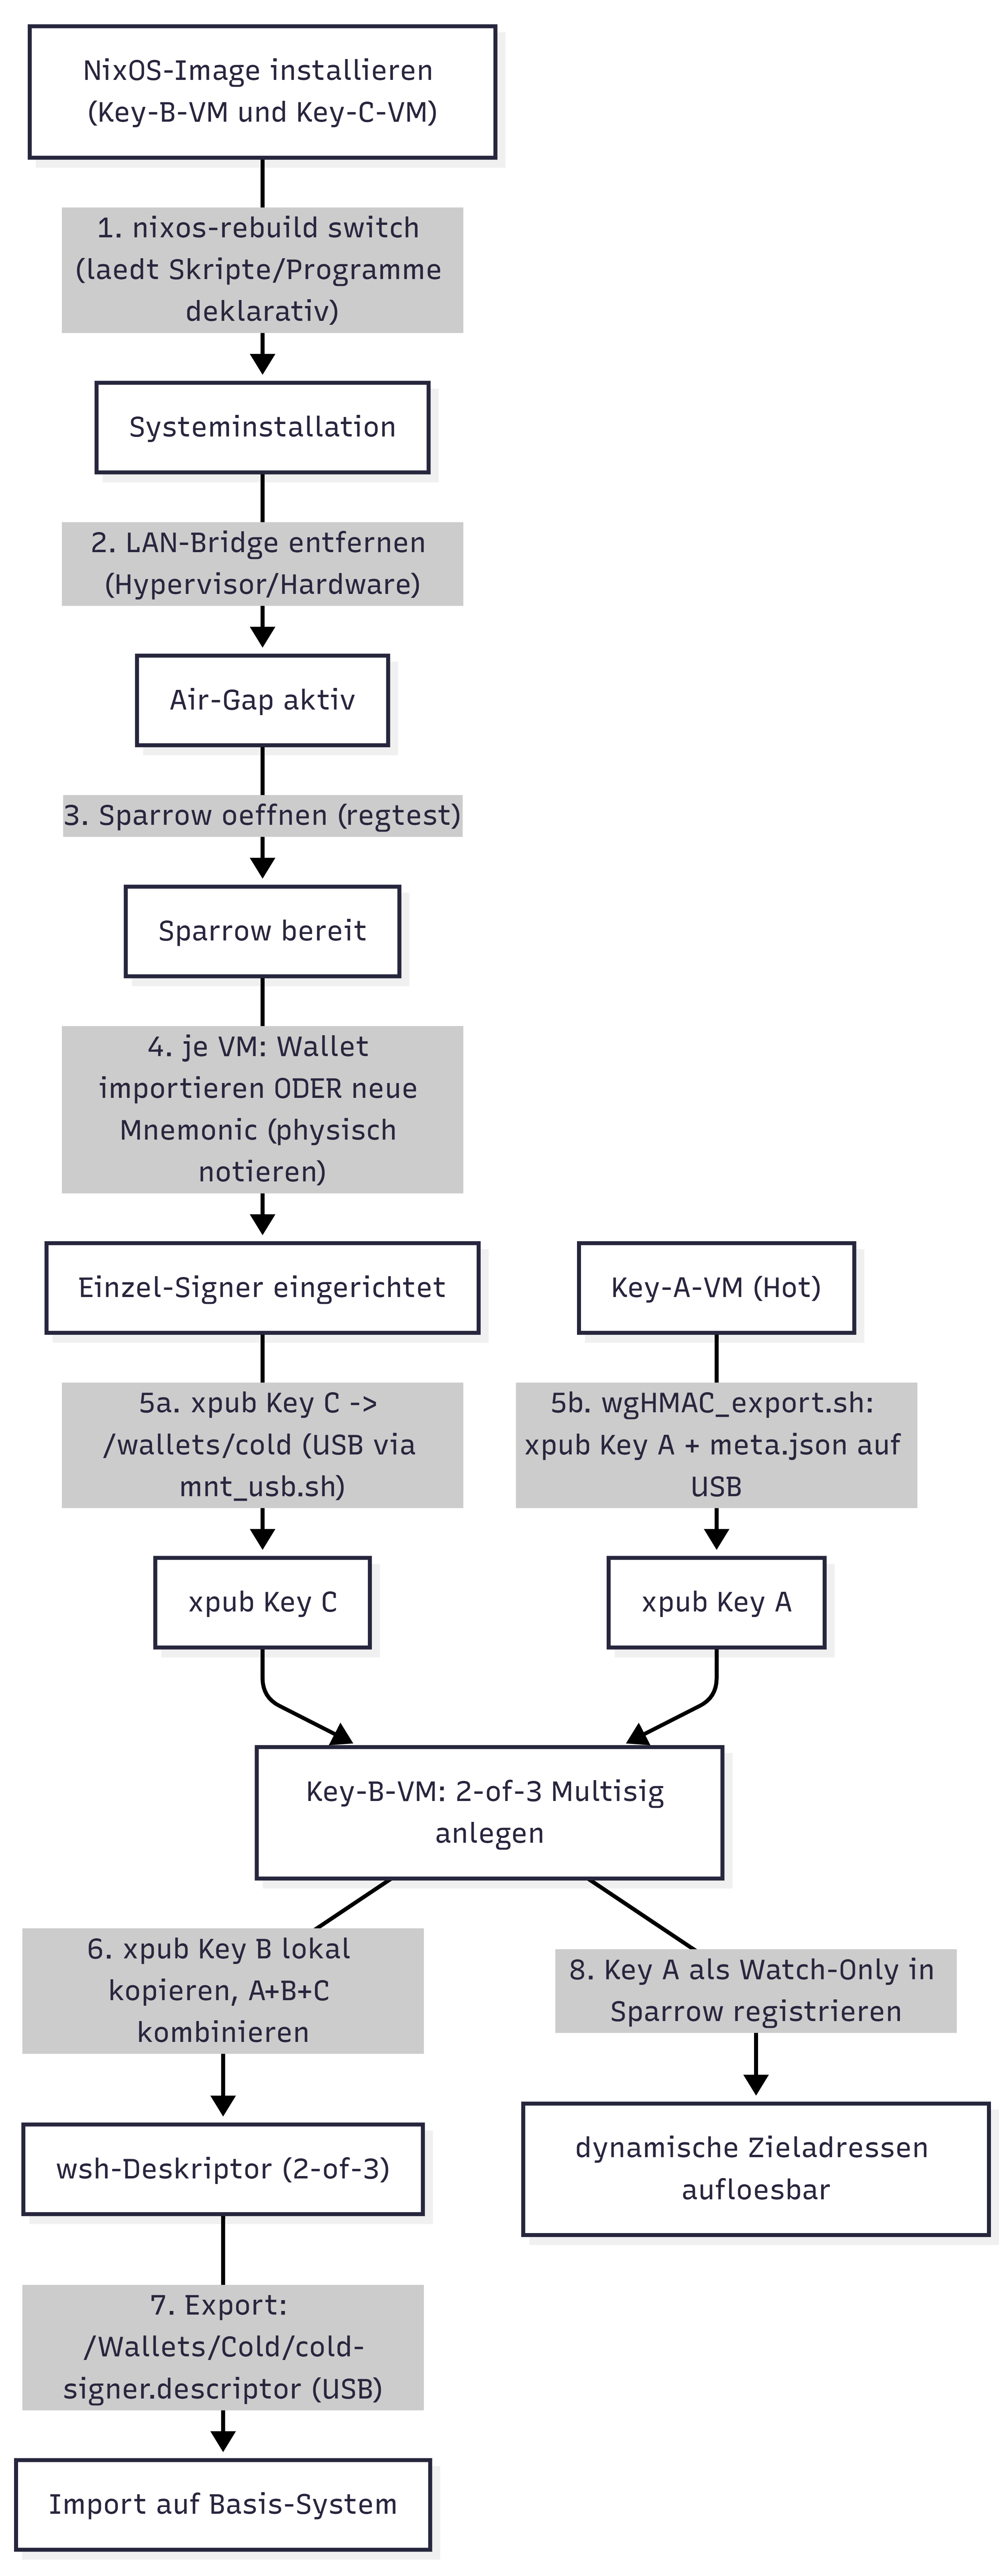
\includegraphics[width=0.55\textwidth]{Doku/Abbildungen/Cold-setup.png}
    \caption{Darstellung der Schritte zum Setup des Cold-Wallets. \\Quelle: Eigene Darstellung.}
    \label{fig4:cold_setup}
\end{figure}

Um den in Abbildung \ref{fig4:cold_setup} dargestellten Prozess zu vereinfachen, stehen auf den Cold- und Hot-Wallet-\acp{VM} Hilfsskripte zum Mounten, sicheren Auswerfen und Formatieren eines USB-Mediums auf dem Desktop bereit.

\subsubsection{Hot-Transaktionsprozess} \label{sec:hot_flow}

Der automatisierte Hot-Prozess verläuft entlang der zuvor beschriebenen Services (siehe Abbildung~\ref{fig7:psbt_hot}). 
Dabei nimmt die Middleware den Intent über eine der externen Schnittstellen entgegen (siehe
Tabelle~\ref{tab:tx_rails}), gleicht die Zieladresse gegen die Whitelist ab und beauftragt den TX-Builder über \ac{NATS} mit dem Bau der \ac{PSBT}.
Die fertige \ac{PSBT} wird anschließend durch \ac{OPA} autorisiert (siehe \ref{sec:opa}).

\begin{figure}[htbp]
    \centering
    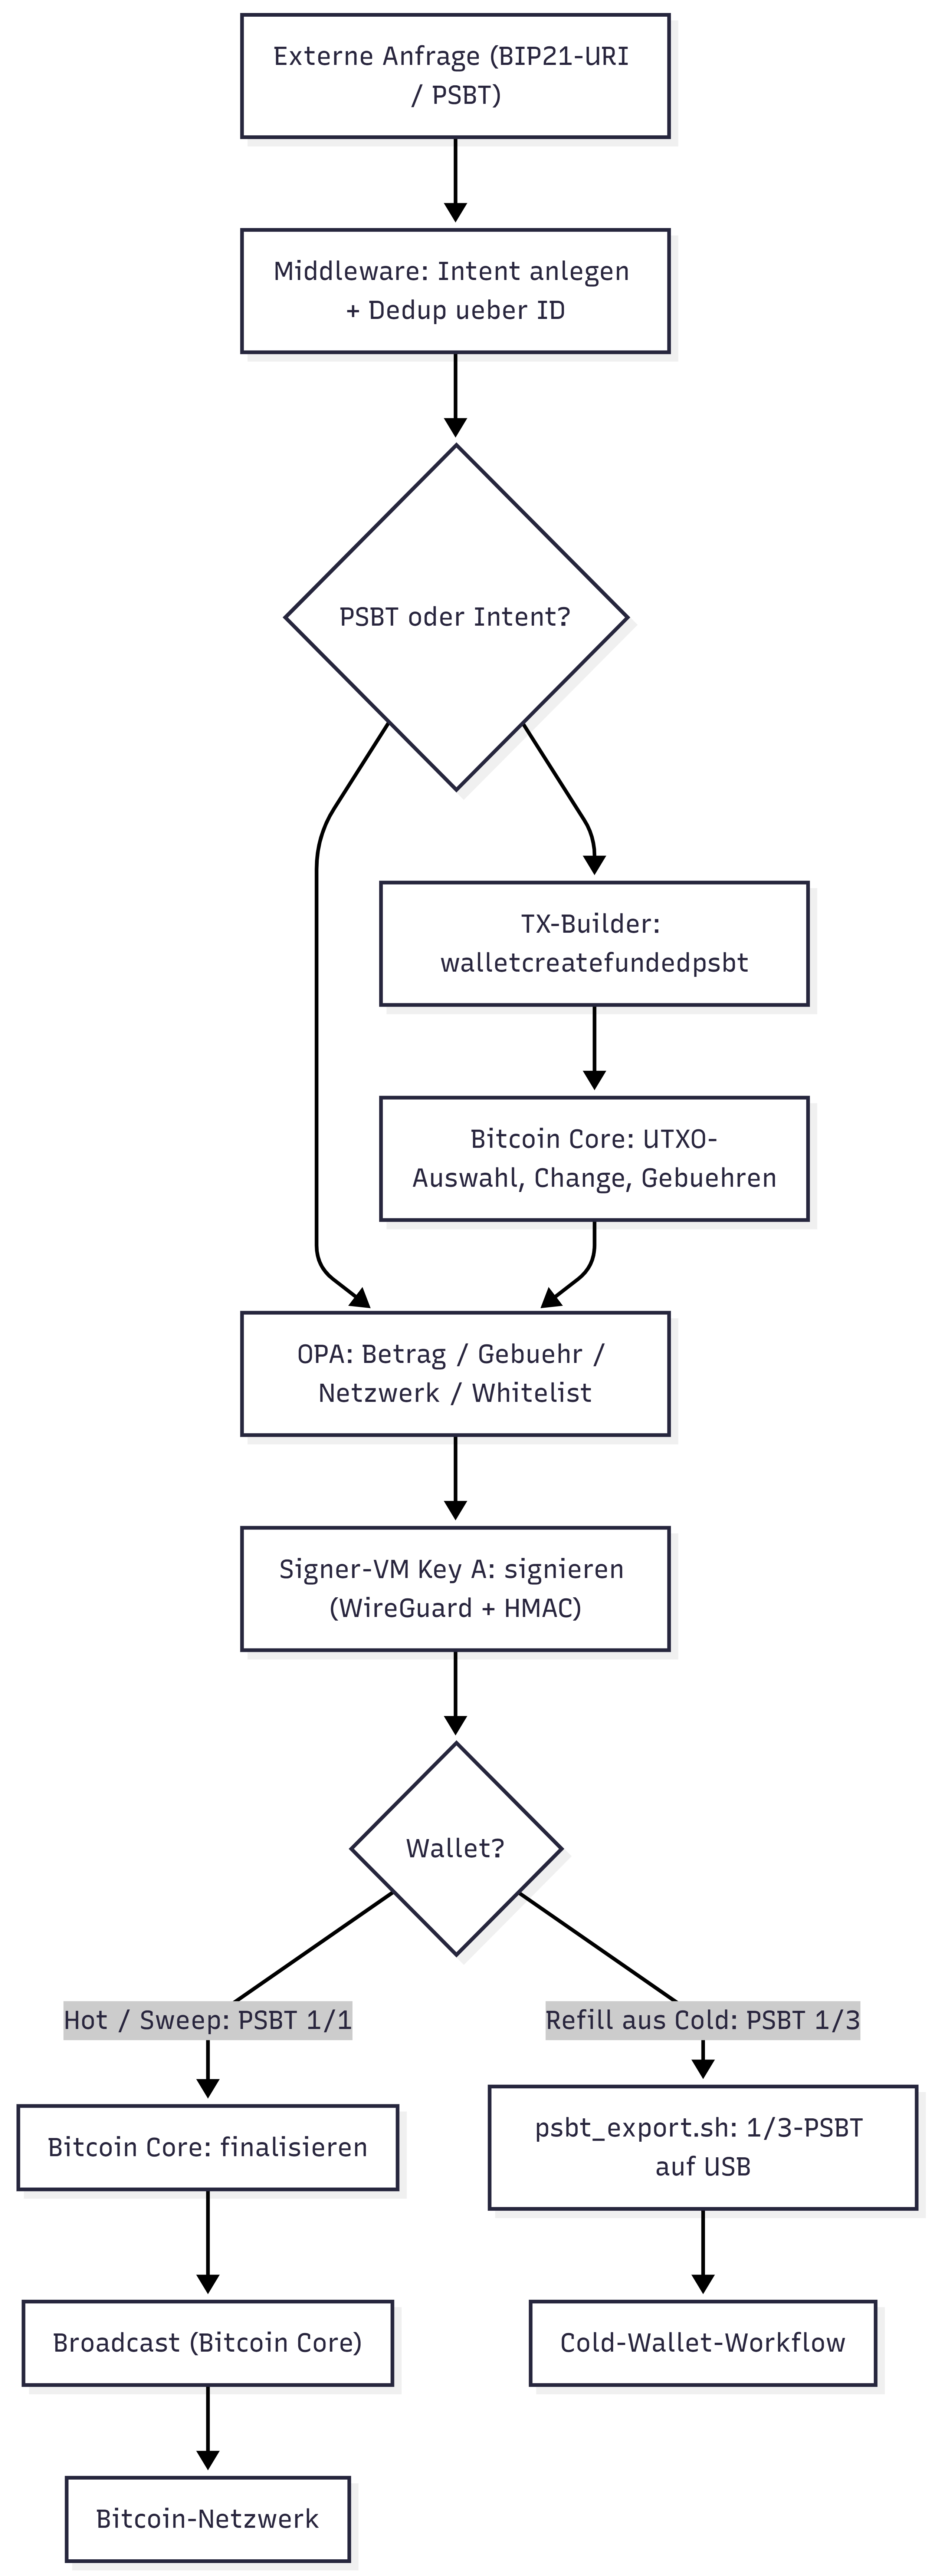
\includegraphics[width=0.7\textwidth]{Doku/Abbildungen/PSBT-Hot_workflow.png}
    \caption{Darstellung des Signierprozesses für das Hot-Wallet. \\Quelle: Eigene Darstellung.}
    \label{fig7:psbt_hot}
\end{figure}

Anschließend muss die \ac{PSBT} von Schlüssel~A signiert werden und wird dazu an die Signer-\ac{VM} übertragen. Von der Schlüssel-Halter-\ac{VM} wird eine \ac{PSBT} zurückgegeben. Im Falle des Cold-Wallets ist 1 von 3 Signaturen gegeben, und der Prozess muss asynchron durch den Mandanten fortgesetzt werden. Eine \ac{PSBT} des Hot-Wallets kann direkt über Bitcoin Core in eine finalisierte \ac{TX} umgewandelt und anschließend gebroadcastet werden.

Nach jedem Broadcast des Hot-Wallets wird über Bitcoin Core der Kontostand der Wallet über \path{getbalances()} abgefragt und anschließend wieder an \ac{OPA} weitergeleitet. Dieser bestimmt die Aktion, die Höhe der Transaktion und die \ac{PSBT}-Parameter. Anschließend wird die \ac{PSBT} wie im normalen Prozess gebaut und durch Key~A signiert. Im Fall einer Sicherungstransaktion vom Hot- zum Cold-Wallet wird sie am Ende automatisch gebroadcastet. Im Fall einer Nachfüllung von Cold zu Hot wird der Operator benachrichtigt, den manuellen Prozess des Signierens mit Key~B oder Key~C fortzuführen.

\subsubsection{Operator-Pfad}

Der als Rail \texttt{manual} bereits bei der Middleware eingeführte Operator-Pfad (siehe Tabelle~\ref{tab:tx_rails}) besitzt gegenüber den externen Rails zwei bewusste Ausnahmen.
Zum einen entfällt der Abgleich der Zieladresse gegen die externe Whitelist, sodass der Operator auch an nicht registrierte Adressen überweisen kann. Zum anderen überspringt \ac{OPA} für diesen Rail die Betrags- und Gebührengrenzen. Beide Ausnahmen sind erforderlich, damit der Operator im Ausnahmefall handlungsfähig bleibt. 
Als Restschranken bleiben der Besitz der Operator-\ac{NATS}-Zugangsdaten, die Pflichtfeld- und Struktur-Prüfung samt SHA-256-Nachweis in \ac{OPA}, der Tages-Cap (\texttt{\seqsplit{max\_daily\_sats}}, siehe \ref{sec:OPA_vel}) sowie als harter, unabhängiger Backstop der Velocity-Cap des Signers (siehe \ref{sec:keyA_vel}) bestehen. Der manuelle Pfad ist damit ein kontrollierter Bypass mit verbleibenden Schranken, kein ungeprüfter Kanal.

\subsubsection{Signierungs-Prozess} \label{sec:sparrow_signierung}

Der Cold-Wallet-Prozess startet für den menschlichen Operator mit der Benachrichtigung auf seinem GrapheneOS-Handy (zugestellt über den selbst gehosteten ntfy-Dienst, siehe \ref{sec:apphost-monitoring}). Zuvor wurde eine vordefinierte untere Grenze für den Stand der Geldmittel des Hot-Wallets unterschritten. Dadurch werden mehr Geldmittel benötigt, um die Operationalität des automatischen Systems zu gewährleisten. Die \ac{PSBT} für diese Transaktion wird vollautomatisch gebildet und signiert, sodass der Operator sie im nächsten Schritt auf dem Basis-System durch ein automatisches Skript, \path{psbt_export.sh}, in das Datei-System des Basis-System schreiben kann. Daraufhin muss diese Datei per \ac{SSH} vom Apphost auf den \ac{PC} des Operator und anschließend auf ein angeschlossenes \ac{USB}-Medium transferiert werden (siehe~\ref{sec:SSH}).
Das GrapheneOS-Handy des Operators wird nur zur Benachrichtigung von sicherheitskritischen Geschehnissen verwendet. Zu keinem Zeitpunkt befindet sich in unserem definierten Prozess geheimes Schlüsselmaterial darauf. Koordinatoren, die Software-Schlüssel auf einem Smartphone ablegen (etwa Nunchuks mobile App, siehe \ref{sec:alt_sparrow}), wurden aufgrund des fehlenden air-gap als Schlüsselhalter verworfen.

\begin{figure}[htbp]
    \centering
    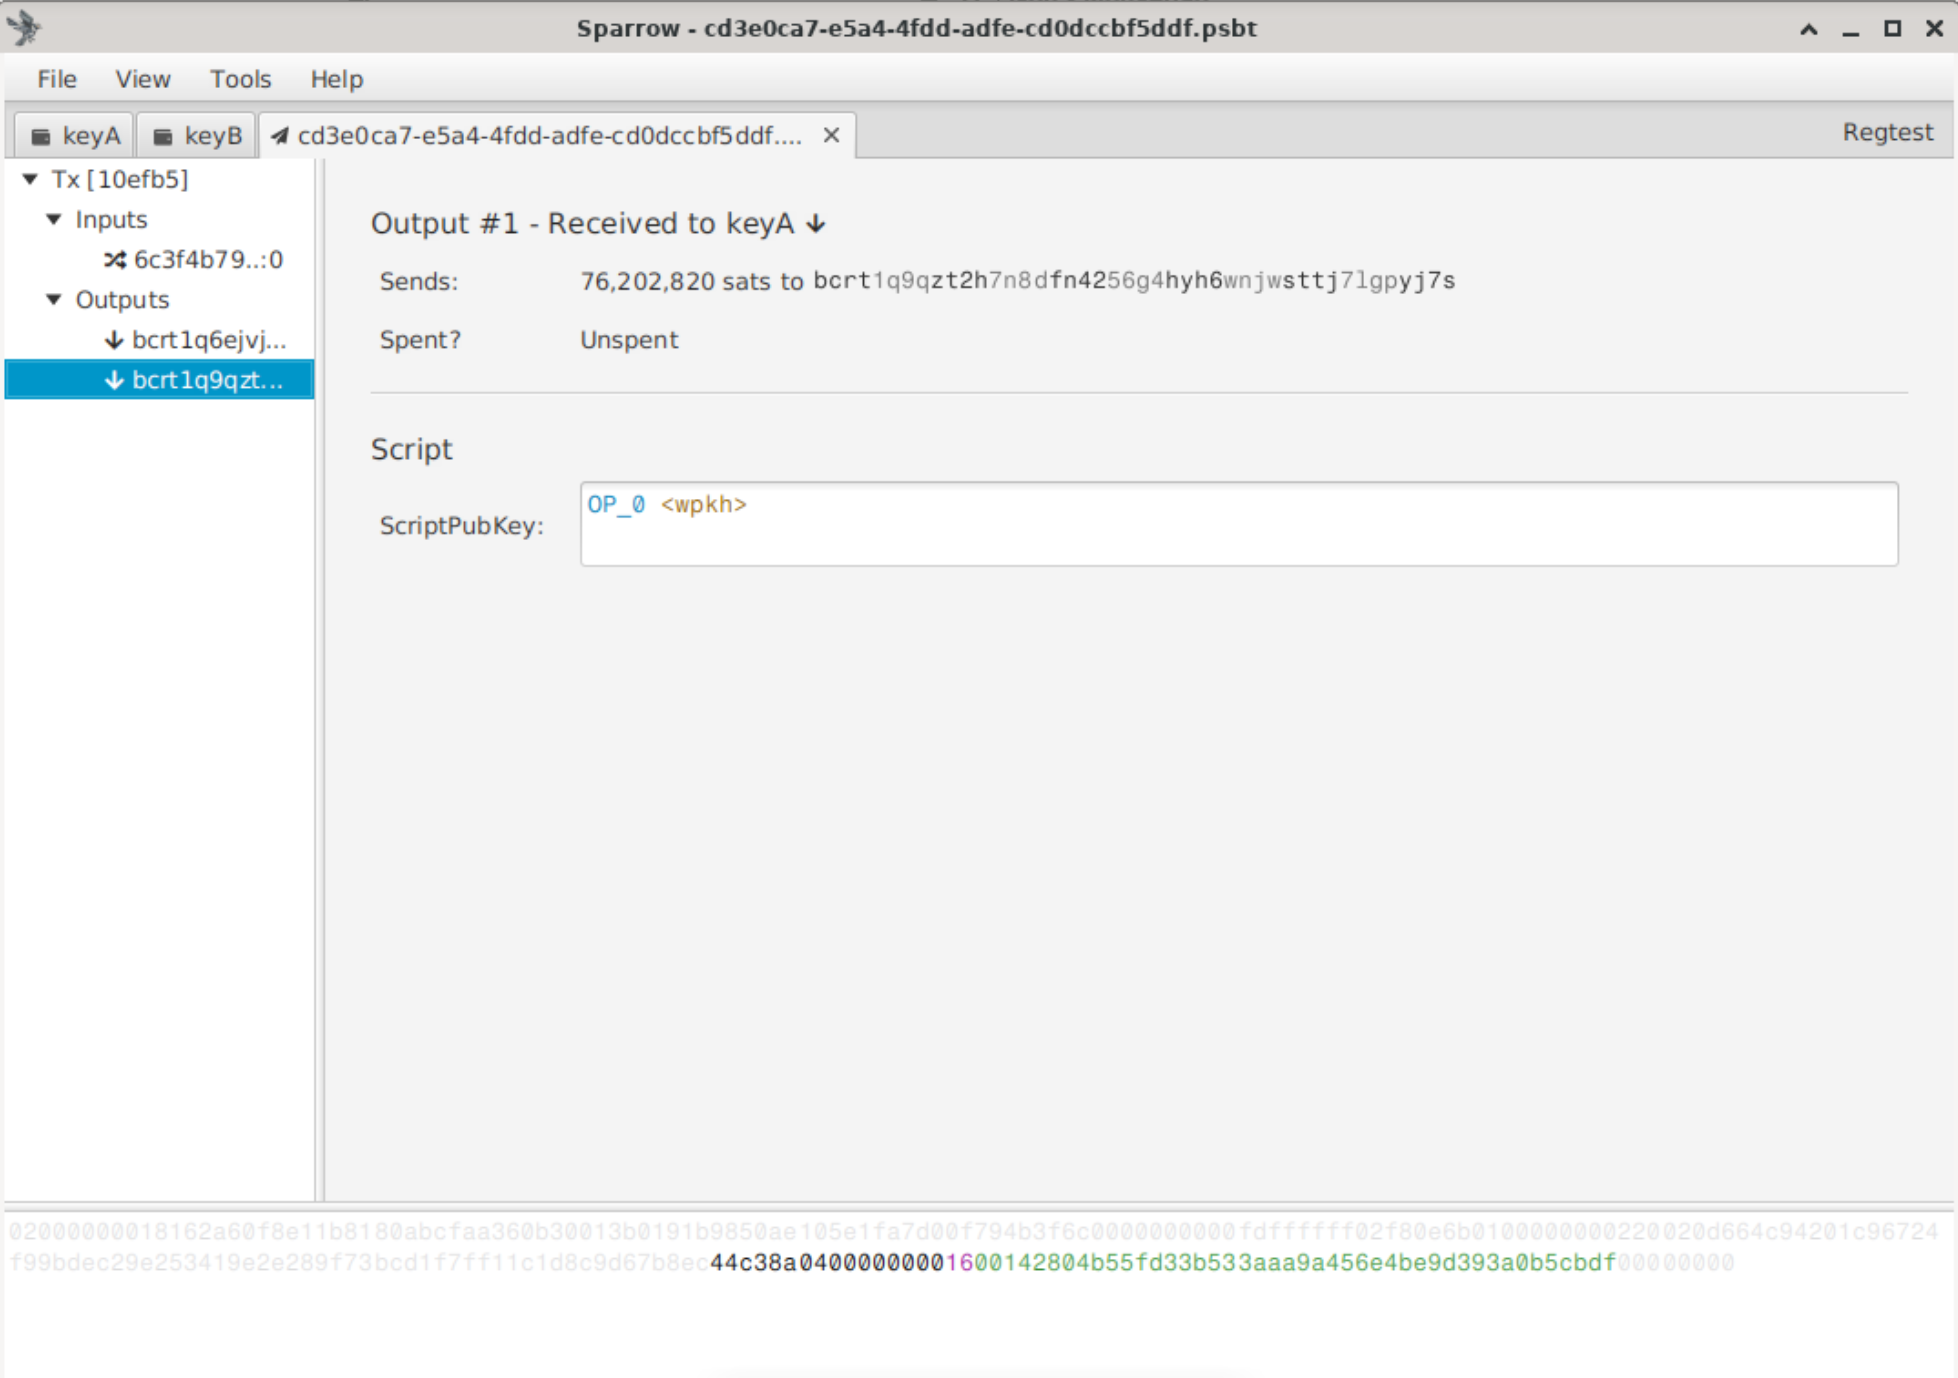
\includegraphics[width=0.8\textwidth]{Doku/Abbildungen/sparrow/sparrow_send_keyA.png}
    \caption{Darstellung der Sparrow Output-Verifikation. \\Quelle: Eigenes Bildschirm-Foto aus Sparrow.}
    \label{fig5:sparrow_output_verif}
\end{figure}

\label{sec:cold_sign}
Nach dem Umstecken auf die Key~B \ac{VM} muss der Operator die \ac{PSBT} in das Key~B Wallet importieren, die Details verifizieren und die \ac{PSBT} signieren.
Diese Verifizierung stellt sich wie im weiteren Verlauf in \ref{sec:alt_hash} kurz angesprochen als letzte Verteidigungsmaßnahme für das Cold-Wallet dar und stellt einen Grund für die Auswahl von Sparrow-Wallet unter den Alternativen dar (siehe \ref{sec:alt_sparrow}). Unter \path{Outputs} können die genauen Höhen der Bewegungsgrößen bestehend aus Coins, Übertragungswerten (\texttt{Output \#1}) und Wechselgeld (\texttt{Output \#0}) und deren Zieladressen angesehen werden. Durch das Hinzufügen des öffentlichen Key~A \ac{BIP}84 Single-Signatur Deskriptors als eigenständiges Wallet in Sparrow (siehe \ref{sec:sparrow_keyA_load}), wird die Zieladresse direkt als zu Key~A gehörig aufgelöst (siehe \texttt{\seqsplit{Output~ \#1~-~Received~to~KeyA}} in der Abbildung und bereits erwähnt in \ref{sec:dyn_adress}). Diese Visualisierung ist in Grafik \ref{fig5:sparrow_output_verif} dargestellt. Diskrepanzen in dieser Überprüfung führen dazu, dass die \ac{PSBT} nicht signiert werden darf und weisen auf eine Kompromittierung des Basis-Systems hin.

Nach der Signierung kann eine finalisierte \ac{TX} direkt als Datei mit der neuen Endung \path{.txn} auf dem Wechselmedium gespeichert werden. Dies ist wie in Abbildung \ref{fig6:sparrow_broadcast} direkt über den Knopf \texttt{Save Final Transaction} auf Sparrow möglich. Das dargestellte Bild zeigt zudem das als Alternative beschriebene direkte Broadcasting über Sparrow im Online-Modus aus Kapitel \ref{sec:alt_Sparrow_broadcast}.
Danach kann das \ac{USB}-Medium wieder in den \ac{PC} des Mandanten eingesteckt, die Datei per \ac{SSH} in den Apphost transferiert werden und über das Skript \path{psbt_broadcast.sh} importiert sowie automatisch über Bitcoin Core gebroadcastet werden (siehe~\ref{sec:SSH}).

\begin{figure}[htbp]
    \centering
    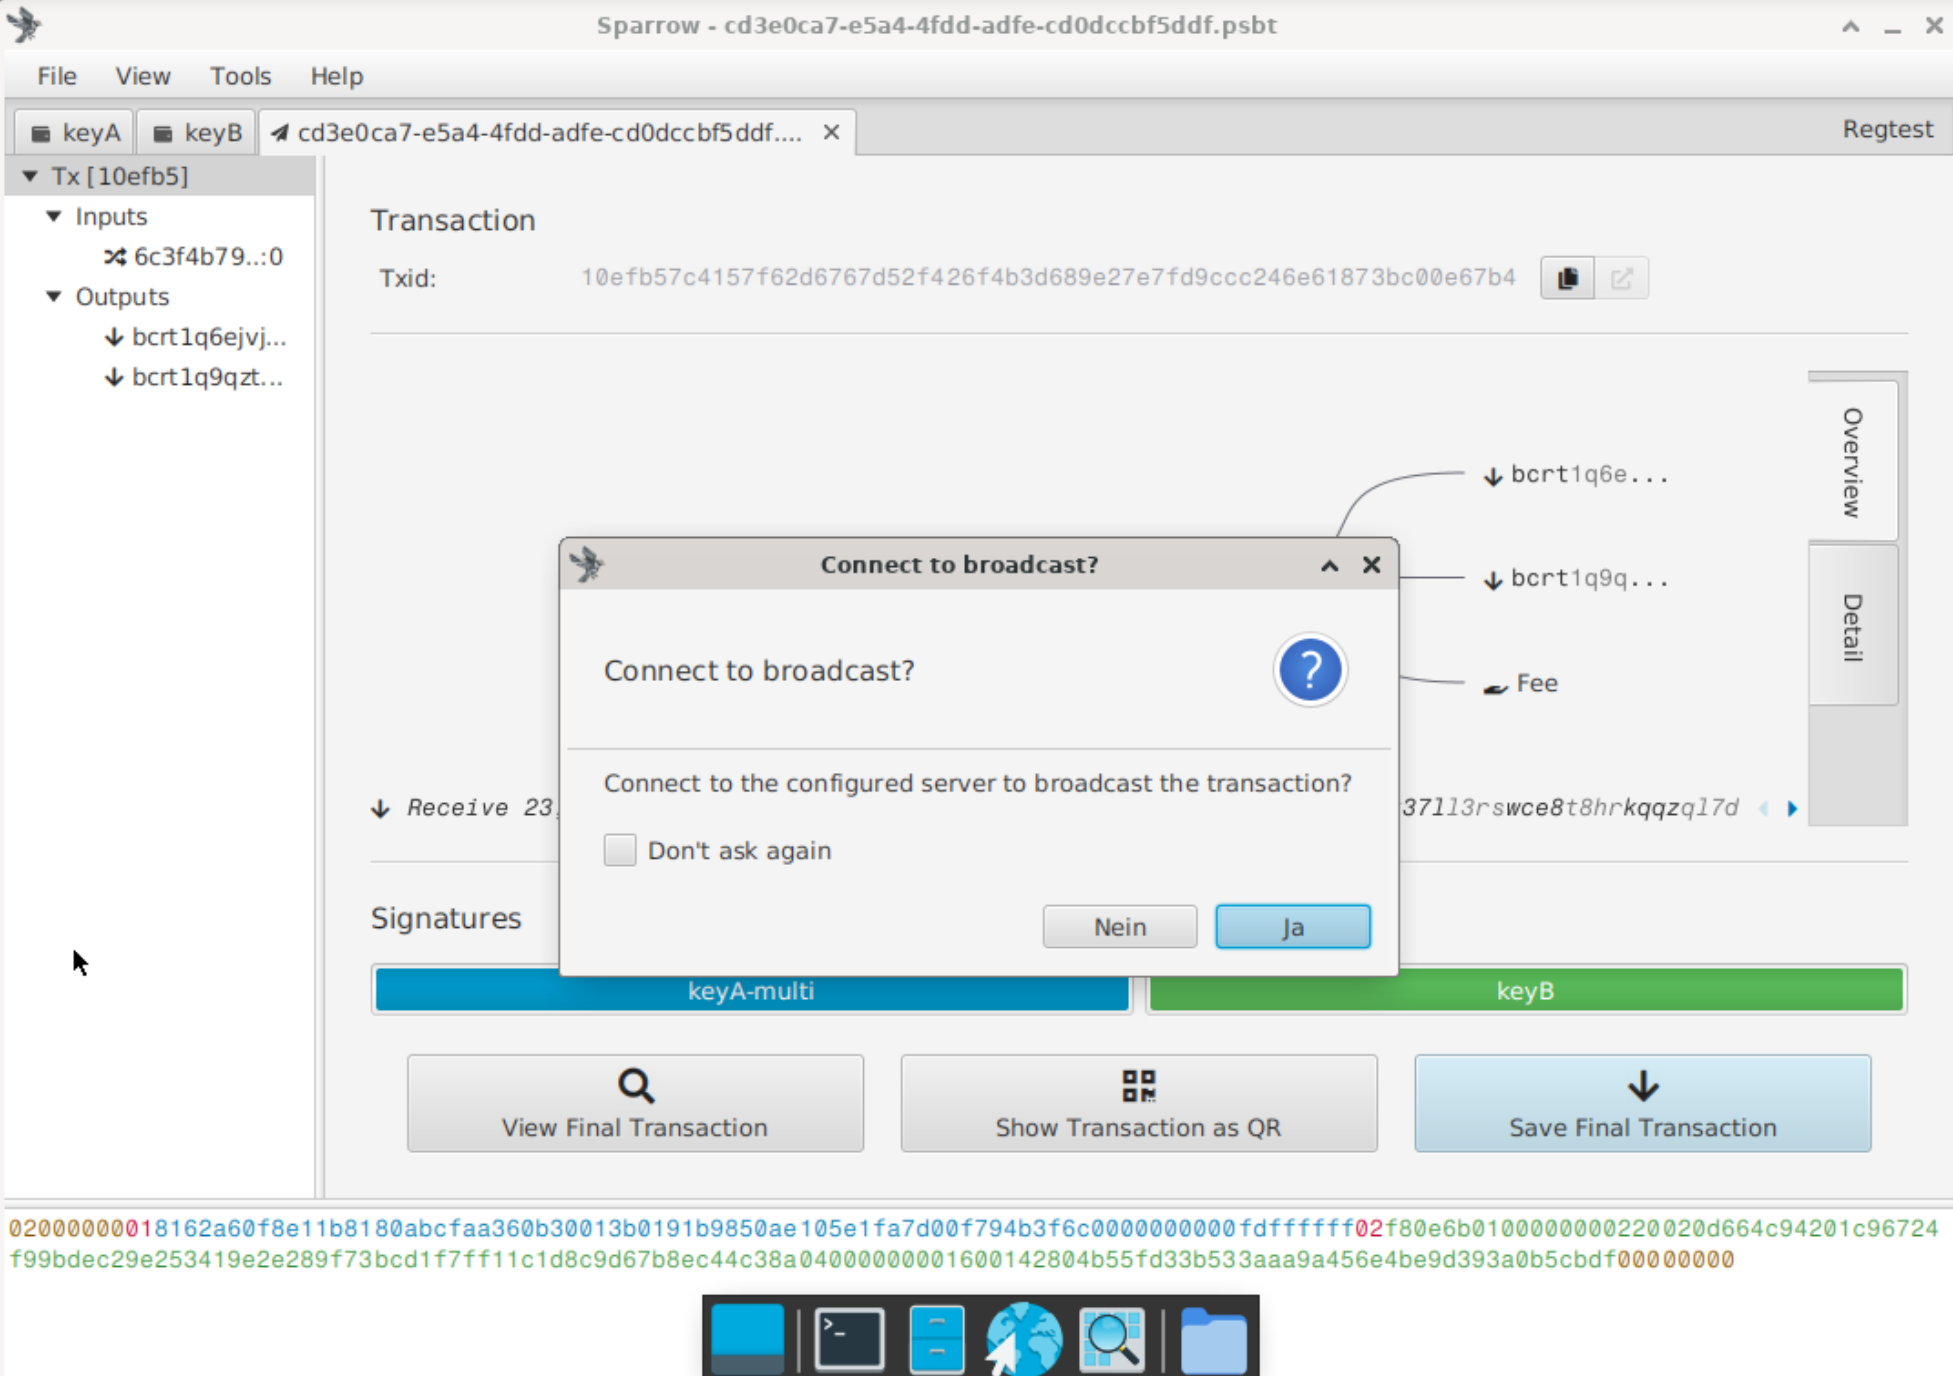
\includegraphics[width=0.8\textwidth]{Doku/Abbildungen/sparrow/sparrow_broadcast.png}
    \caption{Sparrow Wallet Broadcast und Final \ac{TX} Export Funktion nach Signatur. \\Quelle: Eigenes Bildschirm-Foto aus Sparrow.}
    \label{fig6:sparrow_broadcast}
\end{figure}

Eine tiefere Beschreibung der Konfiguration und des gesamten Setup- und Signierungsprozesses kann in der \path{README.md} des NixOsCold-GitHub nachgelesen werden \cite{NixOsCold_github}. Eine Kurzübersicht aller Skripte bietet Tabelle~\ref{tab:skripte} im Anhang.

\begin{figure}[htbp]
    \centering
    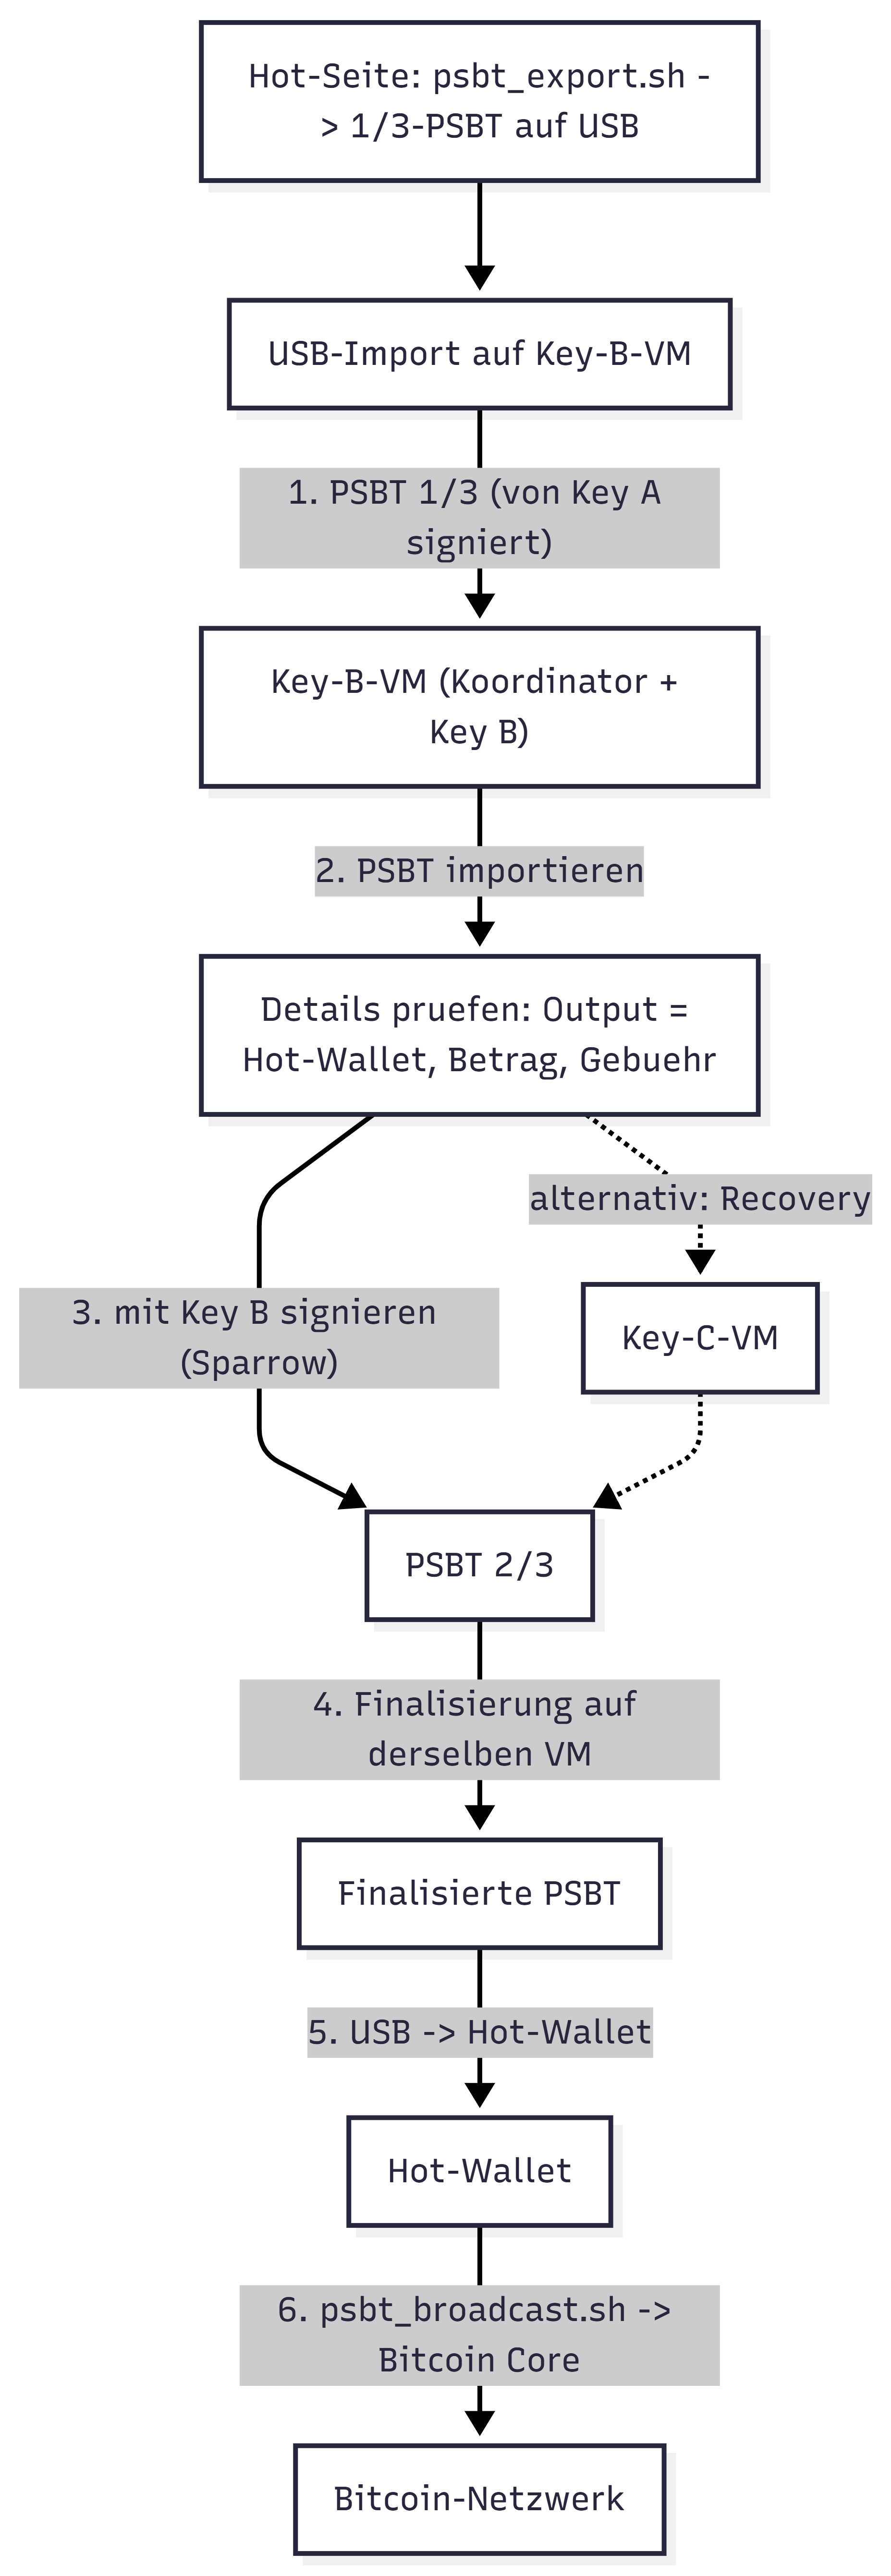
\includegraphics[width=0.5\textwidth]{Doku/Abbildungen/PSBT-Cold_Workflow.png}
    \caption{Darstellung des Signierprozesses für das Cold-Wallet. \\Quelle: Eigene Darstellung.}
    \label{fig6:cold_signing}
\end{figure}

\subsubsection{Refill-Lebenszyklus}

Da bis zur Befüllung durch den asynchronen Cold-Prozess geraume Zeit vergehen kann, müssen die Balance-Grenzen der \texttt{hot.limits}-Policy (siehe \ref{sec:opa}) mit ausreichend Puffer gewählt werden.
Diese wurden, wie beschrieben, als weitere \ac{OPA}-Policy umgesetzt und können in der \path{data.json} durch den Mandanten an seine Geldmittel angepasst werden.
Da der automatisierte Hot-Flow während der Wartezeit des asynchronen Cold-Prozesses unverändert weiterläuft und nach jedem Broadcast erneut eine Balance-Prüfung über die \texttt{hot.limits}-Policy auslöst, kann der Nachbefüllungsbedarf in dieser Phase mehrfach gemeldet werden. Ohne Gegenmaßnahme entstünden dadurch konkurrierende Nachbefüllungs-\acp{PSBT} für unterschiedliche Höhen desselben Mangels, und der Operator könnte veraltete \acp{TX} signieren.
Zudem kann deren Broadcast zu einer Überbefüllung des Hot-Wallets und damit zu einem gegenläufigen \texttt{hot\_to\_cold}-Intent führen, wodurch Zeit des Operators und Gebühren für die eiligen Transaktionen verschwendet würden.

Zur Auflösung der Problematik wurde sich für eine Logik entschieden, bei der sich zu jedem Zeitpunkt nur genau eine aktive Nachbefüllungs-\ac{PSBT} im System befindet. Die persistente Ablage hält stets nur die jeweils jüngste Nachbefüllungs-\ac{PSBT} vor. Eine neu erzeugte \ac{PSBT} ersetzt eine bereits wartende durch Überschreiben der Datei.

Zudem wird der Lebenszyklus über drei gezielte Löschpunkte abgesichert:
Beim Export auf das Wechselmedium wird die wartende \ac{PSBT} eingelesen, aus der persistenten Ablage entfernt und in den Zustand \linebreak COLD\_STARTED überführt. Ab diesem Punkt gilt die Transaktion als in der Hand des Operators. Die Single-\ac{TX}-Prüfung des Export-Skripts verhindert, dass eine weitere \ac{PSBT} auf dasselbe Medium gelangt. Die persistente Ablage der Datei wird gelöscht, sodass der Signierungsprozess nicht erneut gestartet werden kann und damit die \ac{PSBT}-Status-\ac{DB} als Source of Truth nicht gestört werden könnte.

Beim Broadcast der signierten Cold-\ac{PSBT} wird erneut eine Löschung ausgelöst. Diese greift gezielt den Fall ab, dass während der Wartezeit des Operators, also zwischen Export und Broadcast, eine weitere Nachbefüllungs-\ac{PSBT} erzeugt und in der Ablage hinterlegt wurde. Da der soeben abgeschlossene Broadcast den ursprünglichen Mangel in einer gewissen Höhe bereits behoben hat, wäre eine solche zwischenzeitlich entstandene \ac{PSBT} auf einen überholten Saldo gestützt und wird daher verworfen.

Der dritte Löschpunkt besteht in der vollautomatischen Löschung der Nachbefüllungs-\ac{PSBT}, wenn diese noch nicht vom Operator aufgenommen wurde. Die Löschung wird ausgelöst, wenn \ac{OPA} eine \texttt{hot\_to\_cold}- oder \texttt{hold}-Aktion ermittelt. Dementsprechend muss seit Generierung der \ac{PSBT} dem Hot-Wallet eine ausgleichende Menge an Geldmitteln gutgeschrieben worden sein, was erst mit der nächsten Hot-\ac{TX} auffällt.
Praktisch stammt dieser Zufluss, der den Hot-Saldo wachsen lässt, aus regulären eingehenden Zahlungen Dritter an das Hot-Wallet. \texttt{hot\_to\_cold} und \texttt{cold\_to\_hot} Zahlungen wurden bereits von den anderen Löschpunkten abgedeckt.
Solche \acp{TX} können von jedem Wallet-Inhaber ohne Zustimmung der Zieladresse ausgeführt werden wie wir es ebenfalls vornehmen. Da es sich bei dem Hot-Wallet um ein vollautomatisches \ac{TX}-System handelt, ist der Fall, dass Partner ebenfalls Geld auf dieses Wallet senden, denkbar und musste in die Logik eingeplant werden.

Ein verbleibender Randfall besteht, wenn der ausgleichende Zufluss erfolgt, nachdem die Nachfüll-\ac{PSBT} erzeugt, aber bevor eine weitere Hot-Transaktion die Balance-Prüfung erneut auslöst. Nimmt der Operator die zu diesem Zeitpunkt bereits obsolete \ac{PSBT} auf, ist sie nach dem Export keinem der drei Löschpunkte mehr zugänglich. Ihr Broadcast führt dann zu einer Überbefüllung und einer gegenläufigen \texttt{hot\_to\_cold}-Transaktion mit doppeltem Gebührenanfall. Eine vollständige Absicherung wäre durch eine erneute Bedarfsprüfung unmittelbar vor dem Broadcast erreichbar, wobei ein \ac{ZMQ}-basiertes Mithören auf Zuflüsse, das bei einer \ac{TX}-Erkennung für das Hot-Wallet eine Reevaluierung durch \ac{OPA} auslöst, das Fenster zwar verkleinern, aber aufgrund des verbleibenden Export-Zeitpunkts nicht schließen würde. Aufgrund der geringen Eintrittswahrscheinlichkeit wurde der Randfall als akzeptabel eingestuft.

Ein aktiver Neuaufbau der Nachfüll-\ac{PSBT} nach der Löschung erfolgt anschließend nicht. Stattdessen bleibt die Ablage leer, bis die nächste reguläre Hot-Transaktion über die Balance-Prüfung erneut einen Bedarf feststellt. Dadurch basiert jede neu erzeugte Nachbefüllungs-\ac{PSBT} zwangsläufig auf dem aktuellen, nach dem letzten Broadcast gültigen Wallet-Stand, womit zugleich das Problem einer auf veraltetem Saldo beruhenden Empfehlung strukturell ausgeschlossen ist.

Für eine einfachere Bedienung durch den Operator können folgende Skripte im Basis-System ausgeführt werden:
\begin{itemize}
    \item \path{/ops/refill/psbt_export.sh}: exportiert die letzte Cold-\ac{PSBT} auf ein Wechselmedium unter \path{/psbt/<id>.psbt} und erfüllt die Voraussetzung für den Cold-Signierungsprozess.
    \item \path{/ops/refill/psbt_broadcast.sh}: importiert eine Cold-\ac{PSBT} von einem Wechselmedium aus \path{/psbt/<id>.txn}.
\end{itemize}

Zudem wird mit \path{/ops/refill/psbt_broadcast.sh} die \ac{PSBT} an das Basis-System weitergegeben, die \ac{PSBT}-Details wie \ac{ID}, \ac{SATS}-Menge und Adresse mit der \ac{DB} abgeglichen und diese nach Bestätigung finalisiert und gebroadcastet.

\subsubsection{Produktivübernahme - Mainnet-Migration} \label{sec:mainnet_migration}
Die Laborumgebung ist durchgängig auf das Regtest-Netzwerk ausgelegt. Bei der Übernahme in den Produktivbetrieb genügt es nicht, lediglich den Netzwerkmodus umzustellen, da sich mit dem Netzwerk auch der Coin-Type der \ac{BIP}32-Ableitungspfade ändert (Testnet/Regtest: \path{1'}, Mainnet: \path{0'}). 
Aus \path{m/84'/1'/0'} wird \path{m/84'/0'/0'} und aus \path{m/48'/1'/0'/2'} wird \path{m/48'/0'/0'/2'}. Damit sind sämtliche \acp{xpub}, Deskriptoren und die daraus registrierten Wallets neu zu erzeugen und erneut über das Wechselmedium auszutauschen. Für die Migration sind
folgende Schritte erforderlich:
\begin{itemize}
    \item Umstellung von Bitcoin Core auf das Mainnet und initiale
          Blockchain-Synchronisation,
    \item Umstellung des Sparrow-Netzwerkmodus auf allen Schlüsselhalter-\acp{VM},
    \item Neuerzeugung der Seeds beziehungsweise Neuableitung der Mainnet-Pfade,
          Neuaufbau des Multi-Signatur-Wallets (siehe \ref{sec:cold_setup}) und
          erneuter Deskriptor-Import auf dem Basis-System,
    \item Anpassung der \ac{OPA}-Regel \texttt{Netzwerk} in \path{data/data.json},
          die im Auslieferungszustand ausschließlich \texttt{regtest} zulässt
          (siehe Tabelle~\ref{tab:opa_hot}).
\end{itemize}

\subsection{Alternativen} \label{sec:alt_alg}
Neben der primär dargestellten Implementation kann der Mandant nach Übergabe des simulierten Systems entscheiden, zu anderen Ansätzen zu wechseln. Wie bei den Sparrow-Wallet Alternativen in \ref{sec:alt_sparrow} wurden verschiedene Ansätze evaluiert und werden in diesem Abschnitt diskutiert.

\subsubsection{Hardware-Wallets}
Es bietet sich an, dedizierte Hardware-Wallets anstelle der Key-Holder-NixOS-\acp{VM} zu verwenden. Diese haben sich als etablierter Industriestandard für die Verwahrung von Bitcoin-Schlüsselmaterial
herausgebildet. Verbreitete Geräte sind dabei quelloffen oder zumindest mit einsehbarer Firmware verfügbar. Ihr wesentlicher Sicherheitsgewinn liegt in einem dedizierten Display auf der Gerätehardware, über das \ac{TX}-Details unabhängig vom angeschlossenen Rechner verifiziert werden können. Dies ist analog zu der in unserem Prozess vorgesehenen manuellen Verifikation in Sparrow Wallet,
jedoch auf einer eigenständigen, sehr schwer kompromittierbaren Hardware.

\subsubsection{Electrum-Server} \label{sec:electrum_serv}
Ein Electrum-Server wie \texttt{ElectrumX}, \texttt{electrs} oder \texttt{Fulcrum} ist eine Server-Software, die zwischen einer Bitcoin-Full-Node und leichtgewichtigen Wallet-Clients vermittelt. Er indexiert die Blockchain nach Adressen bzw.\ Script-Pubkeys, sodass eine Wallet über das Electrum-Protokoll effizient die \acp{UTXO} und die Transaktionshistorie ihrer Adressen abfragen kann, ohne selbst die gesamte Kette durchsuchen zu müssen. Sowohl Electrum als auch Sparrow lassen sich auf diese Weise anbinden.

Bei Nutzung eines \emph{öffentlichen} Electrum-Servers übermittelt die Wallet dem Serverbetreiber sämtliche zugehörigen Adressen, wodurch dieser erkennt, welche Adressen zu derselben Wallet gehören. Über die öffentliche Blockchain kann der Betreiber zudem deren Guthaben, Aktivität und Metadaten ermitteln und mit der IP-Adresse verknüpfen. Es besteht zwar keine Gefährdung der Assets, da beim Broadcast nur die fertig signierte, öffentliche Transaktion übertragen wird und kein privates Schlüsselmaterial, jedoch ein Verlust an Privatsphäre gegenüber Dritten.

Im vorliegenden System entfällt ein Electrum-Server vollständig, da das Hot-System bereits einen eigenen Bitcoin-Core-Full-Node betreibt. Sämtliche Adress- und \ac{UTXO}-Abfragen zur Generierung der \acp{PSBT} verbleiben damit auf der selbst gehosteten Infrastruktur, ohne Offenlegung gegenüber Dritten. 
Die air-gapped Cold-\acp{VM} benötigen ohnehin keinen Server, da sie die Transaktionsdetails ausschließlich aus der \ac{PSBT} selbst verifizieren. Die Möglichkeit, Sparrow für einen alternativen Broadcast-Schritt direkt an Bitcoin Core anzubinden, bleibt dem Mandanten offen (siehe \ref{sec:alt_Sparrow_broadcast}).
Der Betrieb eines \emph{selbst gehosteten} Electrum-Servers kann Adressabfragen bei Wallets mit umfangreicher Historie beschleunigen, bringt für die hier verwendeten, frisch erzeugten Watch-Only-Wallets jedoch keinen relevanten Vorteil und verbleibt im Ermessen des Mandanten \cite{sparrow_quick,Sparrow_Wallets_Node_Connect, electrumx_docs}.

\subsubsection{Datentransfer}
Der Mandant kann den \ac{USB}-Austausch ebenfalls durch die Generierung von \ac{QR}-Codes und eine Kamera an den \acp{VM} oder durch direkte Hardware-Wallets ersetzen. Dies sollte die Möglichkeit einer Manipulation in Transit weitestgehend unterbinden, wobei die Transaktionsdetails weiterhin kontrolliert werden sollten \cite{Wallets,knowingbitcoin_airgap,Hardware_VS_Cold-Wallet}. Eine nötige Verbindung zum Apphost per \ac{SSH} bleibt bestehen.
Zudem konnten diese Übertragungstechnologien wie auch die Hardware-Wallets nicht in der Proxmox-Laborumgebung virtualisiert werden. Der implementierte \ac{USB}-Austausch stellt sich als einfaches Wechseln des Besitzers einer virtualisierten Festplatte dar und ließ sich somit sehr gut für die spätere praktische Verwendung simulieren.

\subsubsection{Online-Koordinator} \label{sec:alt_Sparrow_broadcast}
Ein früherer Architekturansatz sah vor, die Koordinator-Instanz nicht vollständig air-gapped zu betreiben, sondern diese über eine direkte Netzwerkverbindung an Bitcoin Core anzubinden.
Dieser Ansatz basiert auf der nativen Unterstützung von Sparrow Wallet, über eine direkte Verbindung mit einem Bitcoin-Core-Node zu kommunizieren. In diesem Szenario hätte Sparrow die vollständige Verarbeitungskette im Cold-Kontext übernehmen können:
\begin{itemize}
    \item Import und Verifikation der \ac{PSBT},
    \item Koordination und Durchführung der Multi-Signatur-Signierung,
    \item Finalisierung der Transaktion,
    \item direkter Broadcast an das Bitcoin-Netzwerk über die bestehende Node-Verbindung.
\end{itemize}

Die Funktionalität des direkten Broadcast nach der Signierung kann in Abbildung \ref{fig6:sparrow_broadcast} nachvollzogen werden.
Die Cold-Architektur hätte in diesem Fall aus drei getrennten Systemen bestanden:
\begin{itemize}
    \item Key~B (vollständig air-gapped),
    \item Key~C (vollständig air-gapped),
    \item Koordinator (netzwerkfähig, ohne Zugriff auf Schlüsselmaterial).
\end{itemize}

Durch die native Integration von Sparrow Wallet mit Bitcoin Core bietet sich dieser Ansatz technisch an, da keine zusätzliche Infrastruktur für den Broadcast erforderlich ist und der gesamte Transaktionsprozess innerhalb des Koordinators abgeschlossen werden kann.
Im weiteren Verlauf wurde dieser Ansatz jedoch verworfen, da er durch ein weiteres System mehr Last für den Operator bedeutet und zwei verschiedene Wege für das Broadcasting darstellt. Dies sollte konsolidiert und schlanker werden, wodurch sich sowohl die Angriffsfläche des Gesamtsystems als auch der Bedarf an Ressourcen verringert.

In einem zugehörigen früheren Ansatz wurde Sparrow Wallet im Cold-System direkt mit Bitcoin Core verbunden und das Cold-Wallet über diese Integration registriert. Diese Idee wurde verworfen, da sich für einen einheitlichen Import der Hot- und Cold-Wallet-Deskriptoren entschieden wurde und der Koordinator mit dem Schlüsselmaterial-Halter für Key~B zusammengelegt werden sollte. Dementsprechend sollte diese Maschine zu keinem Zeitpunkt nach dem Setup mit dem Internet verbunden sein, weshalb das Air-Gap direkt nach dem Build angewandt wird.

Insbesondere ergeben sich folgende Nachteile:
\begin{itemize}
    \item Der Cold-Bereich ist noch weiter vom Netzwerk abhängig, womit das ursprüngliche Sicherheitsmodell aufgeweicht wird,
    \item die Koordinator-Instanz wird zu einem aktiven Bestandteil der sicherheitskritischen Entscheidungslogik und muss zusätzlich vertraut werden,
    \item potenzielle Angriffe auf die Benutzerinteraktion oder die Anzeige der Transaktionsdetails können nicht mehr vollständig ausgeschlossen werden.
\end{itemize}

Die gewählte Architektur trennt hingegen klar zwischen Entscheidungs- und Kommunikationsdomäne:
\begin{itemize}
    \item Cold-Systeme übernehmen ausschließlich die Verifikation und Signierung,
    \item das Hot-System übernimmt den Broadcast.
\end{itemize}

Nichtsdestotrotz stellt diese Variante für bestimmte Anwendungsfälle eine valide Alternative dar.
Insbesondere bei reduziertem Fokus auf maximale Isolation oder erhöhten Anforderungen an die Bedienbarkeit kann die Integration des Broadcasts in die Koordinator-Instanz den operativen Aufwand deutlich reduzieren. Durch die Reduktion manueller Schritte, insbesondere des Rücktransfers der finalisierten Transaktion, kann die Fehleranfälligkeit im operativen Prozess gesenkt werden.

\subsubsection{Hashing} \label{sec:alt_hash}
Zusätzlich zur beschriebenen Multi-Signatur-Architektur wurde eine ergänzende, Hash-basierte Freigabeschicht evaluiert. Diese dient nicht der Autorisierung der Bitcoin-Transaktion selbst, sondern der Absicherung des organisatorischen Freigabeprozesses während des physisch getrennten Datentransfers.
Im Rahmen dieses Ansatzes wurde auf der Koordinator-Instanz ein separates kryptographisches Schlüsselpaar generiert. Der zugehörige Public Key wird über ein Wechselmedium auf die Signer-Systeme übertragen und dort hinterlegt.

Für jede freizugebende \ac{PSBT} wurde ein zusätzlicher Freigabemechanismus angewendet:
\begin{itemize}
    \item Erstellung eines kryptographischen Hashes der \ac{PSBT},
    \item Signierung dieses Hashes durch den Koordinator,
    \item Übertragung der Signatur zusammen mit der \ac{PSBT},
    \item Verifikation der Signatur auf den Key-Holder-Systemen.
\end{itemize}

Hierdurch kann überprüft werden, ob eine Transaktion tatsächlich durch die Koordinator-Instanz autorisiert wurde und während des Transports nicht verändert wurde.
Insbesondere in Szenarien mit erhöhten Anforderungen an Auditierbarkeit, mehreren Operatoren, langen Pausen oder bei stark regulierten Prozessen kann eine solche zusätzliche Verifikationsschicht sinnvoll sein. Ebenso kann sie in Umgebungen mit reduziertem Vertrauen in den manuellen Prozess zusätzliche Sicherheit bieten.

Im weiteren Verlauf der Ausarbeitung wurde dieser Mechanismus nicht als Bestandteil der finalen Architektur übernommen.
Der Grund hierfür liegt darin, dass die Integrität und Nachvollziehbarkeit der Transaktionsdaten bereits durch die Kombination aus \ac{PSBT}-Struktur, Multi-Signatur-Modell, Herkunfts-Authentifizierung über Key~A (siehe \ref{sec:keyA_auth}) und manueller Verifikation im Cold-System gewährleistet wird (siehe \ref{sec:sparrow_signierung}).
Die relevanten Transaktionsparameter wie Zieladressen, Beträge und Gebühren werden in Sparrow Wallet vollständig transparent dargestellt und durch den Operator überprüft. Eine Manipulation der \ac{PSBT} würde unmittelbar sichtbar und im Rahmen des Signierungsprozesses erkannt.
Die zusätzliche Hash-basierte Freigabeschicht stellt somit keine notwendige Sicherheitsanforderung für die vorliegende Architektur dar und wäre in einer späteren Erweiterung durch Übertragung auf visuellem Wege mittels \ac{QR}-Codes und Kameras sowie gegebenenfalls Sparrows nativer Erkennung schwieriger umsetzbar.

\subsection{Sicherheitsbetrachtung} \label{sec:sicherheitsbetrachtung}

Die Virtualisierung aller VMs über Proxmox als Hypervisor ist eine bewusste Entscheidung, um die Architektur unter Realbedingungen in einer Art Labor zu testen. Eine spätere produktive Umsetzung durch den Mandanten sollte verschiedene, vollständig getrennte, nicht-virtualisierte Maschinen umfassen, sodass Proxmox-spezifische Angriffsszenarien direkt auf den Hypervisor nicht weiter diskutiert werden.

\subsubsection{Transaktion}
Die Integrität der \ac{PSBT} gegen gezielte Manipulation wird nicht über einen einzelnen, mitgeführten Hash sichergestellt, da dieser lediglich auf versehentliche Korruption auf dem Transportweg hinweisen kann. Ein Angreifer, der die Nachricht verändern kann, wird auch den Hash unmittelbar mitfälschen. Stattdessen wird das Schutzziel über mehrere, ineinandergreifende Schichten erreicht, die jeweils an der Phase ansetzen, in der die Transaktion am verwundbarsten ist:
\begin{itemize}
\item \textbf{Unsigniert (Intent bis Signatur):} In diesem Abschnitt wäre eine Veränderung von Betrag oder Zieladresse grundsätzlich noch wirksam. Sie wird jedoch nicht strukturell, sondern \emph{inhaltlich} abgefangen: Der \ac{OPA} prüft Betrags-, Gebühren- und Netzwerkgrenzen, und der Whitelist-Abgleich stellt sicher, dass die Zieladresse einem registrierten Wallet zugeordnet ist. Eine manipulierte Adresse oder ein manipulierter Betrag führt damit zur Ablehnung, unabhängig davon, ob die \ac{PSBT} auf dem Weg verändert wurde.
\item \textbf{Übergabe an den Signer:} Die Kommunikation zur schlüsselhaltenden \ac{VM} ist über WireGuard verschlüsselt und zusätzlich über einen \ac{HMAC} aus Zeitstempel, Nonce und Request-Body authentifiziert. Eine Veränderung eines dieser Bestandteile invalidiert die Signatur, sodass nur unverfälschte und autorisierte Signieraufträge den Schlüssel erreichen.
\item \textbf{Signierte Phase:} Sobald die \ac{PSBT} die kryptografischen Signaturen der Schlüssel trägt, ist sie gegen jede weitere Manipulation auf jedem Übertragungsweg geschützt. Jede nachträgliche Veränderung von Inputs, Outputs oder Beträgen invalidiert die Signaturen, woraufhin die Finalisierung beziehungsweise das Netzwerk die Transaktion verwirft. Die Bitcoin-Signatur selbst bildet damit den stärksten Integritätsanker des Systems.
\end{itemize}
Die verbleibende Lücke besteht in der Übertragung der \emph{unsignierten} \ac{PSBT} zwischen Middleware und TX-Builder über \ac{NATS}. Diese wird nicht durch einen weiteren Hash geschlossen, sondern durch die beschriebene Absicherung des Event-Busses (subjektbezogene Autorisierung, perspektivisch kryptografisch verankerte Dienst-Identitäten). Die Integrität gegen Angreifer wird somit durchgängig über kryptografische Authentizität auf der jeweils passenden Schicht erreicht und nicht über einen Mechanismus, der gegen gezielte Manipulation prinzipiell wirkungslos bliebe.

\subsubsection{Multi-Signatur mit Schlüssel-Doppelnutzung}
Die Doppelnutzung von Key~A wurde in diesem Ansatz bewusst gewählt: Er signiert das als Single-Signature betriebene, internet-exponierte Hot-Wallet und ist zugleich einer der drei Cosigner des 2-aus-3-Multi-Signatur-Cold-Wallets.
Dieser Ansatz ist der Kern des dargestellten Schlüsselmodells und ermöglicht es, eine Cold-Transaktion bereits im Hot-System initial zu signieren (1/3) und ihre Authentizität so vor Eintritt in den Cold-Bereich nachzuweisen \cite{bip174}. Dies lässt sich in Abbildung \ref{fig10:sparrow_keyA} erkennen, wo bereits die Signatur von Key~A erkannt wird und so einen Sicherheitsanker für den Operator darstellt. \label{sec:keyA_auth}

\begin{figure}[htbp]
    \centering
    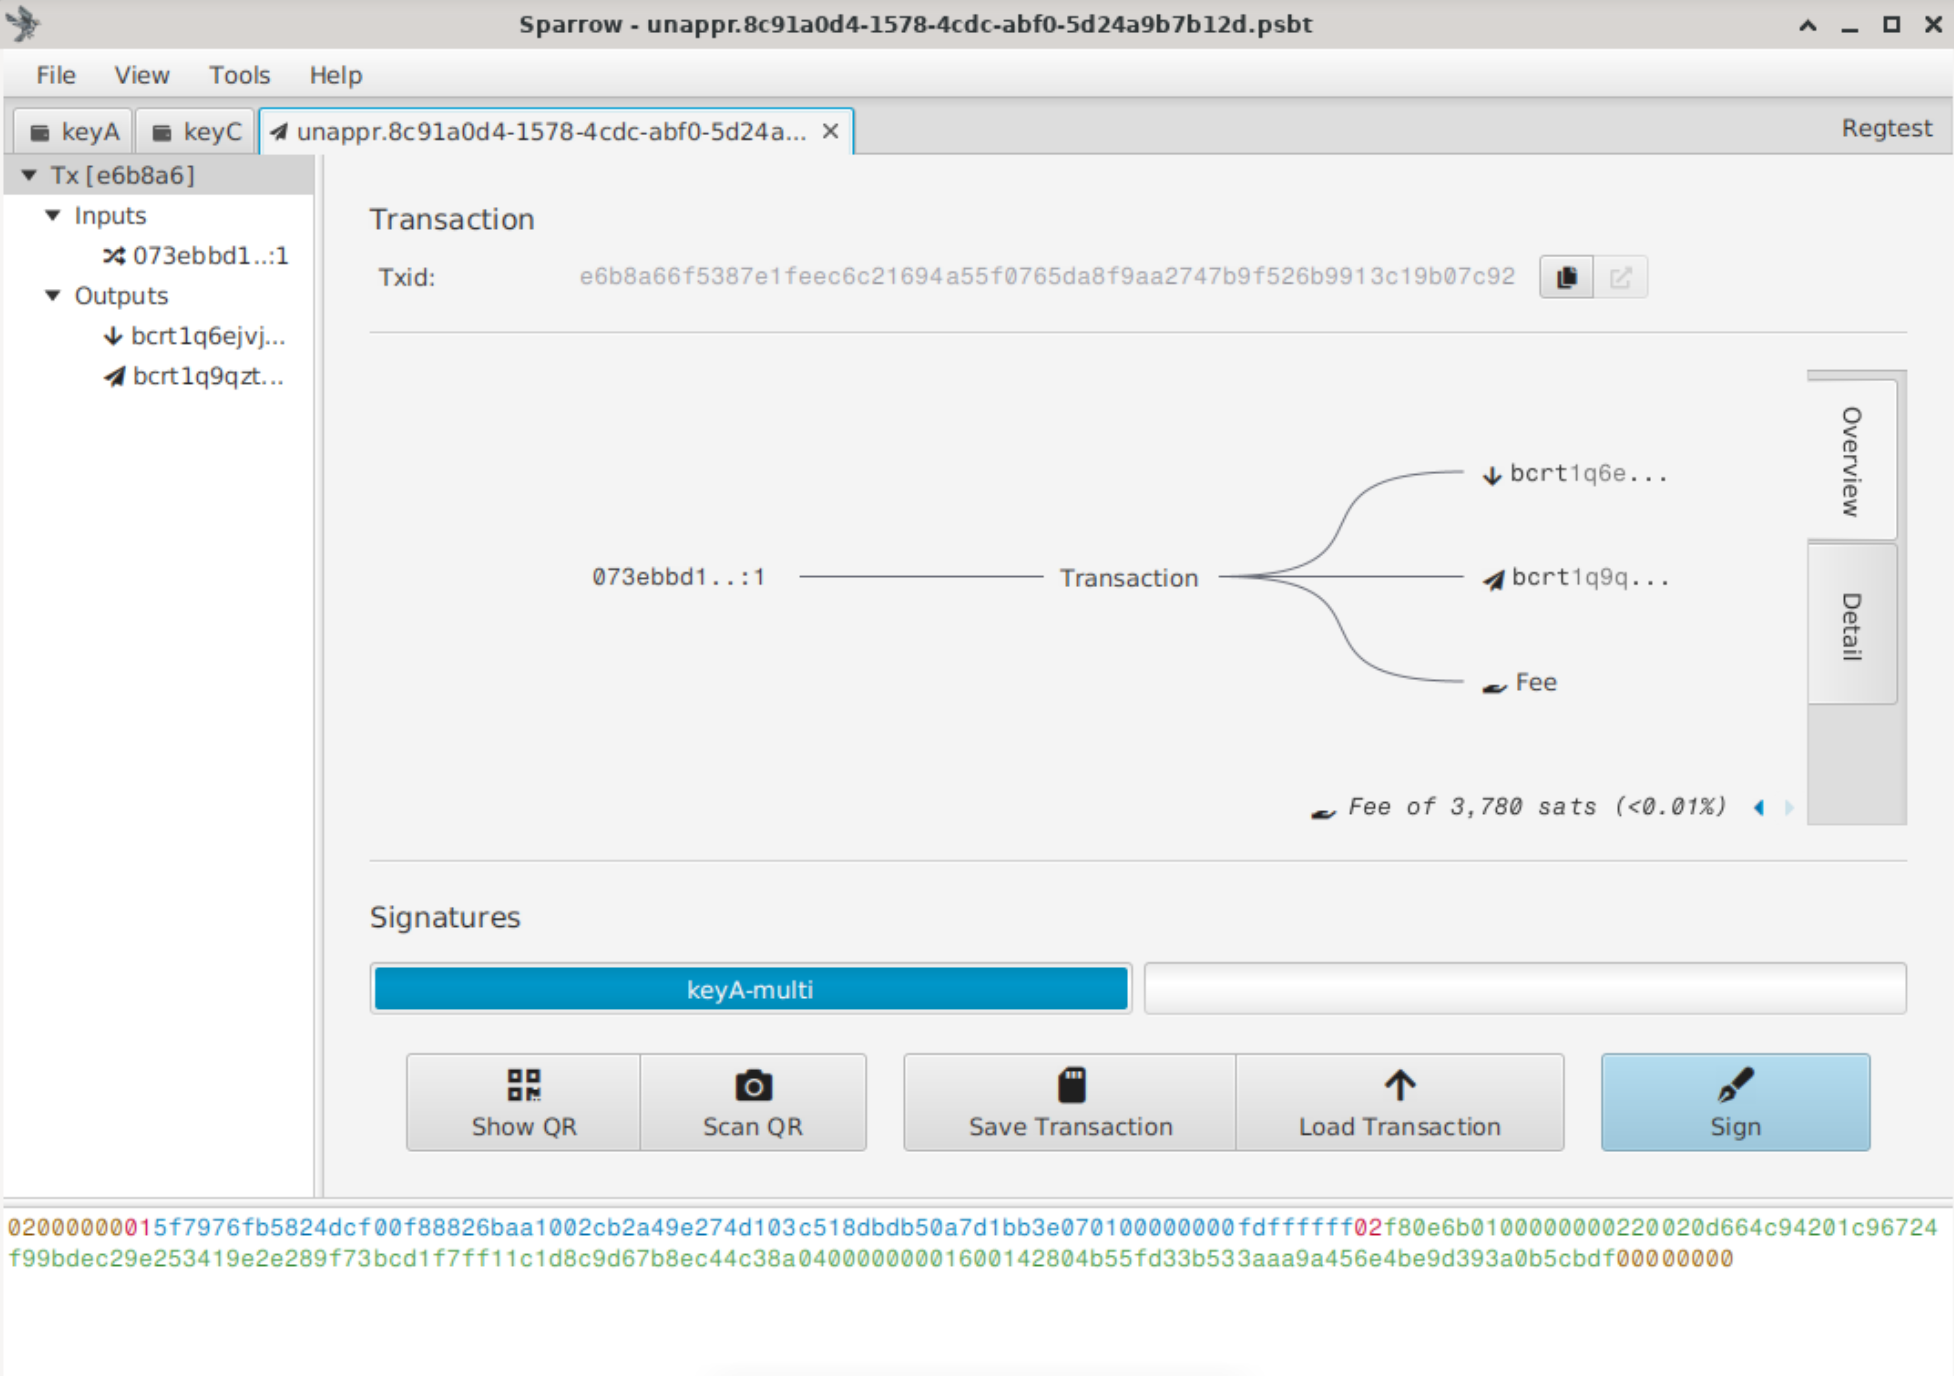
\includegraphics[width=0.8\textwidth]{Doku/Abbildungen/sparrow/sparrow_signing.png}
    \caption{Import mit vorsignierten Key~A Schlüssel. Quelle: Eigenes Bildschirm-Foto aus Sparrow.}
    \label{fig10:sparrow_keyA}
\end{figure}

Technisch wird dies umgesetzt, indem der Seed von Key~A für zwei verschiedene Pfade abgeleitet wird. Es handelt sich also um denselben physischen Schlüssel in zwei Deskriptor-Rollen.
\begin{itemize}
    \item \path{m/84'/1'/0'}: Als Single-Signatur für das Hot-Wallet nach \ac{BIP}84 und
    \item \path{m/48'/1'/0'/2'}: Als P2WSH-Cosigner für das Cold-Wallet nach \ac{BIP}48.
\end{itemize}

Der Ansatz stellt einen bewussten Kompromiss zwischen Operationalität und Isolation dar, wobei eine Schwächung des Sicherheitsniveaus des Cold-Wallets in Kauf genommen wird.
Wird das Hot-Wallet vollständig kompromittiert, so verfügt ein Angreifer bereits über einen der drei Cold-Schlüssel. Die effektive Hürde des Cold-Wallets reduziert sich damit aus Sicht des Angreifers von \enquote{zwei beliebige der drei Schlüssel} auf \enquote{einen weiteren der verbleibenden Schlüssel~B oder~C}.

Diese Schwächung ist im vorliegenden Bedrohungsmodell vertretbar, da sie ausschließlich die Cold-Schlüssel betrifft. Diese sind durch das Air-Gap genau gegen den Remote-Angriffsvektor abgesichert, der gegen das Hot-Wallet wirksam ist. Ein Angreifer müsste somit zusätzlich zur Hot-Kompromittierung den physischen Perimeter am Standort des Mandanten überwinden, der bis auf Angriffe über das Wechselmedium nicht Teil der Anforderungsbeschreibung des Mandanten ist.
Sollte ein Angreifer diese Hürden dennoch umgehen und einen Cold-Schlüssel extrahieren, wäre die Extraktion eines weiteren Schlüssels keine wesentlich größere Hürde, da Key~B und Key~C auf architektonisch identischen Maschinen liegen.

Umgekehrt ist das Hot-Wallet durch die TPM-Härtung von Key~A gegen genau diesen physischen Angriffsvektor stärker geschützt: Bei Aus- und Wiedereinbau der Hardware in ein anderes System würde das geheime Schlüsselmaterial nicht preisgegeben, da sich der Boot- und Konfigurationszustand und damit die \ac{PCR}-Bindung ändert.
Dementsprechend ergänzen sich Hot- und Cold-Wallet gegenseitig im Schutz der Mittel. Der maximale Schaden einer einfacheren, über das Online-System vollzogenen Kompromittierung bleibt dadurch auf den im Hot-Wallet vorgehaltenen Anteil von circa 5\,\% der Mittel beschränkt \cite{nist_zero_trust}.

Dem Mandanten bleibt es offen, dies durch Hinzufügen einer weiteren Cold-Signer-Maschine zu verschärfen und das Multi-Signatur-Verfahren auf 3-aus-4 zu erhöhen. Zu beachten bleibt, dass sich dadurch die für jeden \texttt{cold\_to\_hot}-Swap benötigte Zeit erhöht und sich damit die kritische Phase, in der die Operationalität des Hot-Wallets gefährdet ist, verlängert. Bei einem erhöhten Aufkommen automatischer Hot-Wallet-\acp{TX} und entsprechend vieler Nachbefüllungs-\acp{PSBT} kann dies einen deutlichen Unterschied ausmachen.

Ein Herauslösen von Key~A aus dem Cold-Wallet-Schlüsselsatz wird nicht empfohlen, da dadurch die Authentizitätssignatur des Hot-Systems und die darauf gestützte Verifikation der \ac{PSBT} entfielen.

\subsubsection{Doppelter Velocity-Check} \label{sec:doppelter_velocity}
Der Zweck der zwei örtlich getrennten Durchsetzungspunkte aus \ref{sec:OPA_vel} und \ref{sec:keyA_vel} liegt in der Abwehr eines mehrstufigen Angriffs. 
Auch wenn ein Angreifer das Basis-System unterwandert und den \ac{OPA}-Grenzwert durch Fälschen von \texttt{\seqsplit{spent\_today}} oder Umgehung der \ac{OPA}-Abfrage deaktivieren kann, bleibt der Signierer als zweiter, unabhängiger Enforcer bestehen.
Dieser deckelt den tatsächlichen Schlüssel-Abfluss über ein selbstkontrolliertes rollierendes Fenster und begrenzt den maximalen Schaden auf das vom Mandanten am Signierer konfigurierte Velocity-Limit. Dieses wird direkt aus den \acp{UTXO} der \ac{PSBT} berechnet und stellt sich als schwerer angreifbar dar. Dies überträgt das Prinzip der \emph{Segregation of Duties} auf die Abflusskontrolle und vermeidet einen Single Point of Compromise auch für das Velocity-Limit.
Eine mögliche Kompromittierung des Redis-Service, welcher sich auch auf diesen Sicherheits-Aspekt bezieht, wird im Folgenden behandelt (siehe \ref{sec:redis_schwach}).
Eine prägnante Darstellung dieses Sachverhalts kann in Tabelle~\ref{tab:limits} gefunden werden.

\begin{table}[htbp]
\centering
\footnotesize
\begin{tabular}{@{}p{3.2cm} p{4.6cm} l p{3.5cm}@{}}
\toprule
\textbf{Grenzwert} & \textbf{Zweck} & \textbf{Durchsetzungsort} & \textbf{Konfiguration} \\
\midrule
Betrag je \ac{TX} & begrenzt den Schaden einer einzelnen unautorisierten Zahlung & \ac{OPA} (Basis-System) & \path{data/data.json} \\
Gebühr je \ac{TX} & verhindert Mittelabfluss über überhöhte Gebühren & \ac{OPA} (Basis-System) & \path{data/data.json} \\
Tages-Abfluss & deckelt den kumulierten Abfluss regulärer Zahlungen & \ac{OPA} (Basis-System) & \texttt{max\_daily\_sats} \\
Velocity-Cap & unabhängiger Backstop, überlebt eine Kompromittierung des Basis-Systems & Signierer (Key~A \ac{VM}) & \texttt{VELOCITY\_CAP\_SATS}, \path{\
VELOCITY\_WINDOW\_SEC} \\
Hot-Balance-Zielbereich & steuert die Aufteilung der Mittel zwischen Hot- und Cold-Wallet & \ac{OPA} \texttt{hot.limits} & \path{data/data.json} \\
\ac{HMAC}-Zeitfenster & begrenzt die Wiederverwendbarkeit abgefangener Signieraufträge & Signierer (Key~A \ac{VM}) & Signer-Konfiguration \\
\bottomrule
\end{tabular}
\caption{Grenzwerte des Systems, ihr Zweck und ihre Durchsetzungsorte. Die
konkreten Werte sind Labor-Defaults und vom Mandanten an sein Mittelvolumen
anzupassen.}
\label{tab:limits}
\end{table}

Bei der Anpassung sind die Relationen der Grenzwerte zueinander zu erhalten.
Die Einzeltransaktions-Grenze liegt unterhalb des Daily-Caps, der Daily-Cap unterhalb des Velocity-Caps, sodass im Normalbetrieb stets die \ac{OPA}-Grenzen des Basis-Systems binden und der Signer-Cap ausschließlich als Backstop im Kompromittierungsfall greift. 
Der Velocity-Cap muss zudem genügend Puffer oberhalb des Daily-Caps besitzen, damit interne
Ausgleichs-Transaktionen nicht durch ihn blockiert werden. Die Grenzen des Balance-Zielbereichs sind so zu wählen, dass der Hot-Anteil dem gewünschten Risikoanteil (hier ca.\ 5\,\%) der Gesamtmittel entspricht.
Da Nachbefüllungen als Cold-Ausgaben nicht mitgezählt werden, bleibt der Rückfluss aus der Cold-Zone zudem auch bei ausgeschöpftem Cap stets möglich.

\subsubsection{Manipulierte Nachbefüllungs-\ac{PSBT}}
Der aus Angreifersicht attraktivste Pfad gegen die Cold-Bestände verläuft nicht über die Extraktion von Schlüsselmaterial, sondern über den regulären Nachbefüllungsprozess.
Ein vollständig kompromittiertes Basis-System kann eine Cold-\ac{PSBT} mit beliebiger Höhe und beliebiger Zieladresse erzeugen. Die internen \texttt{OPA\_cold}-Transaktionen durchlaufen weder die
Whitelist-Prüfung noch die Betragsgrenzen (siehe Tabelle~\ref{tab:tx_rails}) und Key~A signiert die \ac{PSBT} automatisch, da Multi-Signatur-Inputs vom Velocity-Cap ausgenommen sind (siehe \ref{sec:keyA_vel}). 
Die einzige und damit entscheidende Verteidigungslinie ist die manuelle Verifikation durch den Operator im Cold-System (siehe \ref{sec:sparrow_signierung}). Nur wenn die Zieladresse über das hinterlegte Watch-Only-Wallet eindeutig als zu Key~A gehörig aufgelöst wird und Betrag sowie Gebühren plausibel sind, darf signiert werden. 
Dieser bewusste \emph{Single Point of Human Failure} ist die Konsequenz des Air-Gaps, da eine automatische Prüfung im Cold-System dessen Isolation unterlaufen würde. 
Zur Verringerung des Restrisikos empfiehlt sich eine organisatorische Betragsobergrenze je Nachbefüllung, deren Überschreitung der Operator grundsätzlich als Kompromittierungsindiz wertet, sowie
perspektivisch ein Vier-Augen-Prinzip, bei dem Key~B und Key~C von verschiedenen Personen geführt werden.

\subsubsection{Wechselmedium}
Das \ac{USB}-Medium ist der einzige verbleibende Kanal in die Cold-Zone und wird von einem System beschrieben, dessen Kompromittierung das Bedrohungsmodell explizit unterstellt. Angriffe über manipulierte Dateisysteme oder \ac{USB}-Firmware (BadUSB) sind daher als Restrisiko zu betrachten. 
Die Cold-\acp{VM} begegnen dem durch deaktiviertes automatisches Mounten und ein minimales, deklarativ definiertes Softwareprofil. Verarbeitet werden ausschließlich \ac{PSBT}- und Deskriptor-Dateien, deren Inhalt in Sparrow vollständig angezeigt wird.
Zu beachten bleibt die bewusst aktivierte Doppelklick-Ausführung von Shell-Skripten im Dateimanager (siehe \ref{sec:cold_setup}): Sie gilt ausschließlich für die bei der Installation deklarativ auf dem Desktop abgelegten Skripte. 
Dateien vom Wechselmedium sind grundsätzlich nicht auszuführen, sodass das Medium ausschließlich als
Datenablage für \acp{PSBT} und Deskriptoren verwendet und vor jedem neuen Vorgang über das Format-Skript bereinigt wird. 
Eine Virtualisierung von \ac{QR}-Code-Übertragung war in der Laborumgebung nicht möglich (siehe
\ref{sec:alt_alg}). Im Produktivbetrieb stellt der Wechsel auf optische Übertragung die konsequente Schließung dieses Vektors dar.

\subsubsection{Redis Schwachpunkt} \label{sec:redis_schwach}
Sowohl die Nonce-Sperre als auch das Velocity-Fenster werden flüchtig in Redis gehalten und bewusst nicht persistiert. Der dauerhafte Schutz gegen das Wiedereinspielen vollständiger Signieraufträge ist die persistente \ac{PSBT}-\ac{ID}-Deduplizierung in der Datenbank. Die Nonce verengt lediglich das ohnehin kurze, über den Zeitstempel begrenzte Gültigkeitsfenster.

Dabei kann dieser Service durch einen Neustart direkt über Docker-Befehle oder über einen Denial-of-Service-Angriff, der einen Crash erzeugt, zurückgesetzt werden. Beide Angriffe wären durch eine Persistierung der Nonce und des täglichen Limits abschwächbar, jedoch wird diese Maßnahme als von nur schwachem Wert angesehen. Ein Angreifer, der bereits Zugriff auf Docker hat, kann auch das gesamte geheime Schlüsselmaterial auslesen oder persistente Datenbestände löschen. Ein Angreifer, der Denial-of-Service-Attacken als Peer des \ac{WG}-Tunnels ausführen kann, wird weiterhin durch das \ac{HMAC}-Geheimnis aufgehalten oder kann dieses ebenfalls umgehen und dem Signierer dann beliebige \acp{PSBT} über mehrere Tage unterbreiten, ohne dass ein Operator dies erkennen könnte.

Dementsprechend ist ein Angriff auf die Redis-Komponente nur bei einer fast vollständigen Kompromittierung möglich und kann vernachlässigt werden, da zu diesem Zeitpunkt einfachere Kompromittierungsziele bestehen. Gegen einen Angreifer auf dieser Ebene bilden ohnehin die \ac{TPM}-/\ac{PCR}-Bindung und die Prozess-Härtung die relevante Verteidigung, nicht die Flüchtigkeit von Redis. Bei Bedarf an einer über Neustarts hinweg auditierbaren Persistenz des Velocity-Fensters kann Redis mit AOF-/RDB-Persistenz betrieben werden. Hierauf wurde zugunsten einer minimalen Zustands- und Angriffsfläche verzichtet.

\subsubsection{Software-Lieferkette}
Ein air-gapped System ist gegen Remote-Angriffe isoliert, nicht jedoch gegen kompromittierte Software, die bereits bei der Installation eingebracht wird.
Die Architektur begegnet diesem Vektor durch den deklarativen NixOS-Ansatz, wobei sämtliche Pakete aus dem offiziellen, von den NixOS-Maintainern signierten Binary-Cache bezogen, und die vollständige Eingabemenge des Systems über einen gepinnten Flake (\path{flake.lock}) fixiert wird (siehe Tabelle~\ref{tab:nixos_hardening}). 
Dadurch ist reproduzierbar nachvollziehbar, welche Softwarestände auf den Schlüsselhalter-\acp{VM} laufen, und ein unbemerktes Nachladen veränderter Komponenten ist ausgeschlossen. 
Ein Restrisiko verbleibt in der Vertrauenskette zu den Upstream-Quellen selbst
(nixpkgs, Sparrow Wallet). Dieses kann durch die Verifikation der Upstream-Signaturen bei kontrollierten Updates weiter reduziert, jedoch prinzipiell nicht eliminiert werden. 
Updates der Cold-Systeme erfolgen ausschließlich als bewusste, manuelle Entscheidung des Operators.

\subsubsection{Rotation der Geheimnisse}
Die im System verwendeten Geheimnisse besitzen unterschiedliche Lebenszyklen und werden dementsprechend über getrennte Verfahren rotiert.

\emph{Laufzeit-Geheimnisse des Basis-Systems.} Die bei der Initialisierung zufällig erzeugten Zugangsdaten wie die \ac{NATS}-Passwörter der Dienst-Identitäten, das Operator-Token, das ntfy-Token, die PostgreSQL-Rollen-Passwörter sowie die \texttt{rpcauth}-Credentials von Bitcoin Core können über ein dediziertes Rotationsskript (\path{scripts/ops/setup/rotate_secrets.sh}) im laufenden Betrieb erneuert werden. Das Skript ersetzt die Werte nicht nur in der Laufzeitkonfiguration,
sondern setzt die \ac{DB}-Passwörter zusätzlich direkt in PostgreSQL (\texttt{ALTER ROLE}), sichert die vorherigen Stände mit Zeitstempel und erzeugt die betroffenen Container anschließend neu. Eine regelmäßige sowie eine anlassbezogene Rotation (etwa nach Personalwechsel oder Kompromittierungsverdacht) wird dem Mandanten empfohlen.

\emph{Systemübergreifende Geheimnisse.} Das \ac{HMAC}-Geheimnis liegt synchron auf Middleware und Signierer-\ac{VM} und wird bewusst nicht automatisch mitrotiert.
Beide Seiten müssen in einem Schritt getauscht werden, andernfalls weist die Signier-Schnittstelle sämtliche Anfragen ab. Die Rotation erfolgt daher kontrolliert über den etablierten Wechselmedium-Weg (\path{wgHMAC_export.sh} auf die Signierer-\ac{VM}, anschließend \path{wgHMAC_import.sh} auf dem Basis-System). Die WireGuard-Schlüsselpaare lassen sich analog über die Peer-Export- und Import-Skripte erneuern, wobei die vorherigen Schlüssel und Konfigurationen zeitgestempelt gesichert werden.

\emph{Wallet-Schlüsselmaterial.} Die Seeds selbst sind nicht im engeren Sinne rotierbar: Ein kompromittierter oder vorsorglich auszutauschender Schlüssel erfordert das Aufsetzen eines neuen Wallets und den Transfer der Bestände. Im Cold-Bereich genügen hierfür dank des 2-aus-3-Modells die
verbleibenden zwei Schlüssel, um sämtliche \acp{UTXO} auf ein neu erzeugtes Multi-Signatur-Wallet zu überführen.
Anschließend sind Deskriptoren und \acp{xpub} neu auszutauschen und auf dem Basis-System zu registrieren (analog zum Setup in \ref{sec:cold_setup}). Für Key~A ist zusätzlich die erneute Versiegelung im \ac{TPM} der Signierer-\ac{VM} vorzunehmen.

\subsubsection{Partner Authentifizierung} \label{sec:partner_auth}
Eine weitergehende Absicherung der externen Schnittstellen bestünde in einer expliziten Authentifizierung der Überweisungspartner, etwa über \ac{HMAC}-signierte Anfragen, Basic Authentication oder OAuth auf der \ac{HTTP}-Eingangsschnittstelle. Ein solches Verfahren ist jedoch stark partnerabhängig, da Schlüsselaustausch, Token-Format und Gültigkeitsdauer je Partner individuell ausgehandelt werden müssten. Daher wurde dieser Ansatz nicht als fester Bestandteil der Architektur umgesetzt. 
Die Authentizität eingehender Zahlungsanfragen wird stattdessen bereits teilweise durch das Whitelisting der Ziel-Wallet-Adressen abgedeckt: Da ausschließlich Transaktionen an registrierte, dem jeweiligen Partner zugeordnete Wallets signiert werden, bleibt die Wirkung einer gefälschten Anfrage begrenzt. Eine ergänzende partnerspezifische Authentifizierung bleibt dem Mandanten als Erweiterung im Approval-Gate offen.


\subsection{Fazit}

Die entwickelte Krypto-Architektur erfüllt die Kernanforderung des Mandanten:
Eingehende Zahlungsaufträge werden vollautomatisiert als Bitcoin-Transaktionen ausgeführt, ohne dass der überwiegende Teil der Mittel oder deren Schlüsselmaterial einem internet-exponierten System ausgesetzt ist. Erreicht wird dies durch die konsequente Trennung in drei Vertrauenszonen bestehend aus dem exponierten Basis-System, der gehärteten Signierer-\ac{VM} und der air-gapped Cold-Zone, zwischen denen ausschließlich \acp{PSBT}, niemals Schlüsselmaterial, ausgetauscht werden.

Die Sicherheit des Systems beruht dabei nicht auf einer einzelnen Maßnahme, sondern auf gestaffelten, voneinander unabhängigen Schichten: der \ac{OPA}-Autorisierung mit Whitelist- und Limit-Prüfung im Basis-System, der kryptographisch authentifizierten Übergabe an den Signierer (\ac{WG}, \ac{HMAC}, Deduplizierung), dem \ac{TPM}-versiegelten Schlüsselmaterial mit unabhängigem Velocity-Cap sowie dem 2-aus-3-Multi-Signatur-Modell mit verpflichtender manueller Verifikation im Cold-Prozess. 
Der maximale Schaden einer Kompromittierung des Online-Systems bleibt dadurch auf den im Hot-Wallet vorgehaltenen Anteil der Mittel begrenzt, zusätzlich gedeckelt durch die zweistufige Abflussbegrenzung.

Ebenso bewusst wurden die verbleibenden Grenzen des Modells benannt: 
Die Doppelnutzung von Key~A schwächt das Cold-Wallet kontrolliert zugunsten der Operationalität, die manuelle Verifikation durch den Operator bildet die letzte Verteidigungslinie des Nachbefüllungsprozesses, und das Wechselmedium bleibt der einzige, entsprechend restriktiv behandelte, Kanal in die Cold-Zone. Mehrere zunächst verfolgte Ansätze, darunter die Hash-basierte Freigabeschicht, der \ac{ZMQ}-basierte Eigenbau des \ac{UTXO}-Trackings und der netzwerkfähige Online-Koordinator, wurden nach Abwägung von Komplexität und Angriffsfläche bewusst verworfen. Die Reduktion auf das dargestellte Modell ist ein Ergebnis dieser Iterationen.

Für die produktive Übernahme verbleiben klar umrissene Schritte im Verantwortungsbereich des Mandanten: die Migration von Regtest auf das Mainnet (siehe \ref{sec:mainnet_migration}), der Betrieb der Zonen auf physisch getrennten Maschinen anstelle der virtualisierten Laborumgebung sowie optionale Verschärfungen wie ein 3-aus-4-Schema. Ergänzt werden kann ebenfalls die optische \ac{PSBT}-Übertragung per \ac{QR}-Code, ein NKey-/JWT-basiertes \ac{NATS}-Identitätsmodell und eine partnerspezifische Authentifizierung der Eingangsschnittstellen. 
Eine Härtung der \ac{TPM}-Bindung durch Secure Boot (unter NixOS über \texttt{lanzaboote}, Bindung an \ac{PCR}~7) und ein Unified Kernel Image (\ac{PCR}~11) samt signierter \ac{PCR}-Policy, die reguläre Updates ohne manuelles Neuversiegeln erlaubt, stellt eine weitere sinnvolle Ergänzung dar.
Zuletzt soll noch die Möglichkeit einer Retry-Queue für fehlgeschlagene Zahlungsaufträge erwähnt werden, deren Ausgestaltung jedoch stark von den Prozessen des Mandanten und seiner Partner abhängt. 
Die Architektur ist so ausgelegt, dass jede dieser Erweiterungen additiv möglich ist, ohne das Grundmodell zu verändern.

Eine abschließende Übersicht für den Krypto-Aspeckt dieser Ausarbeitung kann in Tabelle~\ref{tab:threat_matrix} gefunden werden.

\begin{table}[htbp]
\centering
\footnotesize
\begin{tabular}{@{}p{3.3cm} l p{4.0cm} p{3.4cm} l@{}}
\toprule
\textbf{Angriffsvektor} & \textbf{Zone} & \textbf{Gegenmaßnahme} & \textbf{Restrisiko} & \textbf{Verweis} \\
\midrule
Remote-Kompromittierung Basis-System & Hot & \ac{OPA}, Whitelist, Daily-Cap, 5\,\%-Aufteilung & Abfluss bis Velocity-Cap & \ref{sec:keyA_vel} \\
Manipulierte Nachbefüllungs-\ac{PSBT} & Hot$\to$Cold & Key-A-Vorsignatur, manuelle Sparrow-Verifikation & menschlicher Fehler & \ref{sec:sparrow_signierung} \\
Missbrauch des Operator-Pfads (Whitelist-/Limit-Bypass) & Hot & Besitz Operator-\ac{NATS}-Token, Struktur-/SHA-256-Prüfung, Daily-Cap, Velocity-Cap & Abfluss bis Velocity-Cap & \ref{sec:keyA_vel} \\
Replay von Signieraufträgen & Signierer & \ac{HMAC}, Nonce, \ac{ID}-Dedup & Redis-Reset & \ref{sec:redis_schwach} \\
Physischer Zugriff auf Key~A \ac{VM} & Signierer & \ac{TPM}/\ac{PCR}-Bindung, LUKS & Diebstahl des Seed-Backups & \ref{sec:doppelter_velocity} \\
Manipuliertes Wechselmedium & Cold & kein Automount, nur \ac{PSBT}-Dateien, manuelle Prüfung & BadUSB-Firmware & \ref{sec:sicherheitsbetrachtung} \\
Kompromittierte Lieferkette & alle & Flake-Pinning, deklarativer Neuaufbau & Upstream-Vertrauen & \ref{sec:sicherheitsbetrachtung} \\
Metadaten-Leak (Adress-/\ac{UTXO}-Abfragen) & Hot & eigener Bitcoin-Core-Full-Node statt öffentlichem Electrum-Server; dynamische Deskriptor-Adressen & On-Chain öffentlich einsehbar & \ref{sec:electrum_serv} \\
Verfügbarkeit des Hot-Wallets (Mittelmangel/\ac{DoS}) & Hot & automatischer \texttt{cold\_to\_hot}-Nachbefüllprozess, Monitoring/ntfy & manuelle Cold-Freigabe verzögert Rückfluss & \ref{sec:opa} \\
Böswilliger oder genötigter Operator & Cold & 2-aus-3 erfordert zweite Signatur; Vier-Augen-Prinzip als Ausblick & im Ein-Operator-Betrieb nicht abgedeckt & \ref{sec:sparrow_signierung} \\
\bottomrule
\end{tabular}
\caption{Bedrohungs- und Maßnahmenübersicht des Krypto-Systems (Bedrohungsmodell siehe \ref{sec:gefahrenmodell})}
\label{tab:threat_matrix}
\end{table}